%%%%%%%%%%%%%%%%%%%%%%%%%%%%%%%%%%%%%%%%%
% Short Sectioned Assignment LaTeX Template Version 1.0 (5/5/12)
% This template has been downloaded from: http://www.LaTeXTemplates.com
% Original author:  Frits Wenneker (http://www.howtotex.com)
% License: CC BY-NC-SA 3.0 (http://creativecommons.org/licenses/by-nc-sa/3.0/)
%%%%%%%%%%%%%%%%%%%%%%%%%%%%%%%%%%%%%%%%%

% \documentclass[paper=a4, fontsize=11pt]{scrartcl} % A4 paper and 11pt font size
\documentclass[11pt, a4paper]{book}
\usepackage[T1]{fontenc} % Use 8-bit encoding that has 256 glyphs
\usepackage[utf8]{inputenc}
\usepackage{fourier} % Use the Adobe Utopia font for the document - comment this line to return to the LaTeX default
\usepackage{listings} % para insertar código con formato similar al editor
\usepackage[spanish, es-tabla]{babel} % Selecciona el español para palabras introducidas automáticamente, p.ej. "septiembre" en la fecha y especifica que se use la palabra Tabla en vez de Cuadro
\usepackage{url} % ,href} %para incluir URLs e hipervínculos dentro del texto (aunque hay que instalar href)
\usepackage{graphics,graphicx, float} %para incluir imágenes y colocarlas
\usepackage[gen]{eurosym} %para incluir el símbolo del euro
\usepackage{cite} %para incluir citas del archivo <nombre>.bib
\usepackage{enumerate}
\usepackage{hyperref}
\usepackage{graphicx}
\usepackage{tabularx}
\usepackage{booktabs}
\usepackage{caption}
\usepackage{subcaption}

\usepackage[table,xcdraw]{xcolor}
\hypersetup{
	colorlinks=true,	% false: boxed links; true: colored links
	linkcolor=black,	% color of internal links
	urlcolor=cyan		% color of external links
}
\renewcommand{\familydefault}{\sfdefault}
\usepackage{fancyhdr} % Custom headers and footers
\pagestyle{fancyplain} % Makes all pages in the document conform to the custom headers and footers
\fancyhead[L]{} % Empty left header
\fancyhead[C]{} % Empty center header
\fancyhead[R]{Jose Luis Gallego Peña} % My name
\fancyfoot[L]{} % Empty left footer
\fancyfoot[C]{} % Empty center footer
\fancyfoot[R]{\thepage} % Page numbering for right footer
%\renewcommand{\headrulewidth}{0pt} % Remove header underlines
\renewcommand{\footrulewidth}{0pt} % Remove footer underlines
\setlength{\headheight}{13.6pt} % Customize the height of the header

\usepackage{titlesec, blindtext, color}
\definecolor{gray75}{gray}{0.75}
\definecolor{LightGray}{gray}{0.9}
\newcommand{\hsp}{\hspace{20pt}}
\titleformat{\chapter}[hang]{\Huge\bfseries}{\thechapter\hsp\textcolor{gray75}{|}\hsp}{0pt}{\Huge\bfseries}
\setcounter{secnumdepth}{4}
\usepackage[Lenny]{fncychap}


\begin{document}

	% Plantilla portada UGR
	\begin{titlepage}
\newlength{\centeroffset}
\setlength{\centeroffset}{-0.5\oddsidemargin}
\addtolength{\centeroffset}{0.5\evensidemargin}
\thispagestyle{empty}

\noindent\hspace*{\centeroffset}\begin{minipage}{\textwidth}

\centering

\includegraphics[width=0.9\textwidth]{logos/logo_ugr.jpg}\\[1.4cm]

\textsc{ \Large TRABAJO FIN DE MÁSTER\\[0.2 cm]}
\textsc{ MÁSTER EN INGENIERÍA INFORMÁTICA}\\[1 cm]

{\Huge\bfseries TropesToGo \\}
\noindent\rule[-1ex]{\textwidth}{3pt}\\[3.5 ex]
{\large\bfseries Scraping de TvTropes }
\end{minipage}

\vspace{2.5cm}
\noindent\hspace*{\centeroffset}
\begin{minipage}{\textwidth}
\centering

\textbf{Autor}\\ {Jose Luis Gallego Peña}\\[2.5 ex]
\textbf{Director}\\ {Juan Julián Merelo Guervós}\\[2 cm]

\includegraphics[width=0.3\textwidth]{logos/etsiit_logo.png}\\[0.1 cm]
\textsc{Escuela Técnica Superior de Ingenierías Informática y de Telecomunicación}\\
\textsc{---}\\
Granada, junio de 2023
\end{minipage}
\end{titlepage}


	% Plantilla prefacio UGR
	\thispagestyle{empty}

\begin{center}
{\large\bfseries TropesToGo \\ \textit{Scraping} de TvTropes }\\
\end{center}
\begin{center}
Jose Luis Gallego Peña\\
\end{center}

%\vspace{0.7cm}

\vspace{0.5cm}
\noindent\textbf{Palabras clave}: \textit{tropos}, \textit{TvTropes},
\textit{narrativa}, \textit{scraping}, \textit{crawling}, \textit{software
libre}, \textit{desarrollo ágil}, \textit{historias de usuario}, \textit{TDD},
\textit{DDD}, \textit{desarrollo incremental}, \textit{Go}, \textit{CLI},
\textit{logging}, \textit{CSV},
\textit{JSON}
\vspace{0.7cm}

\noindent\textbf{Resumen}\\
	
Los \textit{tropos} son unos recursos o patrones reconocibles que tienen un gran
interés en la generación de narrativas para que sus autores puedan transmitir al
público sus ideas de la manera más efectiva posible. Estos recursos son clave en
la popularidad que puede llegar a tener una obra, y están presentes en numerosos
medios audiovisuales como el cine, la televisión o los videojuegos. La
importancia de los \textit{tropos} suscita un gran interés que se ve reflejado
en la aparición de numerosos estudios, los cuales se revisan en este trabajo.
Estos estudios necesitan de un conjunto de datos amplio y completo que relacione
obras y \textit{tropos} para su análisis con técnicas estadísticas o
computacionales que permitan analizar el estado actual de la narrativa.

La web TvTropes es la mayor fuente de información sobre estos recursos. Contiene
una gran cantidad de datos semiestructurados que únicamente están pensados para
ser legibles por humanos y no están organizados ni preparados para su
procesamiento en un ordenador. En este trabajo se ofrece una solución a
investigadores y programadores para que puedan extraer estos datos según las
necesidades que tengan y puedan integrarlos en procesos de ciencia de datos que
propicien estos análisis.

A lo largo del trabajo se presenta un análisis de la web de TvTropes y se diseña
y desarrolla una herramienta de \textit{scraping} y \textit{crawling} en el
lenguaje Go que extrae información relevante de metadatos y \textit{tropos}
asociados de TvTropes. El objetivo de la solución es que sea capaz de entender,
extraer, limpiar y preparar los datos de cualquier página de \textit{tropos} de
TvTropes, genere ficheros de datos adecuados en formatos como CSV y JSON y
entienda la frecuencia con la que cambian los contenidos de TvTropes.

Para alcanzar los objetivos, se describe y lleva a cabo un proceso de desarrollo
ágil incremental guiado por historias de usuario, \textit{Test Driven
Development} y modelado con DDD que culmina en una herramienta de línea de
comandos libre llamada TropesToGo. Con esta herramienta, investigadores y
programadores pueden obtener conjuntos de datos de distinto formato y con la
información que necesitan. TropesToGo constituye una solución novedosa, ya que
hay muy pocos conjuntos de datos disponibles que asocien \textit{tropos} a obras
o herramientas que permitan extraer esta información de TvTropes.

\cleardoublepage

\begin{otherlanguage}{english}

\begin{center}
    {\large\bfseries TropesToGo \\ \textit{Scraping} from TvTropes}\\
\end{center}
\begin{center}
    Student's name\\
\end{center}
\vspace{0.5cm}
\noindent\textbf{Keywords}: \textit{tropes}, \textit{TvTropes},
\textit{narratives}, \textit{scraping}, \textit{crawling}, \textit{open source},
\textit{agile}, \textit{user stories}, \textit{TDD}, \textit{DDD},
\textit{incremental development}, \textit{Go}, \textit{CLI}, \textit{logging},
\textit{CSV},
\textit{JSON}
\vspace{0.7cm}

\noindent\textbf{Abstract}\\

Tropes are recognizable resources o patterns which are of great interest in the
generation of narratives so that authors can convey their ideas to the public in
an effective way. This resources are key in the popularity a work can reach, and
they are present in many media such as cinema, television or videogames. The
importance of tropes raises a great deal of interest in them that is reflected
in the emergence of numerous articles and studies, which are reviewed in this
paper. These studies require a large and complete dataset that links works to
its tropes so that computational or statisical analysis can allow new studies of
the current state of the narrative.

TvTropes is a website which holds the largest source of information on tropes.
It contains a great amount of unstructured data that is only intended to be
readable by humans, and is not organized or prepared to be processed by a
computer. In this paper a solution focused on programmers and researches is
proposed so that they can extract this data according to their needs and
integrate it into data science pipelines that will enable these studies.

Throughout this paper we present an analysis of the TvTropes website and design
and develop a scraping and crawling tool in the Go language that extracts
relevant information from TvTropes work metadata and its associated tropes. The
goal of the solution is to be able to understand, extract, clean and prepare
data from any TvTropes tropes page. It will be able to generate proper datasets,
in formats such as CSV or JSON, and understand the frequency with which TvTropes
contents changes.

To achieve the defined objectives, an incremental agile development process
guided by user stories, Test Driven Development and DDD modeling is described
and carried out. This culminates in a free and open source command line tool
called TropesToGo. With this tool, both programmers and researches can obtain
datasets in different formats with the exact data they need. TropesToGo is a
novel solution as there aren't many available datasets that link tropes to
works, or other tools that can extract this kind of information from TvTropes.

\end{otherlanguage}

\cleardoublepage

\thispagestyle{empty}

\noindent\rule[-1ex]{\textwidth}{2pt}\\[4.5ex]

D. \textbf{Juan Julián Merelo Guervós}, Profesor del departamento de Arquitectura y Tecnología de Computadores 

\vspace{0.5cm}

\textbf{Informo:}

\vspace{0.5cm}

Que el presente trabajo, titulado \textit{\textbf{Scraping de TvTropes}}, ha sido realizado bajo mi supervisión por \textbf{Jose Luis Gallego Peña}, y autorizo la defensa de dicho trabajo ante el tribunal que corresponda.

\vspace{0.5cm}

Y para que conste, expiden y firman el presente informe en Granada a junio de 2023.

\vspace{1cm}

\textbf{El director: }

\vspace{5cm}

\noindent \textbf{(Juan Julián Merelo Guervós)}

\chapter*{Agradecimientos}






	% Índice de contenidos
	\newpage
	\tableofcontents

	% Índice de imágenes y tablas
	\newpage
	\listoffigures

	% Si hay suficientes se incluirá dicho índice
	\listoftables 
	\newpage

	% Introducción 
	\chapter{Introducción}
En la creación y presentación de historias existen patrones reconocibles o
convenciones que llamaremos \textit{tropos}, o recursos reiterativos, que tienen
un gran interés como recursos de gran importancia para que los autores puedan
transmitir al público sus ideas. Cada medio tiene su propio lenguaje y forma de
expresarse, sin embargo, en todos ellos subyace la narrativa, que contiene estos
recursos reiterativos \cite{garcia2021simpsons}, por lo que se puede decir que
una obra de cualquier medio se define mejor como un conjunto de \textit{tropos}
\cite{garcia2020tropes}. El análisis de esta información mediante métodos de
ciencia de datos tiene gran interés en la construcción de modelos que ayuden a
los creadores de historias a entender mejor las relaciones que existen entre
estos \textit{tropos} y así crear historias mejores, que se adapten mejor a las
tendencias actuales y sean más interesantes y económicamente rentables. De esto
se deduce que es imprescindible tener un buen conjunto de estos datos para poder
construir modelos los más correctos, completos y actualizados posible.

Toda situación, arquetipo, convención o patrón que sea reconocible por la
audiencia y que se repita a lo largo de una historia se conoce en inglés como
\textit{trope}. Es importante destacar que este término no existe en español
\cite{tesisruben}, por lo que cuando se haga referencia a este concepto a lo
largo del documento se hará en cursiva, al ser una palabra informal, pero se
utilizarán también cualquiera de los otros términos que se han mencionado.

El concepto de \textit{tropo} está estrechamente relacionado con el concepto de
motivo, cuya definición es (Real Academia Española, 2023, definición 3): 

\begin{verbatim}
    ``En arte, rasgo característico que se repite 
    en una obra o en un conjunto de ellas''.
\end{verbatim}


Este rasgo que se repite puede ser una situación, un tipo de personaje, una
estructura narrativa o cualquier patrón que se utilice en la creación,
presentación o publicación de una historia, de forma que no la interrumpa (en
cuyo caso, sería un cliché) sino que ayude a entenderla y construirla mejor. Los
\textit{tropos} tienen interés como una parte imprescindible del puzle que es
producir una obra de cualquier medio, ya sea una serie, película, videojuego o
libro. 

Estos patrones se pueden analizar para obtener una serie de pautas que puedan
servir para crear nuevas obras más efectivas, por ejemplo analizando cómo
evoluciona el uso de \textit{tropos} a lo largo del tiempo y cuáles son los más
adecuados para representar un tipo de género o historia concreta. En resumen,
los \textit{tropos} son clave en la popularidad que puede llegar a tener una
obra y eso hace que surja en internet una comunidad dedicada a analizarlos,
entenderlos y almacenarlos llamada
TvTropes\footnote{\url{https://tvtropes.org/}}. 

TvTropes es un wiki abierto con contenido no estático cuyo principal cometido es
describir y almacenar ejemplos de \textit{tropos} en cualquier tipo de medio
audiovisual, cada uno de ellos con una descripción y ejemplos reales de dónde y
cómo se aplican. Sin embargo, la información de TvTropes va más allá de los
\textit{tropos}, con contenidos relativos a cualquier obra audiovisual agrupados
en sub-páginas como curiosidades, opiniones, información sobre actores o
personajes, vídeos, o cualquier otro tipo de apartado que la comunidad considere
interesante. Al ser un wiki que además usa su propio motor, a diferencia de
otros como MediaWiki que es libre y ampliamente usado y conocido, y que sus
contenidos están escritos y editados por los propios usuarios que lo visitan,
las páginas pueden variar tanto en forma como en contenido. TvTropes indica para
cada entrada de una obra audiovisual, entre otros, todos los \textit{tropos} que
la comunidad del sitio web ha identificado, explicando el por qué y añadiendo
ejemplos, siendo esta la principal fuente de información que proporciona la web.
Esta información está en constante crecimiento.

Sin embargo, tal y como se define en la propia web, el objetivo de TvTropes es
ser un wiki sobre \textit{tropos} que se utilizan para contar historias y
mostrarlos de un modo accesible y divertido de leer, destinado al usuario final.
Esta información no está estructurada y, por tanto, no existe una manera de
acceder a ella (mediante una API, por ejemplo) para su uso en ciencia de datos o
inteligencia artificial. Además de esto, TvTropes es una web centrada en los
\textit{tropos} y nada más que los \textit{tropos}, por lo que no manejan
información secundaria sobre los contenidos audiovisuales que tienen, los cuales
pueden ser también interesantes de analizar.

En estos análisis interesados en el estudio de \textit{tropos} en narrativas
entran trabajos de investigación como \cite{garcia2020tropes}, que describe
estadísticamente cómo se relacionan estos conceptos entre sí y cómo evolucionan
en el tiempo. Estos recursos reiterativos también se pueden combinar entre sí,
como en \cite{garcia2021simpsons}, que identifica qué combinaciones de
\textit{tropos} de películas son más usuales y cuáles pueden obtener buenas
reseñas y popularidad; y en \cite{any2vec}, que propone un modelo que analiza
conjuntos de tropos para su análisis mediante técnicas del procesamiento de
lenguaje natural. Este tipo de investigaciones parten de conjuntos de datos
distintos según las necesidades que tengan y, por tanto, actúan como principal
motivación de este proyecto, ya que, necesitan que estos conjuntos de datos
estén correctamente actualizados y preparados. De aquí surge la necesidad de una
buena herramienta que permita explorar cualquier página de TvTropes para extraer
exactamente los contenidos que se necesitan.

Explorar toda la información que provee TvTropes es todo un reto al ser una web
en constante cambio en la que la comunidad puede añadir nuevos \textit{tropos} o
películas, cambios en ellos o en sus relaciones, que requieren de estar siempre
al día con los contenidos. Entre el año 2016 y 2020 los \textit{tropos} que más
aparecen en películas fueron sustituidos por otros nuevos, el número de
películas aumentó en un $99.6\%$ y la media de \textit{tropos} en películas
aumentó un $279.38\%$\cite{garcia2020tropes}. Además, viendo la propia sección
de la web que indica todos los cambios que se hacen en
ella\footnote{\url{https://tvtropes.org/pmwiki/changes.php}}, se puede observar
como se realizan cambios, algunos de gran importancia etiquetados en la página
como \begin{otherlanguage}{english}``\textit{Large edit}''\end{otherlanguage},
diariamente. Todo esto muestra la rápida evolución de los contenidos de la web y
la importancia de estar al día con ellos. 

Por otro lado, existe información secundaria, como las fechas, que no está
estructurada y se encuentra dentro de un texto pensado solo para ser entendible
por un lector humano. Además, muchas de las páginas tienen distinta estructura
entre sí y esto dificulta el que un programa automático entienda la página que
está explorando. Estos son los principales problemas que se deben tener en
cuenta a la hora de construir una buena herramienta que sea capaz de extraer
esta información y representarla como un conjunto de datos analizable. La
resolución de estos problemas motiva este trabajo, que busca solucionarlos
mediante el desarrollo de un \textit{scraper}, un programa informático que sea
capaz de descargar, entender y organizar los datos de una web de forma autónoma
\cite{apress2018scraping}.

Varios de los trabajos de investigación mencionados usan una herramienta llamada
Tropescraper, un \textit{scraper} de TvTropes que no consigue extraer toda la
información que tiene la web actualmente, la cual ha cambiado bastante con el
tiempo, y que este proyecto usa como base de inspiración para mejorarla y
aumentar sus funcionalidades. En este trabajo se estudian los problemas que
tiene este \textit{scraper}, que se pueden resumir en que no explora
correctamente todas las páginas, requiere de un tiempo demasiado grande para
ejecutarse y extraer todos los contenidos, no está al día con los cambios en la
estructura de la wiki y que la información no se añade mediante incrementos por
lo que hay que relanzar de nuevo el scraper cuando se quieran actualizar los
datos. A esto se suman nuevas necesidades que surgen del proceso de estudio y
desarrollo a lo largo de este trabajo y que se pretenden resolver: el usuario
debe poder obtener solamente la información que necesita, sin necesidad de
explorar toda la web, y además poder obtener los datos en distintos formatos
estandarizados en ciencia de datos. En general, estudiar a los usuarios que se
beneficiarían de una herramienta de este tipo y comprender sus necesidades.

Por tanto, el propósito de este TFM es el de aportar una solución informática a
la extracción de datos de TvTropes teniendo en cuenta todas sus particularidades
y las necesidades de aquellos usuarios que usan la información de
\textit{tropos} para construir modelos y análisis; la necesidad de tener un
conjunto de datos bien preparado y limpio, la gran cantidad de información que
ofrece la web, el difícil acceso a esta debido a las distintas estructuras que
presenta TvTropes para presentarla por su condición de wiki y lo rápido que
evolucionan estos contenidos. Para lograr esto se construirá un \textit{scraper}
que sea capaz de entender y explorar la estructura de las páginas y contenidos
actuales de TvTropes para extraer su información. Con esta herramienta se quiere
que un usuario pueda obtener datos actualizados, correctos y preparados para su
análisis con métodos de ciencia de datos. Se busca además ampliar su
funcionalidad para que el \textit{scraper} obtenga información de metadatos
adicional y el usuario pueda extraer \textit{tropos} de cualquier medio
audiovisual, elegir qué partes de la información quiere según varios criterios y
elegir el formato de datos más adecuado para representarla.

Este trabajo se divide en tres partes diferenciadas:
\begin{itemize}
    \item En los \textbf{capítulos del 1 al 3} se entiende el trabajo y su
    contexto, describiendo el problema que se desea resolver y los objetivos que
    se quieren alcanzar, para luego en el estado del arte entender mejor el
    dominio del problema analizando las alternativas que existen actualmente en
    materia de scrapers y herramientas que extraen la información de la web de
    TvTropes, así como la situación actual de la propia página y los retos que
    presenta a la hora de extraer su información.
    \item La segunda parte, conformada por los \textbf{capítulos 4 y 5}, se
    centrará en los aspectos necesarios para poner el proyecto a punto,
    planificando su desarrollo, explicando la metodología a seguir, las
    herramientas que se utilizarán y modelando el problema para poder proceder a
    la implementación del \textit{software}.
    \item Por último, en los \textbf{capítulos 6 y 7} se desarrollará todo el
    trabajo realizado y cómo se ha llegado a la solución final, valorando
    finalmente si se han alcanzado los objetivos propuestos y qué se deja como
    trabajo para el futuro.
\end{itemize}

Este proyecto es software libre, está liberado con la licencia
GPLv3\footnote{\url{http://www.gnu.org/licenses/gpl.html}} y se puede encontrar
en un repositorio público de
GitHub\footnote{\url{https://github.com/jlgallego99/TropesToGo}}.



	% Descripción del problema y hasta donde se llega
	\chapter{Descripción del problema}

En este capítulo se desarrollará el problema que se ha introducido en la sección
anterior y que se quiere resolver, formulando los objetivos que se quieren
alcanzar al final del proyecto.

\section{Problema a resolver}
La importancia de los \textit{tropos} y su estudio en multitud de ámbitos con
métodos de ciencia de datos, como el análisis de \textit{tropos} más usados en
películas y cuáles son los más populares a lo largo del tiempo
\cite{garcia2020tropes}, o el análisis mediante algoritmos de combinaciones de
\textit{tropos} que permiten conocer qué nichos narrativos no han sido
explorados aún y pueden reportar un buen beneficio y críticas positivas
\cite{garcia2021simpsons}, abren la necesidad de tenerlos todos bien recogidos y
preparados para poder realizar un buen estudio de ellos con las herramientas
actuales que existen en ciencia de datos o inteligencia artificial. 

Es necesario poder extraer estos contenidos reiterativos completos o bajo algún
tipo de criterio, si es que se desea analizar un subconjunto de ellos. Y a esto
se le suma también el interés que pueden tener los metadatos de una obra, siendo
un problema el tener extraída por ejemplo una película con sus \textit{tropos}
asociados, pero que no se tenga más información de esta como puede ser el año de
publicación, el género, los actores, etc. Podrían existir análisis que
requiriesen de todos estos metadatos, por lo que necesitarían que esta
información extraída sea identificable con la de otras bases de datos, como
puede ser IMDB\footnote{\url{https://www.imdb.com/}} para el ejemplo de una
película.

La estructura de las páginas de TvTropes y sus contenidos están en constante
cambio, varias páginas están estructuradas de distintas maneras, algunas usando
un esquema más antiguo, otras uno más nuevo; algunas teniendo los
\textit{tropos} organizados por carpetas alfabéticas, otras teniéndolos en una
lista; información de tropos anidada dentro de otros, y muchos otros métodos de
organización que requieren de un extenso análisis para poder adaptarse a todas
las formas que presenta la web para dar su información. Para solucionar estos
problemas el \textit{scraper} debe conocer de antemano todas las estructuras que
puede tomar una página de TvTropes y comprobar que la página que está explorando
se adapta a alguna de las existentes y, por tanto, su información es extraíble.
Además, extraer tanta cantidad de información presenta un reto adicional en
términos de eficiencia en el tiempo de ejecución debido a todo el tiempo que
puede tardar una herramienta en recoger tantos contenidos.

El problema principal que busca resolver este trabajo es el de desarrollar una
herramienta eficiente y eficaz mediante la cual cualquier persona interesada en
el estudio de los \textit{tropos} pueda obtener todos los datos de TvTropes
estructurados y preparados para su análisis, pudiendo elegir qué información
concreta quiere sin necesidad de extraerla toda y en qué formato de datos la
quiere representada. Esta herramienta debe tener en cuenta la naturaleza
cambiante tanto de los datos como de la fuente de información de donde los
extrae, y debe poder presentarlos en un formato legible tanto por humanos como
por programas, para poder hacer cualquier tipo de estudio sobre ellos. Estos
datos deberán ser completos, correctos y estar siempre actualizados para evitar
que cualquier tipo de análisis esté desfasado.

A continuación se describen los objetivos que busca alcanzar este proyecto tras
haber resuelto los problemas descritos. Estos objetivos se usarán en la última
sección de este trabajo como medida para comprobar si el proyecto ha finalizado
correctamente.

\section{Objetivos}
Una vez descrito el problema que se quiere resolver y los retos que presenta, se
desglosan los objetivos específicos que tiene este trabajo.

\begin{itemize}
    \item \textbf{OBJ01} Diseñar y desarrollar un \textit{scraper} que opere de
    forma autónoma y sea capaz de entender y extraer la información de cualquier
    página de \textit{tropos} de TvTropes independientemente de su estructura.
    \item \textbf{OBJ02} Diseñar y desarrollar una araña que sea capaz de
    explorar todas las URL de páginas de \textit{tropos} que existen en TvTropes
    para poder lanzar el \textit{scraper} en ellas.
    \item \textbf{OBJ03} Diseñar y desarrollar una aplicación de línea de
    comandos mediante la cual el usuario pueda interaccionar con el
    \textit{scraper} eligiendo qué contenidos quiere extraer.
    \item \textbf{OBJ04} El \textit{scraper} entenderá la frecuencia con la que
    cambian los datos de TvTropes y actualizará la información extraída.
    \item \textbf{OBJ05} El \textit{scraper} desarrollado debe ser rápido y
    eficiente, adaptándose a la gran cantidad de datos que tiene que extraer.
    \item \textbf{OBJ06} El \textit{scraper} extraerá información de metadatos
    no estructurada que permita poder diferenciar entre obras audiovisuales y
    relacionarlas con fuentes de datos externas.
    \item \textbf{OBJ07} Los datos extraídos por el \textit{scraper} se
    almacenarán en distintos formatos de representación de datos usados en el
    ámbito de la ciencia de datos.
\end{itemize}



	% Estado del arte
	% 	1. Crítica al estado del arte
	% 	2. Propuesta
	\chapter{Estado del arte}

En este capítulo se hará una introducción de varios de los conceptos básicos que
se repetirán a lo largo de todo el trabajo, definiendo el estado actual de ellos
en la literatura y los desarrollos actuales que existen de proyectos de carácter
similar. Con esto se tendrá un mejor entendimiento del dominio del problema que
se analizará en profundidad en el capítulo 5 y se justificarán las herramientas
que se utilizarán en la implementación del software descrita en el capítulo 6.

El capítulo está dividido en dos secciones principales. En la primera sección se
describirán aspectos relativos al dominio del problema como qué es un
\textit{scraper}, sus necesidades y características actuales, además de los
diferentes formatos de representación de datos más comunes que existen en
ciencia de datos. En la segunda sección se analizarán otros trabajos
relacionados que tienen también como objetivo extraer la información de
\textit{tropos} de TvTropes. 

\section{Dominio del problema}
\subsection{Scraping}
El \textit{web scraping}, o extracción de datos web, se define como la
construcción de agentes que sean capaz de descargar, entender y organizar los
datos de una web de manera autónoma \cite{apress2018scraping}. 

A veces se usan los términos \textit{scraping} y \textit{crawling} de forma
intercambiable para hacer referencia a la misma idea de un programa autónomo que
explora una web y extrae su información, sin embargo, existe una distinción
concreta entre ambos. Cuando se habla de \textit{scraping} el enfoque es en la
extracción de datos en una página concreta de la que se conoce su URL. Por otro
lado, el \textit{crawling} (reptar o trepar) hace referencia a la exploración e
indexación de una web buscando cualquier tipo de información y explorando todos
los links que contiene, es decir, para descubrir toda una web completa, y suele
ser utilizado por los motores de búsqueda como Google \cite{scrapingvscrawling}.
Por tanto, son términos estrechamente relacionados, pero con distintos
objetivos; al desarrollar un \textit{scraper} se obtiene un conjunto de datos,
pero se necesita de un \textit{crawler}, o araña, para poder conocer y explorar
todas las URL que se quieren extraer y no se conocen de antemano.

Esta disciplina tiene especial interés para la ciencia de datos; concretamente
influye en la primera etapa de extracción de información, la cual debe estar lo
más limpia y lista posible para facilitar su posterior análisis. En internet
existe una gran cantidad de información no estructurada que, si bien un usuario
desde su navegador puede ver de una forma visual y agradable, no tiene fácil
acceso como conjunto de datos para su almacenamiento, limpieza y análisis de
cualquier tipo. Muchas webs proporcionan una API, a veces pública y a veces
privada, mediante la cual se puede acceder a sus datos o funcionalidades, sin
embargo, esto no siempre es el caso y es ahí donde el \textit{scraping} entra
para resolver estos problemas \cite{apress2018scraping}.

\cite{scraperworld, zhao2017web, olston2010web}

\subsection{Formatos de representación de datos}
Tabla comparativa
\section{Trabajos relacionados}
\subsection{Tropescraper}
La biblioteca
Tropescraper\footnote{\url{https://github.com/rhgarcia/tropescraper/}}
\cite{garcia2020startroper}

\subsection{DBTropes}
La web DBTropes\footnote{\url{http://skipforward.opendfki.de/wiki/DBTropes}}
\cite{kiesel2010dbtropes}

\subsection{Consejos sobre el scraping de TvTropes}
No existen demasiados proyectos \textit{software} en internet que se centren en
extraer la información de TvTropes además de los vistos anteriormente, lo cual
motiva este proyecto, ya que, puede aportar una solución que aún no existe a un
problema real. Artículos como \cite{gala2020analyzing}, que realiza un análisis
del sesgo de género que existe en los tropos narrativos, o
\cite{boyd2013spoiler}, que genera un modelo de aprendizaje automático para
detectar spoilers usando información de TvTropes, generan sus propios conjuntos
de datos ya sea con un \textit{scraper} o de otro modo sin dar mucha más
información de ello, puesto que se centran en el análisis. 

Sin embargo, el artículo de Sachita Nishal \cite{nishalscraping} presenta uno de
los pocos ejemplos reales que relatan el desarrollo de un \textit{scraper} de
TvTropes y las dificultades que presenta. En él se describe el proceso de
construcción del \textit{scraper} con el lenguaje Python a modo de ayuda para
cualquier interesado en extraer la información de esta web, y da una serie de
consejos que suponen un buen punto de partida para comenzar con el desarrollo
del \textit{software} de este trabajo. Además, el artículo sirve para tener en
cuenta muchas características de un desarrollo del mismo tipo, como los retos
que ofrece la estructura de TvTropes y cómo analizarla y explorarla de la mejor
forma posible, habiendo aprendido de los errores y dificultades de otra persona
al querer hacer lo mismo que pretende este trabajo.

Como se ha comentado al inicio de este trabajo, los contenidos de una página de
TvTropes no siempre están organizados igual. Generalmente, aunque todas las
páginas tienen un aspecto similar, presentan pequeños cambios significativos que
influyen enormemente en cómo estructuran la información y, por tanto, en cómo el
\textit{scraper} debe explorarlas \cite{nishalscraping}. El proceso seguido en
el artículo para extraer la información de la web y superar estos problemas es
el siguiente:
\begin{enumerate}
    \item \textbf{Definir qué se quiere extraer y por qué}
    
    En esta primera fase hay que pensar por qué queremos extraer información de
    una web y qué queremos concretamente, para así saber cómo organizar los
    datos mientras se van extrayendo. Esto hará que en el futuro la limpieza y
    procesado de estos datos sea más sencilla. Se destaca la importancia de
    diferenciar la extracción de la limpieza, siguiendo una estrategia de
    primero extraer toda la información que se pueda y decidir en fases más
    tardías con qué quedarse realmente.
    \item \textbf{Analizar la estructura general e identificar las excepciones}
    
    Una vez sabiendo qué se quiere extraer, el siguiente paso que siguió es el
    de mirar las distintas partes de la web y cómo están organizadas usando la
    herramienta de inspeccionar elemento de cualquier navegador web, que permite
    entender cómo están organizadas las etiquetas HTML en la web. Familiarizarse
    antes con cómo está organizada la web tanto por fuera como por dentro en las
    primeras fases del desarrollo permite estructurar mejor el código y saber
    desde el principio por dónde atacar.

    Identificar todas las excepciones mínimas en la plantilla de las páginas no
    es recomendable, ya que, como avisa el artículo, se puede volver una tarea
    inabarcable y sin fin. En su lugar se debe intentar no encontrar todas y
    cada una de las excepciones, sino construir el código de forma flexible para
    que sea capaz de tratar con aquellas excepciones que no se han identificado
    previamente.

    \item \textbf{Extraer la información}
    
    El propio proceso de \textit{scraping}, que requiere de una biblioteca que
    permita hacer peticiones HTTP para obtener el código HTML y que también
    pueda entender y transformar las etiquetas de la web en un árbol que sea
    fácilmente explorable por el programa para encontrar exactamente la
    información que se quiere. Además, conforme se vayan extrayendo los datos,
    se debe ir diciendo un formato adecuado en el que almacenar todos los datos
    que se quieren tener. Este formato permite que el programa tenga una idea de
    lo que tiene que buscar, ya que, aunque la estructura de cada página sea
    distinta, la información que se busca es siempre la misma.

    La estrategia que sigue el artículo es de primero extraer los datos y
    almacenarlos según sus etiquetas, almacenar el texto de cada una de las
    etiquetas independientemente de si servirán luego o no. Una vez se tiene
    esto, quedarse con lo verdaderamente importante limpiando los datos.

    \item \textbf{Elegir un formato para representar la información}
    
    El artículo finalmente hace hincapié en la importancia de representar los
    datos extraídos en un formato correcto para lo que se quiera, teniendo en
    cuenta factores como el poder usarlos en distintos lenguajes o la rapidez de
    lectura y escritura entre otros.
\end{enumerate}

Varias de las características que se identifican en \cite{nishalscraping} se
resumen en los siguientes puntos:
\begin{itemize}
    \item Cada página de una obra en TvTropes tiene una sección que contiene
    metadatos en forma de texto, y esto a veces se presenta en varios párrafos
    de resumen o dentro de una carpeta que el usuario tiene que hacer clic para
    abrir. 
    \item Los marcadores que indican que empieza una sección no se utilizan
    uniformemente en todas las páginas. Marcadores que indican, por ejemplo, la
    lista de actores de una película o la lista de tropos no siempre están
    presentes en todas las páginas.
    \item Los \textit{tropos} a veces están representados como una lista, otras
    veces están dentro de una carpeta e incluso existen páginas que listan los
    \textit{tropos} de varias películas distintas que están dentro de una
    franquicia.
    \item Es importante identificar los distintos marcadores de sección;
    concretamente el que precede a la lista de tropos suele ser del tipo
    \begin{otherlanguage}{english} ``This film contains examples of''
    \end{otherlanguage} cuando los tropos son para una sola película, mientras
    que cuando es para múltiples películas el texto es
    \begin{otherlanguage}{english} ``This series contains examples
    of''\end{otherlanguage}. En este último caso la palabra clave ``series''
    permite solucionar fácilmente el problema de páginas que hacen referencia a
    \textit{tropos} de múltiples obras.
    \item Toda la información útil de una página de TvTropes está contenida en
    el cuerpo principal y tiene unos mismos atributos \textit{id} y
    \textit{class}, por lo que este sería el punto de partida del
    \textit{scraper}, y a partir de aquí exploraría el resto de etiquetas según
    la página en la que se esté.
    \item Pueden aparecer menciones a \textit{tropos} dentro de la sección de
    resumen, fuera de la propia lista principal de la página, que pueden ser
    importantes también. En general, todos ellos suelen presentar el mismo
    atributo de clase ``twikilink'', por lo que el título del \textit{tropo} es
    fácilmente identificable.
\end{itemize}

Estas características se usarán como base en el capítulo 5 de este trabajo para
definir completamente las particularidades de la plantilla que presentan las
distintas páginas de TvTropes, analizar correctamente su estructura y saber cómo
proceder con la extracción de su información.

	
	\chapter{Planificación}
\label{chapter:4}

En este capítulo se especifican todas las cuestiones relativas a cómo se ha
abordado el desarrollo del proyecto con respecto a la planificación,
metodologías e infraestructura de control de calidad. 

Primero, se hará una introducción sobre la ingeniería del \textit{software} y la
metodología de desarrollo que se ha utilizado para guiar el completo desarrollo
del trabajo. A continuación, se definirán las buenas prácticas para garantizar
el control de calidad y que servirán para hacer un correcto seguimiento del
desarrollo, además del papel central que tiene GitHub en este. Por último, se
hará un estudio comparativo sobre las diferentes herramientas que existen para
asegurar estas buenas prácticas y cuáles se usarán finalmente en el proyecto.

\section{Metodología de desarrollo}
El proceso de desarrollo de un \textit{software} moderno implica tener en cuenta
ciertas verdades como el hecho de que tanto el \textit{software} como las
personas que lo consumen han crecido en número en los últimos años, y con ello
la demanda en adaptarlo y mejorarlo, lo que implica que cada vez se tienen
requerimientos tecnológicos más complejos. Esto implica que se debe hacer un
esfuerzo para entender el problema antes de desarrollar una aplicación
\textit{software}, siendo el diseño una actividad crucial, y además debe tener
una alta calidad y facilidad para recibir mantenimiento
\cite{pressman_software_2015}. Es aquí donde entra la ingeniería del
\textit{software}, la cual nos permite guiar este proyecto para superar los
problemas mencionados y alcanzar la excelencia técnica.

La ingeniería del \textit{software} es el establecimiento y uso de principios
fundamentales de la ingeniería con objeto de desarrollar \textit{software}
confiable y eficiente. Es un proceso que forma la base para el control de la
administración de proyectos \textit{software}, y establece el contexto en el que
se aplican métodos técnicos, se generan productos (modelos, documentación,
código, etc.), se establecen puntos de referencia, se asegura la calidad y se
aborda al cambio de manera apropiada \cite{pressman_software_2015}.

Debido a que las metodologías tradicionales son incapaces de abordar un
desarrollo moderno y no consiguen permanecer en el tiempo, siendo muy mecánicas,
con largos ciclos de desarrollo que requieren una larga planificación fija y
extensa documentación que no garantizan un producto de calidad, surgen una serie
de nuevos métodos conocidos como ``ágiles'' \cite{abrahamsson2017agile}. Estos
nuevos métodos pretenden resolver todos estos problemas, centrándose
principalmente en el usuario final y en la calidad, y que gozan de una gran
popularidad en la actualidad. En la actualidad la mayoría de proyectos que se
desarrollan siguen metodologías ágiles y tienen una mayor tasa de éxito,
consiguiendo mejores resultados en productividad, calidad del \textit{software}
y entregas al cliente más frecuentes con cambios frecuentes
\cite{agilestatistics}.

La creación de la metodología \textit{Extreme Programming} dio inicio a muchas
otras que se siguen utilizando actualmente, y aunque existen muchos marcos de
trabajo concretos para dotar de agilidad a un desarrollo, todos siguen los
mismos principios \cite{abrahamsson2017agile}. Estos principios fueron definidos
en el año 2001 en el manifiesto ágil \cite{agilemanifesto} y siguen vigentes a
día de hoy. En estos principios se definen como valores centrales el priorizar
las relaciones entre personas y sus capacidades sobre procesos predefinidos,
entregar constantemente nuevas versiones del \textit{software} testeado y
mantener una estrecha relación con el cliente con la que evolucione el contrato
y necesidades del proyecto en el ciclo de trabajo en lugar de tener algo fijo e
inalterable.

Cuando hablamos de agilidad estamos hablando de estar preparado a los cambios y
de ofrecer métodos para que los procesos de desarrollo sean más rápidos y
ligeros. En \cite{abrahamsson2017agile} se dan las características que definen
el desarrollo ágil: modularidad en los procesos de desarrollo, cortos ciclos
iterativos de una a seis semanas que permitan verificaciones y correcciones
rápidas, adaptación a riesgos emergentes, desarrollo incremental que permita
construir una aplicación funcional en pequeños pasos y minimice riesgos,
orientado a las personas y trabajo de forma colaborativa y comunicativa. 

Todo el proyecto se ha planteado siguiendo estos principios. Se ha elegido así,
puesto que es el tipo de desarrollo más utilizado en la actualidad y es más
flexible que el clásico desarrollo en cascada con requisitos fuertes que
requieren tener toda la información desde el principio y ceñirse estrictamente a
un plan prefijado, cosa que dificulta mucho el desarrollo e impide ponerse a
trabajar cuanto antes. Este enfoque ágil se adapta perfectamente a un proyecto
individual como este en el que se tienen unos requisitos débilmente definidos
que irán evolucionando conforme se vaya desentrañando la complejidad de TvTropes
y analizándolo para desarrollar el scraper, debido tanto a la necesidad de
desarrollar una herramienta que se adapte a las diversas necesidades de los
usuarios como al carácter que tiene este trabajo como proyecto de aprendizaje.

La flexibilidad que da el desarrollo ágil a la hora de detectar cambios permite
tener un enfoque más centrado en la implementación del \textit{software} y menos
en la documentación, pudiendo adaptarse a las nuevas necesidades que vayan
surgiendo, para tener un producto final tecnológicamente puntero, eficiente,
eficaz y de calidad que cumpla lo mejor posible los objetivos.

Por tanto, siguiendo los principios ágiles y sus ventajas anteriormente
definidas, se resumen las características del desarrollo de este proyecto como
las siguientes:

\begin{itemize}
    \item El desarrollo es iterativo e incremental, en el cual se definen una
    serie de hitos (o entregables) que conforman un Producto Mínimamente Viable
    (PMV). Este PMV conforma una parte de la funcionalidad total que se quiere
    tener al final para cumplir los objetivos especificados, siguiendo la idea
    del desarrollo ágil de entregas constantes de pequeños incrementos. Los
    tests se asegurarán de que este incremento sea completamente funcional,
    garantizando su calidad.
    \item El desarrollo está organizado por una serie de historias de usuario,
    que se utilizan en las metodologías ágiles para especificar los requisitos
    desde el punto de vista del usuario y con las que posteriormente se extraen
    las tareas de desarrollo, que especifican más concretamente los problemas de
    implementación que se quieren resolver y de qué manera. Las historias de
    usuario permiten organizar el desarrollo del proyecto, siempre teniendo en
    cuenta si satisfacen al usuario, que es para quien se desarrolla.
    \item Se acepta que surjan problemas o nuevos requisitos, que se
    documentarán adecuadamente y se incorporarán a la planificación en mitad del
    desarrollo para adaptarse a esos cambios lo antes posible y siempre cumplir
    las necesidades de los usuarios.
    \item Se busca siempre la calidad del \textit{software}, usando para ello
    las mejores prácticas del lenguaje tanto en código como en su documentación,
    usando diversas herramientas que faciliten la automatización de tareas como
    la compilación o el testeo. Se va a desarrollar una herramienta que en
    última instancia será utilizada por usuarios reales y estos deben obtener el
    mejor producto posible.
\end{itemize}

En las siguientes secciones se profundizará más sobre estas características del
desarrollo, introduciendo y describiendo los hitos e historias de usuario.
Además, con el propósito de cumplir correctamente todos los principios ágiles
que se han definido se emplean varias herramientas y buenas prácticas para el
seguimiento del desarrollo que se describen a continuación.

\section{Seguimiento del desarrollo}
En esta sección se introducirá todo el ecosistema de desarrollo que se empleará
en todo el trabajo para asegurar que se cumplan los objetivos. Primero se
describirá cómo será el proceso de desarrollo del código y su seguimiento a
través de la plataforma GitHub como herramienta central para guiar el proyecto
en su totalidad. A continuación, se describirán los distintos hitos que se
pretenden alcanzar consecutivamente. Finalmente, se estudiarán y justificarán
una serie de buenas prácticas y herramientas que se seguirán al escribir el
código y testearlo para asegurar la calidad y desarrollar correctamente el
\textit{software}.

\subsection{GitHub}
Al ser un proyecto de \textit{software} libre el uso de Git y GitHub como
\textit{software} de control de versiones es imprescindible. Esto permite tener
un seguimiento cercano de todos los avances que se hacen tanto en el código como
en la documentación, que están ambos alojados en el repositorio
público\footnote{\url{https://github.com/jlgallego99/TropesToGo}}. Además de
esto también facilita el poder recuperar versiones anteriores del
\textit{software} en caso de algún fallo o cambio sustancial, por lo que es
ideal en una metodología ágil en la cual existen constantemente cambios.

Sin embargo, lo más importante es que se guía todo el proceso de desarrollo
mediante el repositorio de GitHub, teniendo en un mismo lugar todo lo necesario
para hacer un correcto seguimiento del estado del trabajo que se tiene en
cualquier momento mediante las herramientas que proporciona GitHub. El
funcionamiento es el siguiente:
\begin{itemize}
    \item Para llevar el seguimiento de las historias de usuario y tareas
    asociadas a ellas de la metodología de desarrollo ágil se han creado una
    serie de \textit{issues} en el repositorio de GitHub que especifican el
    trabajo que hay que realizar. Estos \textit{issues} servirán para saber en
    todo momento en qué trabajar y siempre están orientadas a resolver una
    historia de usuario, es decir, satisfacer sus necesidades.\\
    Cada vez que, en mitad del desarrollo, se necesite desarrollar algo o
    solucionar un problema se documenta en un \textit{issue} que especifica qué
    se quiere conseguir y entonces se trabaja en cumplirlo.
    \item Los distintos hitos estarán documentados en la sección de
    \textit{milestones}, indicando a modo de resumen el objetivo que se pretende
    alcanzar al tener ese producto funcional. Este es el principal artefacto
    para conocer el estado del proyecto, ya que cada hito indica una fecha
    límite para completarlo y una serie de \textit{issues} necesarias para
    completarlo por completo. Conforme estas se van completando se puede ver
    cuánto trabajo queda por hacer.
    \item Cada \textit{commit} es un avance en el código o la documentación, y
    en el mensaje se hará una pequeña indicación que sirva para saber qué se ha
    hecho para avanzar en el \textit{issue} al que hace referencia. De esta
    manera podemos saber en todo momento las decisiones que se han tomado para
    resolver una determinada tarea, teniendo un historial con todos los cambios.
    \item Todo el código y documentación que esté en la rama principal del
    repositorio se entiende que está probado y, por tanto, es completamente
    funcional. \\
    El código se desarrolla en ramas separadas a la principal, que hacen
    referencia a cada hito que se quiere alcanzar. Cada vez que se complete una
    tarea de desarrollo se hará un \textit{pull request} a la rama principal, y
    si pasa los flujos de CI configurados (los cuales se explicarán en próximas
    secciones) entonces se dará la tarea por completada y se tendrá una nueva
    versión funcional en la rama principal. 
\end{itemize}

Como podemos ver, mediante GitHub se tiene en un mismo sitio todo lo necesario
para el desarrollo: código, documentación y seguimiento del desarrollo para
saber siempre el trabajo que se tiene que hacer y poder avanzar de una forma más
cómoda en alcanzar los objetivos y satisfacer al usuario. 

\subsection{Hitos}
Como se ha visto anteriormente, uno de los principios básicos del desarrollo
ágil es el de ir creando rápidamente pequeños incrementos funcionales del
producto para ir teniendo un \textit{feedback} continuo del cliente, abordar
cambios y problemas lo antes posible y así minimizar el riesgo. Cada uno de
estos incrementos lo representamos como un hito, o \textit{milestone}, que
representa cada uno de los estados en los que va a ir evolucionando el
\textit{software}, conformando un Producto Mínimamente Viable. Cada PMV se
construye encima de los anteriores, por lo que no se avanza en el desarrollo
hasta que un hito quede completo en su totalidad. 

Cada hito equivaldría a un sprint, que es un ciclo de desarrollo corto (y
debería durar entre 1 y 6 semanas \cite{abrahamsson2017agile}) en el que se
desarrolla todo lo necesario para resolver los \textit{issues} convenientes, que
se deducen de las historias de usuario definidas. Estos \textit{issues} siempre
expresan un problema, cuya resolución satisface una historia de usuario, y por
consiguiente, al cliente. Al final del sprint se consigue un incremento de valor
en el producto que se está construyendo, es decir, un PMV. 

Estos hitos se van adaptando al propio proceso de desarrollo y van cambiando a
lo largo del trabajo conforme surgen nuevas necesidades al entender mejor el
dominio del problema o al necesitar productos mínimos intermedios antes de poder
trabajar en el siguiente. Es posible que para conseguir llegar a cierto
incremento haya que realizar antes otro que no se haya tenido en cuenta desde el
principio; la flexibilidad del desarrollo ágil nos permite hacer estos cambios
de planificación sin tener que replantear todo desde cero.

Un \textit{milestone} se considerará como completado una vez se hayan resuelto
todos sus \textit{issues} asociados. Al terminarlo y subir sus cambios a la rama
principal (tras un \textit{pull request} que haya sido aprobado por los flujos
de CI y el tutor) se lanzará un nuevo \textit{release}, es decir, el propio
incremento del producto que tendrá un número de versión asociado siguiendo la
nomenclatura del versionado semántico\footnote{\url{https://semver.org/}}. En el
\autoref{chapter:6} se justificarán en orden todos los productos mínimos que
forman cada \textit{milestone}, por qué son necesarios y las decisiones tomadas
en cada uno para completarlo y poder avanzar en completar las historias de
usuario.

Los hitos que han ido surgiendo y completando a lo largo de todo el desarrollo
son los siguientes:

\subsubsection{M0. Configuración inicial - Objetivos, metodología e infraestructura de control de calidad}
En este primer hito se pretende abordar toda la planificación inicial y
preparación del proyecto para poder asegurar la calidad del mismo. Como producto
al final de este hito se definirán los hitos iniciales del proyecto y se tendrán
escritos los capítulos 1, 2, 3 y 4 de la documentación en los cuales se abordará
la descripción del problema a resolver, el estado del arte y toda la metodología
a seguir durante el proyecto. También se tendrá configurado el repositorio con
un comprobador ortográfico para la documentación, un gestor de tareas, los
sistemas de CI y los \textit{issues}, historias de usuario y \textit{milestones}
en el propio repositorio.

\subsubsection{M1. Modelización del problema}
Se obtendrá un producto mínimamente viable con el capítulo 5 de la
documentación, describiendo la metodología para modelar el problema durante el
desarrollo y analizando las partes más importantes de TvTropes, tanto el sitio
como la página. El modelo del problema permitirá definir tanto la organización
del código como las estructuras de datos e interfaces iniciales que permitan
resolver los dos próximos \textit{milestones} centrados en la extracción de
información de \textit{tropos} de las películas de TvTropes.

\subsubsection{M2. Scraper que entiende y testea una página de tropos de películas}
Con este hito se dará una primera versión funcional de un servicio
\textit{scraper} que sea capaz de encontrar el URL de una página sobre tropos de
películas en TvTropes, entienda su estructura y realice una serie de
comprobaciones sobre ella para confirmar que se pueda extraer información.

Al completar este hito se alcanza la primera
\href{https://github.com/jlgallego99/TropesToGo/releases/tag/v0.1.0}{versión
0.1.0} del \textit{software}, disponible en el repositorio de GitHub.

\subsubsection{M3. Scraper que extrae la información de una página de tropos de películas}
Se producirá un producto mínimamente viable que amplíe la funcionalidad del
scraper para poder extraer la información de la página principal de una
película, que ha sido previamente testeada y de la cual se entiende su
estructura. El scraper almacenará esta información en un fichero de datos
estándar.

Se lanza en el repositorio de GitHub la
\href{https://github.com/jlgallego99/TropesToGo/releases/tag/v0.1.0}{versión
0.2.0}.

\subsubsection{M4. Scraper que extrae tropos de las sub páginas de una película}
Con este hito se expande la extracción de \textit{tropos} anterior, con un
\textit{scraper} que pueda obtener todos los \textit{tropos} que tiene una
película en cualquiera de sus sub páginas. Estas sub páginas contienen
\textit{tropos} adicionales según distintas temáticas o, en algunos casos, son
parte de los \textit{tropos} principales de la película, que han sido divididos
en sub páginas debido a su gran volumen.

Se lanzan las versiones
\href{https://github.com/jlgallego99/TropesToGo/releases/tag/v0.3.0}{0.3.0} y
\href{https://github.com/jlgallego99/TropesToGo/releases/tag/v0.3.0}{0.4.0}, que
amplían el \textit{scraper} para la extracción sobre los distintos tipos de
subpáginas.

\subsubsection{M5. Araña que recorre el sitio}
Se tendrá desarrollado un servicio adicional: un \textit{crawler} que sea capaz
de encontrar todas las páginas de películas de TvTropes que sean relevantes,
para así poder extraer sus metadatos y \textit{tropos}.

En este PMV se lanza primero la
\href{https://github.com/jlgallego99/TropesToGo/releases/tag/v0.5.0}{versión
0.5.0} con la funcionalidad principal del \textit{crawler} y luego se mejora su
eficiencia y efectividad con las versiones
\href{https://github.com/jlgallego99/TropesToGo/releases/tag/v0.5.1}{0.5.1} y
\href{https://github.com/jlgallego99/TropesToGo/releases/tag/v0.5.1}{0.5.2} del
\textit{software}.

\subsubsection{M6. Actualizador de información}
El objetivo de este hito es poder actualizar aquella información ya extraída que
ha sido actualizada en TvTropes. Se tendrá como producto mínimamente viable una
araña que sea capaz de saber cuándo una página ha sido actualizada y las
encuentre todas ellas para volver a extraerlas y actualizar el conjunto de datos
sin tener que volver a lanzar el \textit{scraper} desde cero.

Se lanza una
\href{https://github.com/jlgallego99/TropesToGo/releases/tag/v0.6.0}{versión
0.6.0} con todo el código desarrollado para abordar la actualización de datos
extraídos.

\subsubsection{M7. Aplicación de extracción de tropos de múltiples medios audiovisuales}
Como producto de este hito se dará una primera aplicación ejecutable sencilla
que podrá utilizar el usuario final. Se tendrá una programa en el cual el
scraper y el crawler desarrollados previamente trabajarán en conjunto para
encontrar todas las páginas de obras con \textit{tropos}, pudiendo elegir entre
varios medios audiovisuales (videojuegos, libros, series, etc.) y extraerlos en
datasets de distinto formato (CSV o JSON).

\subsection{Desarrollo dirigido por pruebas}
El desarrollo dirigido por pruebas (TDD, de sus siglas en inglés \textit{Test
Driven Development}) es una de las principales y más importantes prácticas en el
marco de las metodologías ágiles para garantizar la calidad del
\textit{software}. Se trabaja bajo la idea de que cualquier código que no esté
testeado no es correcto, es propenso a fallos y, por tanto, todo el código debe
estar testeado para asegurar su buen funcionamiento y su calidad.

El objetivo del TDD es conseguir código limpio que funcione, y para ello es
necesario desarrollar primero los tests antes que el código de forma que al
estar trabajando en el código se tenga en cuenta qué tiene que cumplir. Esto
permite desarrollar de un modo predecible sabiendo siempre en qué momento se ha
terminado de desarrollar una tarea, ya que se ha realizado pensando en los tests
que tiene que pasar y estará testeada. 

El trabajar en un marco TDD da espacio a analizar bien el código, puesto que no
basta solo con desarrollar una función, sino que hay que estudiar bien su
funcionamiento para detectar todos los casos límite y probarlos. Además, tal y
como se busca en las metodologías ágiles, el objetivo del desarrollo dirigido
por pruebas es mejorar las vidas de los usuarios que usan el \textit{software}
\cite{beck2002driven}. En general, un código bien testeado se adapta a la
filosofía de cambio de las metodologías ágiles, ya que el reducir el riesgo
implica que el coste de abordar problemas o nuevas mejoras al desarrollo es
menor y puede suceder más frecuentemente.\\

La filosofía que se sigue a la hora de desarrollar tests es que estos son
automáticos y se desarrollan continuamente y siempre a la vez que el código. La
principal ventaja de esto es que ayuda a desarrollar bien el propio código al
tener en mente que los componentes que se desarrollan deben ser cohesivos y
tener un bajo acoplamiento para que escribir los propios tests sea una tarea
fácil.

Al desarrollar tests se sigue el \textit{mantra de TDD}, un orden definido por
Kent Beck \cite{beck2002driven} que consiste en: primero, hacer un test básico
que no funcione o no compile; segundo, arreglar el test para que funcione de la
forma más básica; y tercero, refactorizar y mejorar tanto el test como el código
sin cambiar la funcionalidad consiguiendo un código más simple y limpio. Todo
este proceso sigue la misma filosofía iterativa e incremental que la metodología
ágil que se usa en todo el desarrollo.\\

Por último, el desarrollo de los tests es también documentación, estando dentro
del propio lenguaje de programación. Los tests deberán ser legibles y
entendibles, centrándose en el comportamiento de las funcionalidades que evalúan
y, por tanto, permitirán expresar una correlación más directa con las historias
de usuario y la lógica de negocio.

\subsection{Integración continua}
La integración continua (CI, del inglés \textit{Continuous Integration}) es otra
práctica muy importante que se aplica en las metodologías ágiles y que está
estrechamente relacionada con la idea de cambio y de tener todo el código en un
repositorio central como el que se ha especificado. Las herramientas de
integración continua realizan comprobaciones automáticas sobre el código fuente
como paso previo al despliegue y crean algo ejecutable según las
especificaciones que se les dé, ya sea para crear un ejecutable del
\textit{software}, un test, un documento, un reporte, etc. En general se hace
referencia a cualquier proceso que automatice la construcción de una
aplicación.\\

En este proyecto se usan los sistemas de integración continua para automatizar
la ejecución de los tests y para comprobar ortográfica y gramaticalmente la
documentación al subir cambios a la rama principal, asegurando así la calidad
del \textit{software}, ya que todo el código que se tenga en producción estará
testeado. Esto además dota de agilidad al desarrollo, siguiendo con las mismas
ideas de metodologías ágiles, puesto que se tiene feedback en todo momento sobre
el estado de producción del código.

La razón de que se ejecuten estos sistemas para la rama principal es porque en
este proyecto se están desarrollando distintos productos mínimamente viables que
solamente estarán en la rama principal cuando se completen, y cuando no lo estén
se estarán desarrollando en alguna de las distintas ramas de desarrollo
correspondientes a cada hito, en la que no es necesario estar constantemente
ejecutando la integración continua. De esta manera aseguramos que todo el código
que esté en producción sea correcto porque ha pasado los tests
automáticamente.\\

Todos los sistemas de integración continua que se configuren se harán con GitHub
Actions para seguir con la idea de centralizar todo el desarrollo en el
repositorio de GitHub.

\section{Usuarios o partes interesadas}
Antes de definir las historias de usuario se analizan los usuarios o partes
interesadas en el proyecto (\textit{stakeholders}), para así poder enfocarlo en
resolver sus problemas. Este trabajo está orientado como un \textit{software}
que pueda integrarse en los procesos de ciencia de datos, por tanto, se ha
identificado un único usuario que representa el interesado en este ámbito:
\begin{itemize}
    \item \textbf{Investigador}: el investigador, o analista de datos,
    representa cualquier persona interesada en el estudio de los \textit{tropos}
    en narrativas para la generación de análisis y modelos de ciencia de datos y
    aprendizaje automático. Se asume que es una persona con cierto conocimiento
    informático y que sabe utilizar algún lenguaje de programación o herramienta
    de análisis de datos. Necesita tener la información estructurada y limpia de
    los tropos para construir modelos que le permitan hacer inferencias sobre
    las relaciones que tienen los tropos entre sí y llegar a conclusiones que
    sirvan para su investigación.
\end{itemize}

\section{\textit{User journeys}} 

Una vez definido el usuario para el que queremos desarrollar, es necesario
entenderlo para poder definir una serie de historias de usuario que expresen
correctamente sus necesidades. Para facilitar esto, desarrollamos una serie de
\textit{user journeys}, que describen, a modo de narración, todo lo que hace el
usuario desde que empieza a usar el \textit{software} hasta que termina, con el
objetivo de identificar distintas situaciones que nos permitan saber qué
desarrollar y de qué manera. En esta fase se tienen en cuenta aspectos como la
manera en la que accede al programa, para qué lo necesita, con qué frecuencia,
en qué contexto se encuentra, con qué dispositivo, los pasos para llegar a
solucionar su problema, etc. Esto nos dará una abstracción a alto nivel con la
que empatizar con los usuarios, entendiendo y representando cómo actuarían
finalmente al tratar con el \textit{software} que pretendemos construir. Este
enfoque permite desarrollar siempre con el usuario en mente, que es el objetivo
en el desarrollo ágil, y además ayuda a no solo contextualizar mejor las
historias de usuario, sino también a definirlas correctamente y poder generar
nuevas, al tener un punto del que partir.

Para desarrollar los distintos perfiles de usuario tenemos en cuenta los
artículos y líneas de investigación que se han ido mencionando a lo largo de
este documento. En estos se expresan las necesidades que tienen los
investigadores para tratar con \textit{tropos} y sus motivaciones, que a su vez
motivan a la creación de este proyecto y que sirven de ayuda para tener en mente
el tipo de personas a las que queremos ofrecerle una solución mediante
\textit{software}.

Para empezar con el proceso de generación de \textit{user journeys} definimos
los objetivos que se van a estudiar y que definen la razón de ser del
\textit{software} que se quiere desarrollar. Queremos estudiar los casos en los
que un investigador quiere obtener un conjunto de datos de películas con sus
\textit{tropos} y un conjunto de datos de toda la información de TvTropes, en
ambos casos para realizar algún tipo de investigación. A partir de esta premisa
buscamos varios caminos para que, mediante la experimentación, se lleguen a
cubrir varios mapas interesantes en los que el usuario alcance su objetivo.

\subsection{\textit{User journey} 1: Catedrático investigador en ciencia de
datos} 

Juan Benito García Martínez es un catedrático de la Universidad de Granada,
tiene 59 años y tanto la ciencia de datos como el aprendizaje automático entran
dentro de sus líneas de investigación.

\begin{itemize}
    \item Juan está trabajando en un artículo que estudia cómo los
    \textit{tropos} usados por películas influyen en el éxito que acabe teniendo
    tanto en taquilla como en crítica, estudiando también si existe algún cambio
    en los \textit{tropos} utilizados y el éxito cosechado a lo largo de los
    años.
    \item La fecha límite para entregar el artículo es dentro de una semana y
    aún necesita construir varios modelos de clasificación automática con tanto
    Python como R para cerrar el capítulo de análisis, así que necesita un
    fichero que contenga los datos que quiere. Está frustrado porque TvTropes no
    exporta su información y no tiene tiempo para trascribir tanta información a
    mano o construir una herramienta que lo haga por él.
    \item Decide buscar en internet para ver si alguien ya ha sacado esos datos.
    Encuentra varias recopilaciones de los datos de TvTropes que, sin embargo,
    datan del año 2016. Juan quiere que su artículo sea novedoso, ya que
    entiende que en los últimos años han salido muchas películas de renombre que
    han batido récords en taquilla. Tras una búsqueda más prolongada se
    encuentra con el repositorio de TropesToGo en GitHub, lee el \textit{README}
    del proyecto y se alegra al ver que le puede proporcionar justo lo que
    necesita: los datos de las películas y sus \textit{tropos} de TvTropes.
    Siguiendo las instrucciones del repositorio ve que es un programa que se
    puede instalar fácilmente con una sola orden, así que lo instala en su
    ordenador portátil.
    \item Siguiendo la documentación que hay en el repositorio encuentra
    rápidamente la opción que necesita. Juan ya ha usado aplicaciones de línea
    de comandos antes, por lo que, sin mucho problema ejecuta la orden exacta en
    el terminal especificando mediante varios \textit{flags} que quiere obtener
    un conjunto de datos en formato CSV para poder cargarlo con los dos
    lenguajes que va a utilizar y que quiere únicamente los \textit{tropos} de
    todas las películas que existan.
    \item Juan observa cómo en el terminal aparecen varios mensajes que le
    indican el estado del programa, que muestra cuántos \textit{tropos} lleva
    extraídos en cada momento. Juan está muy impaciente, pero de repente aparece
    un último mensaje que le indica que ya está listo su fichero, lo que le
    sorprende. Juan va a la ruta que ha especificado al ejecutar el comando y se
    encuentra con el fichero. Tras observarlo durante unos instantes está
    satisfecho, ya que entiende rápidamente cómo están codificados los datos y
    que contiene justo lo que necesita. Aún queda día, así que puede ponerse ya
    a trabajar. 
    \item Finalmente, ha podido entregar el artículo antes de tiempo gracias a
    lo rápido que ha conseguido el conjunto de datos y a que no ha necesitado
    realizar demasiadas tareas para limpiar los datos, puesto que ya estaban
    bastante utilizables. Contento y satisfecho, decide dejar instalado el
    programa en su ordenador por si necesitase otros datos de TvTropes para
    futuros análisis.
\end{itemize}

\subsection{\textit{User journey} 2: Estudiante de máster en ciencia de datos}

María Conde Alcaraz tiene 23 años y está terminando de estudiar el máster en
ciencia de datos en la Universidad de Granada.

\begin{itemize}
    \item María aprendió a utilizar TropesToGo al empezar a redactar su trabajo
    fin de máster, en el que tiene que construir un clasificador binario lo más
    preciso posible que permita identificar si un conjunto de \textit{tropos}
    pueden formar una serie de televisión que aguante en emisión varias
    temporadas.
    \item María se dio cuenta de que para su clasificador necesitaba más
    información de la que le provee el conjunto de datos que genera TropesToGo,
    principalmente el número de temporadas de una serie. Para solucionar esto,
    usó la información que ya posee, el título de la serie y el año en el que
    salió, para poder identificar la información adicional que necesita de otro
    lado. De esta manera, añade a su programa clasificador un módulo que se
    comunica con IMDB para sacar el número de temporadas que tiene cada una de
    las series que tiene en su conjunto de datos, añadiéndole un campo nuevo. Se
    siente aliviada, puesto que ha podido resolver fácilmente el problema
    gracias a la simplicidad y efectividad del conjunto de datos que tenía, que
    permitía relacionar las series fácilmente y no confundir las que tienen un
    mismo nombre.
    \item 6 meses después, queda un mes para la entrega del TFM y se da cuenta
    de que en ese tiempo TvTropes ha añadido muchísimos \textit{tropos} y
    series, que han tenido mucho tirón en ese periodo. María se siente. Sin
    embargo, vuelve a ejecutar TropesToGo con las mismas opciones que había
    utilizado anteriormente, y en muy poco tiempo el programa le informa de las
    series que se han actualizado en el conjunto de datos que ya tenía, por lo
    que, puede volver a ejecutar los modelos tal y como los tenía programados
    sin cambiar nada.
    \item María queda ahora muy satisfecha; podrá ir actualizando su conjunto de
    datos con el tiempo para que su clasificador automático entrene siempre con
    los últimos datos existentes.
\end{itemize}

\subsection{\textit{User journey} 3: Estudiante de un grado no relacionado con
la informática} 

Pablo Antonio Molina Ocaña es un estudiante del grado en estadística en la
Universidad de Granada. Es una persona joven, de 19 años, que únicamente usa un
ordenador muy básico para sus tareas de la universidad y es capaz de controlarlo
de forma básica en términos de usuario.

\begin{itemize}
    \item Pablo es un cinéfilo que pertenece a la comunidad de TvTropes, por lo
    que está muy familiarizado con lo que ofrece la página y tiene gran interés
    en ello. En clase le mandan un trabajo libre, y él decide que quiere hacerlo
    sobre los \textit{tropos} de sus películas favoritas y cómo se relacionan
    entre sí.
    \item Pablo es muy perezoso y no quiere escribir a mano toda la información
    que necesita de las películas que le gustan. Él está acostumbrado a tratar
    con el formato JSON y un \textit{software} que le permite sacar múltiples
    gráficas estadísticas basándose en el fichero que introduce. Buscando
    encuentra muy pocos conjuntos de datos de TvTropes, y la mayoría tienen más
    de lo que quiere y en otros formatos que desconoce, como CSV. Finalmente, se
    encuentra con TropesToGo y prueba a instalarlo en su ordenador portátil.
    \item Pablo no entiende muy bien cómo funciona el programa ni se ha parado a
    leer la documentación. Simplemente, lo ejecuta, y este le informa de lo que
    es el programa, lo que hace y le da varias opciones que él puede seguir.
    Introduce con su teclado que solo quiere obtener los \textit{tropos} de tres
    películas que le gustan. El programa le indica que debe introducir la URL de
    TvTropes de la película que quiere extraer, cosa que Pablo sí conoce, así
    que lo hace. Finalmente, el programa le ofrece varias opciones simples de
    cómo quiere obtener los datos, a lo que pablo selecciona la opción de JSON.
    \item Observa como rápidamente el programa le indica que ya está todo listo,
    y le informa de dónde puede encontrar el fichero JSON con los datos de la
    película que necesitaba. Pablo repite el proceso para las otras que necesita
    y, viendo lo sencillo que es, se emociona y decide extraer unas cuantas más
    de las que tenía pensadas en un primer lugar.
    \item Al final consigue los datos que necesitaba y puede terminar su trabajo
    sin demasiadas complicaciones, lo que deja a Pablo con una gran sensación de
    autorrealización.
\end{itemize}

\subsection{\textit{User journey} 4: Profesora de ingeniería informática} 

Paula Millán Sánchez es una profesora de 45 años en el máster en ingeniería
informática de la Universidad de Granada que imparte una asignatura sobre
tratamiento inteligente de datos.

\begin{itemize}
    \item Paula está preparando una práctica final para la evaluación de la
    asignatura que imparte. La práctica consiste en que los estudiantes analicen
    varias maneras de tratar con gran volumen de datos. Para esto, necesita
    proporcionarles un gran conjunto de datos en un formato que entiendan.
    \item Encuentra TropesToGo en su repositorio público de GitHub tras la
    recomendación de otro profesor, y decide ejecutar directamente el programa.
    La aplicación le da distintas opciones que le indican qué conjuntos de datos
    puede obtener y elige que quiere obtener un conjunto de datos con toda la
    información de TvTropes. Satisfecha, deja el ordenador ejecutándose y se va
    al gimnasio.
    \item Cuando vuelve, se da cuenta de que ha habido un apagón en su casa.
    Frustrada, enciende su ordenador de nuevo, muy agobiada sabiendo que
    seguramente haya perdido todo el progreso del programa.
    \item Siente incertidumbre porque no sabe si ha perdido todo el progreso que
    tenía. Vuelve a elegir las mismas opciones que antes y la aplicación le
    indica que ya tiene datos descargados en su ordenador y que seguirá
    descargando los que falten. Entusiasmada, Paula ve que la aplicación le va
    informando del progreso, que indica cuándo está extrayendo datos nuevos y
    cuándo está ignorando los que ya se tienen. El programa termina en 5
    minutos, informándola de que ya está todo hecho. Parece ser que antes del
    apagón estaba ya completado casi todo el proceso, así que solo ha requerido
    un poco más de tiempo. 
    \item Se siente alegre al no haber perdido el tiempo ejecutándolo todo desde
    el principio. Ahora Paula podrá mandarles el fichero con los datos a sus
    alumnos.
\end{itemize}

De estos \textit{user journeys} podemos sacar varias conclusiones, como por
ejemplo para qué pueden los usuarios necesitar los datos, que los investigadores
pueden utilizar distintos lenguajes de programación, que valoran muy
positivamente un conjunto de datos limpio y preparado para ahorrarles trabajo o
que quieren desarrollar análisis vanguardistas. También se hace referencia a
cómo interactúan con la aplicación final y las facilidades o dificultades que
pueden encontrar, como encontrar documentación que les permita saber cómo usar
la herramienta o que el propio programa les ayude a conseguir lo que necesitan
sin perder mucho el tiempo. Estas necesidades identificadas a lo largo de este
proceso se tendrán en cuenta a la hora de implementar el \textit{software}, para
cumplir con lo que los usuarios como los de este análisis esperan del producto
final, y se condensan a continuación en forma de historias de usuario, que serán
el principal artefacto que nos dirá cómo proceder con el desarrollo.

\section{Historias de usuario}
Sabiendo el problema que se quiere resolver y las partes interesadas se pueden
definir las historias de usuario que guiarán todo el desarrollo de principio a
fin, ayudando en la toma de decisiones para llegar a cumplir los objetivos.

\subsection{[HU01] Investigador - Obtener información sobre tropos}
Como investigador necesito poder obtener información sobre todos los tropos
existentes de cualquier tipo de medio audiovisual, en un formato estandarizado y
con una estructura definida para que sean de fácil acceso tanto a humanos como
programas para su análisis.

\subsection{[HU02] Investigador - Obtener un subconjunto de la información}
Como investigador necesito poder elegir qué parte de la información sobre tropos
quiero obtener, ya sea de un medio audiovisual concreto, todo un género, etc.

\subsection{[HU03] Investigador - Relacionar medios audiovisuales con fuentes externas}
Como investigador necesito obtener información de metadatos sobre cualquier
medio audiovisual, para lo cual necesito que los medios audiovisuales de los
cuales se han sacado sus tropos sean fácilmente identificables y se puedan
relacionar con su ficha en IMDB u otras fuentes de datos externas del mismo
tipo.

\subsection{[HU04] Investigador - Información actualizada}
Como investigador quiero que la información de tropos que obtenga esté lo más
actualizada posible, sepa cuándo se ha extraído y pueda obtenerla actualizada
cuando quiera para traer la nueva información que pueda existir, ya que TvTropes
es una página que cambia constantemente, tanto en estructura como en contenidos.

\subsection{[HU05] Investigador - Representación de los datos}
Como investigador quiero poder elegir el formato en el que se represente el
conjunto de datos de entre los más comunes en ciencia de datos.

\subsection{[HU06] Investigador - Inmediatez de los datos}
Como investigador quiero obtener lo más rápido posible y sin complicaciones el
conjunto de datos con lo que necesito para poder centrarme cuanto antes en
analizarlos para mi trabajo.

\subsection{[HU07] Investigador - Recuperación de datos}
Como investigador necesito poder publicar el conjunto de datos obtenido, acceder
a él y recuperarlo en cualquier momento, incluso de forma offline.

\subsection{[HU08] Investigador - Relación entre tropos}
Como investigador necesito conocer información adicional de los \textit{tropos}
que los definan mejor y me permitan relacionarlos entre ellos para poder crear
ontologías.

%\section{Temporización} Una vez vistos los hitos que se esperan alcanzar en el
%desarrollo, los cuales conformarían cada uno un sprint con una fecha de inicio
%y de fin, podemos representar la temporización de todo el desarrollo en un
%diagrama de Gantt.

%A lo largo de todo el desarrollo se ha ido manteniendo contacto con el tutor
%tanto en tutorías presenciales como mediante mensajes por Telegram y GitHub
%para transmitir y resolver todas las dudas que han ido surgiendo, tanto del
%código como del propio documento.

\section{Elección de herramientas para el desarrollo}
Al llevar un proyecto de ingeniería del software a la práctica, en el cual se
tiene como primer objetivo la calidad, se requieren herramientas para poder
llevar a cabo todas las buenas prácticas descritas a lo largo de este capítulo. 

Es por esto que por último se comentarán todas las herramientas que se van a
utilizar para desarrollar el propio software, comenzando por el propio lenguaje
de programación en el que se escribirá el código. También se justificarán
herramientas para tener un buen ecosistema de desarrollo en el repositorio de
GitHub y cumplir con las buenas prácticas que se han descrito en las secciones
anteriores. Se justifica la elección de cada una comparando entre varias
alternativas, teniendo en cuenta las características concretas de este proyecto
y siempre con la calidad como criterio más importante para elegir la más
adecuada.

\subsection{Lenguaje de programación}
La principal herramienta a considerar para construir un \textit{software} es el
lenguaje de programación, concretamente uno que se adapte a las necesidades de
este proyecto. Se puede desarrollar un \textit{scraper} en cualquier lenguaje de
programación, sin embargo, debido a la naturaleza de aplicación en red de este,
se busca un lenguaje de programación que sea bastante afín a trabajar con el
protocolo HTTP y sea para poder gestionar el gran volumen de datos que se
tratará y además sea concurrente para intentar mejorar el ritmo de las
peticiones del \textit{crawler}, como se comentó en el estado del arte.

Teniendo en cuenta esto, se elegirá Go\footnote{\url{https://go.dev/}} como el
lenguaje de programación para desarrollar el \textit{scraper} de este proyecto.
Go es un lenguaje de programación libre, concurrente, rápido, fácil de utilizar
y con una sintaxis muy legible y moderna, que facilita mucho el reestructurar y
reescribir el código. Además, una de las principales ventajas de Go con respecto
a otros lenguajes es que tiene una biblioteca estándar amplia y con múltiples
funcionalidades que pueden ahorrar el usar bibliotecas de terceros, y un gran
ecosistema de bibliotecas modernas y bien mantenidas. Entre los casos de uso de
este lenguaje entran principalmente el desarrollo de aplicaciones de línea de
comandos y aplicaciones en red, por lo que se adapta perfectamente a este
trabajo. Además, es el lenguaje empleado por Google para desarrollar el
\textit{crawler} que indexa páginas para su motor de búsquedas
\cite{go_at_google}, así que se asume que es un lenguaje lo suficientemente
preparado para realizar este tipo de tareas.

Go es un lenguaje muy atractivo para desarrollar un \textit{scraper} debido a su
rapidez y eficiencia al ser un lenguaje compilado, mezclado con la facilidad de
programación que tiene al tener recolector de basura y opción de tipos
dinámicos. Estas características lo hacen una opción ideal para
\textit{scraping}, a diferencia de Python, el cual es otro lenguaje muy común en
este ámbito, pero que no tiene concurrencia en el propio lenguaje, no es tan
rápido y su gestión de errores es más compleja \cite{coleman_ultimate_2021}.

En relación con el lenguaje de programación, también es importante elegir el
entorno de desarrollo en el que se escribirá, ejecutará y probará todo el
código. Un buen entorno ayudará enormemente en el proceso de construcción del
\textit{software}, con tareas como refactorización, depuración, ejecución,
sugerencias, análisis, organización del código, etc. es imprescindible para
poder obtener un software de calidad y que todo el proceso de desarrollo sea lo
más agradable y libre de problemas posible.

La web oficial de Go recomienda principalmente tres editores con plugins
oficiales para desarrollar en Go: VS Code, GoLand y Vim. Por otro lado, una
encuesta oficial llevada a cabo en 2021 \cite{go_survey} revelaba, además de
varios datos con respecto al lenguaje como que el 92\% de los usuarios estaban
satisfechos con Go y el 75\% lo empleaban en el trabajo, qué entornos de
desarrollo eran los preferidos por la comunidad. Los dos entornos más populares
son los propios que se recomiendan oficialmente, VS Code y GoLand, quedando Vim
con un porcentaje muy bajo y siendo VS Code el más utilizado con diferencia, lo
cual es comprensible al ser una opción gratuita y muy utilizada en todos los
ámbitos. Sin embargo, GoLand pese a ser de pago sigue siendo una opción muy
preferida por la comunidad y demuestra la popularidad de la herramienta.

De entre estas dos alternativas se decide optar por GoLand. Su principal ventaja
es que, a diferencia de VS Code, el cual funciona mediante un plugin que puede
no funcionar siempre tan bien al ser un editor que tiene en cuenta muchos otros
lenguajes de programación, GoLand es un IDE enteramente dedicado a Go y tiene
funcionalidades más avanzadas debido a que es un entorno de desarrollo más
potente, con mayores funcionalidades y que nos permite centrarnos en el
desarrollo de un solo lenguaje. Además de esto, también se prefiere GoLand desde
el punto de vista educativo, ya que tiene interés aprender una herramienta
oficial centrada en un lenguaje y la Universidad de Granada ofrece una licencia
gratuita para todos los productos de JetBrains, incluido GoLand, por lo que el
precio no supone un problema. GoLand es una herramienta pensada para proyectos
más grandes como este y permitirá facilitar el desarrollo gracias a las
múltiples funciones que tiene, como autocompletar o refactorizar el código, que
hace mucho más fácil implementar cambios en un ambiente ágil como el que nos
encontramos.

\subsection{Gestor de tareas}
Dentro de los procesos de calidad del software entran los gestores de tareas,
que facilitan la automatización del resto de tareas del proyecto: instalación de
dependencias, ejecución de tests, compilación del código y documentación, etc.
Esta automatización garantiza que estas tareas se ejecuten con agilidad y se
puedan replicar en cualquier otro sistema fácilmente, ya que estarán descritas
en un fichero de configuración siguiendo la filosofía de la infraestructura como
código.

Debido a que existen multitud de gestores de tareas para proyectos, muchos de
ellos aptos para cualquier lenguaje de programación y con su propio modo de
describir y ejecutar tareas, es necesario un proceso de selección para el más
adecuado. En general un gestor de tareas no es una herramienta muy compleja,
todos son capaces de definir las tareas necesarias de una manera u otra. Por
esta razón se buscará una herramienta que sea simple, moderna, esté bien
documentada y tenga soporte actualmente con el objetivo de aprender una
herramienta que sirva para otros proyectos futuros y permita hacer lo
estrictamente necesario para el proyecto: compilar la documentación y el código
y ejecutar el software con sus tests. 

Además, puesto que es un proyecto libre cualquier persona puede acceder a él y
tener la documentación compilada en un PDF o ejecutar el software es
imprescindible para alguien que vea el trabajo por primera vez, por lo que así
que se tiene como otro punto a valorar que el propio gestor de tareas sea
autoexplicativo, es decir, tenga una manera rápida y sencilla de saber qué
tareas tiene el proyecto y ejecutarlas.

Al hablar de gestores de tareas el más destacable y utilizado es
\textit{make}\footnote{\url{https://www.gnu.org/software/make/}}, ya que es una
herramienta instalada por defecto en cualquier sistema Linux. \textit{Make} está
presente en cualquier ámbito de la programación, sirve para cualquier lenguaje y
en general para automatizar cualquier tarea de terminal. Sin embargo, se busca
un gestor de tareas más moderno, autodescriptivo y simple, que permita conocer
nuevas alternativas, y su \textit{Makefile} suele ser bastante complicado de
entender a primera vista y no se puede saber fácilmente cuáles son las tareas
que tiene definidas. Aún teniendo en cuenta esto se emplea \textit{make} en una
parte del proyecto, delegando en él la compilación de la documentación en LaTeX,
puesto que, es más fácil gestionar la compilación de algo que tiene tantos
ficheros usando las variables especiales de make. El gestor de tareas elegido
ejecutará con una orden el Makefile encargado de compilar el documento.

Otros de los más famosos son Gulp\footnote{\url{https://gulpjs.com/}} y
Grunt\footnote{\url{https://gruntjs.com/}}, sin embargo, son gestores de tareas
más centrados en el ecosistema de JavaScript, que requieren un mayor
conocimiento del lenguaje para describir su configuración, y se busca una
herramienta multilenguaje. Además, cuentan con multitud de \textit{plugins} que
hacen el gestor más complejo de lo necesario.

Existen opciones modernas como
\textit{Task}\footnote{\url{https://github.com/go-task/task}}, un gestor de
tareas muy simple que se define a sí mismo como una alternativa más fácil a
make, el cual es interesante porque está escrito en Go, el mismo lenguaje con el
que se escribirá el software de este proyecto. Tiene una sintaxis simple con
ficheros en formato YAML, el cual tiene la ventaja de que es un formato muy
común en infraestructura como código. Es un proyecto que se sigue manteniendo a
día de hoy, pero se ha decidido descartarlo porque no aporta tanta legibilidad
como el que finalmente se ha elegido, su fichero de configuración es más
complejo de confeccionar y tiene más funcionalidades de las realmente necesarias
para el proyecto por lo que no es tan simple. Sin embargo, es una opción muy
buena que se podría considerar para cualquier proyecto.

En el ámbito de los gestores de tareas de Go se ha visto
Realize\footnote{\url{https://github.com/oxequa/realize}}, que también usa
ficheros de configuración en formato YAML. Con él se pueden gestionar múltiples
proyectos a la vez y, puesto que está hecho para Go, tiene en cuenta todos los
comandos CLI del lenguaje para generar tareas asociadas. Se ha descartado por
las mismas razones que Task, además de que se busca un gestor multilenguaje y
para un solo proyecto, sus ficheros de configuración son demasiado largos, no
tiene demasiada documentación, y el proyecto parece abandonado viendo que el
último commit en el repositorio es de hace tres años y la última
\textit{release} es de hace cinco. Es por esto que no sería lo más ideal usarlo,
ya que, podría tener bugs o problemas para los que no haya soporte.

Finalmente, uno de los más llamativos y el cual se ha escogido para este
desarrollo es
\textbf{\textit{Mask}}\footnote{\url{https://github.com/jacobdeichert/mask}}, un
gestor de tareas simple, con buena documentación y ejemplos, que sigue teniendo
soporte a día de hoy y está en constante desarrollo. Su principal ventaja es que
aprenderlo implica poder aplicar este mismo gestor en cualquier otro proyecto
independientemente del lenguaje, además de que el propio fichero de descripción
de tareas, al estar escrito en \textit{markdown}, es a la vez legible para
humanos y ejecutable por el programa gestor de tareas lo cual es una manera muy
inteligente de combinar documentación y ejecución de tareas. Dentro del propio
fichero de configuración se puede ver tanto una descripción como las propias
órdenes que ejecuta para lanzar la tarea, teniendo una forma fácil de saber qué
hace exactamente. Cualquier persona que esté interesada en ver qué tareas tiene
el proyecto no tiene más que abrir el fichero \texttt{maskfile\.md} además de
que el fichero al abrirlo en GitHub se verá formateado, puesto que tiene un
lector de \textit{markdown}, centralizando todo aún más en el repositorio.

\subsection{\textit{Framework} de testing} En un entorno de desarrollo ágil hay
que asegurarse de que todo código esté completamente testado para garantizar su
calidad código que no está testeado es código que se considera que no funciona.
Para ello se deben escribir una serie de tests en el propio lenguaje de
programación que el resto del código y que sean legibles y correctos, escritos
antes que la propia funcionalidad, para que automáticamente pase unas pruebas
que garanticen qué partes del código funcionan y cuáles no, poder cerrar
\textit{issues} y saber qué construir a continuación.

Se busca un marco de trabajo para pruebas en Go en el que las aserciones sigan
el estilo BDD, es decir, permitan desarrollar unos tests más legibles desde el
propio código, lo cual facilita mucho el escribirlos y comprobarlos. El estilo
BDD se centra en el comportamiento de las funcionalidades que se evalúan, y esto
hace que se tenga una correlación más directa con las historias de usuario y el
ámbito del problema. Por tanto, se quiere un \textit{framework} de testing que
tenga estas características de BDD, sea libre, popular, con buena documentación
y siga manteniéndose a día de hoy, para evitar cualquier problema que pueda
surgir de usar herramientas obsoletas, más aún en un lenguaje moderno como Go en
el que constantemente salen nuevas funcionalidades y requiere mantenerse al día.

Go es un caso especial a diferencia de otros lenguajes, ya que tiene una
biblioteca estándar provista de multitud de funcionalidades muy bien mantenidas
y utilizadas, como el testing. La utilidad de línea de comandos \texttt{go test}
para ejecutar el código de tests y el paquete \texttt{Testing} para escribir el
propio test, permiten realizar pruebas de forma nativa en Go. Sin embargo, estas
pruebas no se escriben mediante aserciones, sino controlando errores y, por
tanto, no son tan legibles ni proporcionan un gran control o funcionalidad al
ser una utilidad básica del lenguaje.

Al ser parte del lenguaje, tenemos ya de base un método y herramienta oficial
para escribir y ejecutar tests, que además nos asegura buenas prácticas dentro
del lenguaje y buen soporte a lo largo del tiempo, es simple y se pueden
encontrar multitud de recursos debido a su popularidad. Sin embargo, se queda
corta, no da mucha versatilidad y no usa un estilo BDD, por lo que gran parte de
las bibliotecas de aserciones y frameworks que podemos encontrar se centran en
ayudar a la biblioteca estándar de varias maneras. Debido a esto, tener una de
estas bibliotecas o frameworks adicionales no descarta por completo su uso, sino
que a la vez se aprenderá también el propio de Go.

Se han estudiado las siguientes bibliotecas:
\begin{itemize}
    \item Testify\footnote{\url{https://github.com/stretchr/testify}} es una de
    las bibliotecas de aserciones más famosas para Go, sin embargo, es de estilo
    TDD, con unas aserciones más complejas y menos legibles, además de que es
    más parecida a la biblioteca estándar.
    \item Gocheck\footnote{\url{https://github.com/go-check/check}} es otra
    biblioteca de aserciones TDD. Es una alternativa a Testify que permite
    aserciones más complejas, sin embargo, el proyecto está abandonado y no es
    tan popular, además de que no es BDD y la documentación es muy escasa.
    \item La biblioteca Gopwt\footnote{\url{https://github.com/ToQoz/gopwt}}
    ofrece aserciones sencillas de tipo TDD y como principal característica
    tiene que permitir identificar en qué parte del código falla un test,
    facilitando el arreglar errores. El problema que tiene esta biblioteca,
    además de ser TDD, es que al igual que la Gocheck no es muy popular y lleva
    aún más años abandonada. 
    \item Goconvey\footnote{\url{https://github.com/smartystreets/goconvey}} es
    una de las bibliotecas de aserciones BDD más populares de Go y una de las
    que ofrece una funcionalidad bastante distinta al resto. El punto principal
    de esta biblioteca es que da un análisis muy extenso y profundo sobre los
    tests y los muestra generando una página web en lugar de en terminal. Es una
    muy buena opción que está mantenida y se podría considerar en otros
    proyectos, sin embargo, el código no resulta tan legible como otras
    alternativas y la posibilidad de idear aserciones personalizables junto al
    generar una web completa complica demasiado algo que se busca que vaya lo
    más al grano posible con lo que ya ofrezca. Además de esto, en el
    repositorio de GitHub se observan varios \textit{issues} abiertos haciendo
    referencia a que el resultado de los tests no siempre es del todo correcto.
\end{itemize}

Finalmente, se ha optado por usar
Ginkgo\footnote{\url{https://github.com/onsi/ginkgo}}. Es un \textit{framework}
de testing bastante popular y con muy buena y extensa documentación y ejemplos,
que además proporciona herramientas de cobertura de código, que podrían ser
útiles en el futuro si se decidiese analizar si los tests aseguran que la
totalidad del código está testeado. Aunque provee su propia utilidad para
ejecutar los tests, la propia utilidad de Go también funciona, por lo que es una
ventaja que no haga falta instalar ningún programa adicional. Esta herramienta
tiene varias ventajas por las que se ha elegido: da una salida de los tests muy
legible y bonita con colores para entender bien la división entre cada parte,
tiene una utilidad que permite generar un esqueleto de pruebas a partir de cada
paquete, para facilitar el desarrollo y permite un buen manejo de los errores y
las aserciones con funciones legibles al estilo BDD. Además, también tiene la
ventaja de que se pueden agrupar tests por un mismo tema, para ejecutarlos
separadamente y leerlos mejor. Es un \textit{framework} muy completo que se
adapta bien a un proyecto grande como este y aprenderlo significaría poder
emplearlo en cualquier otro proyecto que se desarrolle con el mismo lenguaje,
por lo que también tiene un gran interés personal como algo a aprender.

\subsection{Bibliotecas de scraping en Go}
Por último, necesitamos justificar el uso de herramientas para
\textit{scraping}, que son de gran importancia. El desarrollo de un
\textit{scraper} es siempre un problema que se puede abordar desde múltiples
ángulos y está centrado en una o varias páginas web, que pueden ser
completamente distintas de otras. En el \textit{scraping} se utilizan
herramientas y métodos que resuelvan un problema concreto, analizando cómo está
organizada una página concreta y qué problemas va presentando conforme se va
conociendo más de ella a fondo, por lo que en la mayoría de casos las
necesidades son específicas. Lo más importante en esta disciplina es tener a
nuestra disposición un buen número de herramientas y métodos para interaccionar
con las páginas web y superar los retos que ponen a usuarios no humanos
\cite{apress2018scraping}. En este caso necesitamos aquellas herramientas que
nos ayuden con los retos concretos que presenta TvTropes.

La web de TvTropes está formateada en HTML y eso hace que necesitemos una manera
de entenderlo y extraer su información. Los \textit{scrapers} exploran multitud
de páginas buscando información concreta, ya que no queremos toda sino solamente
la que necesitamos y descartar el resto, para ahorrar recursos y tener un
programa que cumpla el objetivo que se propone. Esta información está contenida
en una vorágine de texto de muchos tipos, entre etiquetas de HTML y clases CSS,
e incluso a veces escondidas por una capa de JavaScript que dinámicamente cambia
la información. Sin embargo, existen multitud de bibliotecas que nos facilitan
este proceso de análisis (o \textit{parsing} en inglés) del código HTML, para
extraer lo que queremos. En \cite{apress2018scraping} se recomienda no analizar
el HTML manualmente, sino apoyarse de bibliotecas externas que lo hagan, ya que
es algo que puede ser muy complejo y se sale del ámbito del trabajo. No buscamos
reinventar la rueda sino tener una herramienta de apoyo para que el programa
entienda la web y se pueda desarrollar un buen \textit{scraper}.

Al igual que con el resto de herramientas se usa como criterio de elección
imprescindible el que tenga buena documentación y sea un proyecto libre con
soporte en la actualidad. No buscamos un \textit{framework} que lo haga todo,
sino bibliotecas que ayuden en el proceso sin trivializar el proceso de
desarrollar una solución, con el principal objetivo de aprender a desarrollar
tanto el \textit{scraper} como el \textit{crawler} de forma autónoma y separada,
teniendo un mayor grado de control sobre lo que se hace con cada una de ellas y
dejando abierta la posibilidad de ampliarlas con otras bibliotecas. La
biblioteca de análisis de HTML debe soportar selectores CSS dentro del lenguaje
de programación para encontrar y recuperar fácilmente los elementos de la página
que queremos. Debe ser capaz de analizar, estructurar y organizar un texto HTML,
pudiendo codificarlo en una estructura del propio lenguaje de programación con
la que poder trabajar más fácilmente. Además, se busca que la biblioteca sea
capaz de arreglar los posibles errores de sintaxis que pueda tener la web, y no
nos dé fallos al analizar el HTML de una web. Esta última razón apoya aún más la
idea de apoyarnos en una biblioteca, ya que aunque muchas páginas son
renderizadas por los navegadores, no siempre tienen un código HTML correcto (y
esto es algo que los navegadores entienden y corrigen). Además de esto, también
se busca una forma sencilla de realizar las peticiones HTTP y que permita
controlar las cabeceras, para obtener el texto HTML que posteriormente analice
la biblioteca de \textit{parsing}.

Además de esto, se tiene que tener en cuenta la posibilidad de tener que
gestionar el JavaScript de una página como se vio en el estado del arte.
Analizar todo el código JavaScript de una página y lo que hace en cada momento
puede resultar una tarea imposible, por lo que es necesario tener algún tipo de
herramienta que sea capaz de tener esto en cuenta. Otra recomendación de
\cite{apress2018scraping} es no ir directamente a por una biblioteca con un
motor de JavaScript, pero sí tenerlo en cuenta por si fuese necesario en el
futuro, ya que puede ser demasiado complejo usar una herramienta grande y
compleja para un problema que luego es más pequeño y simple. No siempre es
necesario que un \textit{scraper} gestione el JavaScript de una página; en
muchos casos basta con obtener el HTML base para obtener lo que se quiere. Como
se verá en la siguiente sección, al analizar la web de TvTropes observamos que
no tiene un uso intensivo de JavaScript que esconda algún tipo de información
que necesitemos y no hace falta interaccionar con la página directamente como si
se estuviese utilizando un navegador. Por tanto, como criterio adicional, se
añade que no es necesario que la biblioteca elegida tenga integrado un motor
completo de JavaScript, aunque sí debería permitir integrárselo en caso de ser
necesario. Es decir, buscamos una biblioteca que no nos impida hacer esto si
fuese necesario tras posteriores análisis.
% Esto es lo que creo ahora, en el caso de que luego en el siguiente milestone
% vea que no es el caso y resulte que sí que hace falta tratar JavaScript, se
% modificará esta sección.

Aunque como criterio de elección hemos decidido usar un analizador de HTML y no
un \textit{framework} que gestione todo el proceso de \textit{crawling} y
\textit{scraping}, cabe destacar la existencia de
\textit{Colly}\footnote{\url{https://github.com/gocolly/colly}}, una de las
herramientas más populares en Go para este propósito. \textit{Colly} proporciona
un \textit{framework} completo y rápido que, de forma tanto síncrona como
asíncrona, permite crear a la vez un \textit{scraper} y \textit{araña} en pocas
líneas de código. La principal desventaja de \textit{Colly} es que no interpreta
JavaScript y no sería posible integrarlo con otras herramientas que solucionen
esto. Esta opción se descarta con el objetivo de tener solo bibliotecas básicas
e imprescindibles, intentar desarrollar algo en lo que se tenga un mayor
control, separación explícita entre \textit{scraper} y araña, se pueda aprender
a desarrollar un \textit{software} de este tipo desde un nivel más bajo y no nos
impida el integrar otras herramientas en caso de necesitar gestionar la
interacción con la página y JavaScript. Si se escogiese \textit{Colly} desde el
principio, y luego resultase que necesitamos gestionar esto, tendría un gran
coste el refactorizar todo el código para adaptarse a una nueva herramienta, por
lo que desde el principio decidimos usar la opción más versátil posible.

Al hablar de bibliotecas para \textit{scraping}, independientemente del
lenguaje, la principal alternativa \textit{Beautiful
Soup}\footnote{\url{https://www.crummy.com/software/BeautifulSoup/bs4/doc/}}.
Esta es la principal biblioteca para este ámbito en Python y transforma los
contenidos HTML en una representación en árbol. Debido a su popularidad, existe
una alternativa igual para Go llamada
\textit{Soup}\footnote{\url{https://github.com/anaskhan96/soup}}. \textit{Soup}
es una muy buena opción para analizar HTML, ya que tiene una interfaz muy
similar a \textit{Beautiful Soup}, lo cual hace que sea más sencillo encontrar
recursos para ella al existir los de Python. Sin embargo, aunque se podría
considerar para este proyecto, se rechazará debido a que lleva descontinuada más
de un año y preferimos buscar una solución más popular y que funcione
correctamente, además de que no tiene demasiada documentación propia y, aunque
como se ha dicho se podría entender viendo ejemplos de Python, es bastante
posible encontrar problemas específicos de Go que serían difíciles de resolver
al no tener una documentación y un soporte dedicados.

Se ha hablado varias veces de la importancia de la biblioteca estándar en Go y
que contiene un gran número de paquetes con muchas funcionalidades. Entre ellas
está un analizador de HTML que, sin embargo, no es la mejor opción para este
caso. La biblioteca estándar de Go contiene el módulo \texttt{net/html} capaz de
analizar HTML que, sin embargo, devuelve nodos y no construye un árbol DOM que
tendría más funcionalidades y sería más fácil de recorrer, además de que no
permite el uso de selectores CSS para acceder a clases y extraer la información
más efectivamente, por lo que no es la mejor opción para resolver este problema.
Para algo tan central en el \textit{scraper} como es analizar el HTML, es
imprescindible elegir una herramienta que facilite el proceso todo lo que se
pueda, permita un mayor control sobre el código HTML, construya un DOM y soporte
los selectores CSS.

La biblioteca Goquery\footnote{\url{https://github.com/PuerkitoBio/goquery}}
supone una mejor alternativa con respecto a \textit{Soup}, y es la alternativa
que se elige finalmente. Es una biblioteca muy popular, con una sintaxis muy
sencilla, y que tiene las mismas funcionalidades que jQuery, la biblioteca de
manipulación y exploración de documentos HTML más conocida. Permite generar un
árbol del DOM completo con varias funcionalidades, entre ellas la posibilidad de
recorrerlo mediante selectores CSS. En el propio repositorio de Goquery se
informa que su API es completamente estable y no tiene errores, además sigue
teniendo cambios para pequeñas mejoras a día de hoy. Tiene una wiki y varios
ejemplos, tanto en su propio repositorio como en internet, ya que es una opción
generalmente preferida en proyectos sin \textit{Colly}.

Goquery suele ir en conjunto con el paquete \texttt{net/http} de la biblioteca
estándar, tanto en los \textit{scrapers} desarrollados en Go como en los propios
ejemplos oficiales. Todas las bibliotecas de terceros que realizan conexiones
HTTP tienen este paquete como base, y la mayoría de bibliotecas de
\textit{scraping} para Go también. Este paquete nos permite hacer peticiones con
diferentes verbos HTTP, modificar fácilmente las cabeceras, mantener la
conexión, etc. y todo de manera idiomática, completamente funcional y sin
necesidad de depender de terceros, ya que forma parte del núcleo de Go. Por
tanto, en este caso emplearemos el paquete \texttt{net/http} para gestionar la
conexión con TvTropes. 

	% Análisis del problema
	% 1. Análisis de requisitos
	% 2. Análisis de las soluciones
	% 3. Solucion propuesta
	% 4. Análisis de seguridad
	\chapter{Análisis del problema}
En este capítulo se modela el problema de construcción de un \textit{scraper} de
TvTropes aplicando el patrón de \textit{Domain Driven Design}. Luego, se analiza
la estructura que sigue la web, identificando los puntos más importantes para
saber cómo abordar la creación de la araña que explore todas las páginas
relevantes de TvTropes y la extracción de la información que queremos en cada
una de ellas. El objetivo general del capítulo es servir de inicio para saber
cómo abordar la solución al problema y así poder llevarlo luego a lo práctico en
la implementación del \textit{software} en el \autoref{c:6}, en el que se
desarrollará la estrategia final para resolver el problema de la extracción de
datos en TvTropes.

\section{Modelado del problema}
Mediante el modelado del problema se representará una abstracción del sistema
que se pretende construir y que describirá lo necesario para entender el dominio
del problema y pasar de las historias de usuario a un diseño inicial del código
correctamente modularizado. 

El diseño dirigido por dominio (\textit{Domain Driven Design} en inglés,
\textit{DDD} para acortar) es una de las metodologías más populares y efectivas
para modelar un problema en el ámbito de la ingeniería del software
\cite{ddd_golang}. Mediante esta metodología se definen una serie de términos y
patrones para modelar un problema como una abstracción de los componentes
necesarios que puedan manejar el dominio del problema; en este caso, la
extracción de información de TvTropes. Este modelado del problema nos permite
definir las estructuras de datos, interfaces y los posibles errores o
excepciones de forma general en el código que describan todas las partes
importantes del dominio del problema y que luego se implementarán en el
\autoref{c:6}. De esta manera, se definirá un lenguaje unificado que todo el
mundo implicado con este trabajo, tanto usuarios como clientes como
desarrolladores, pueda entender y nos permita referirnos a todos los conceptos
del dominio por términos fácilmente identificables y traducibles a código
\cite{ddd_golang}.

\textit{DDD} define una serie de componentes que permiten dividir el dominio del
problema en contextos muy definidos para facilitar que se creen unidades con
responsabilidad única y que se puedan desarrollar de manera independiente. Los
componentes que utilizaremos en este proyecto para modelarlo son: las entidades,
los objetos valor, los agregados, los repositorios y los servicios
\cite{ddd_golang}. 

Este lenguaje único propicia el código limpio en este desarrollo, ya que,
\textit{DDD} es una metodología que sigue varios de sus principios
\cite{clean_code_rules}; el código sigue una estructura sencilla, bien definida
y comprensible a primera vista, que serían las distinciones de dominio que
define. Además, todos los componentes en \textit{Domain Driven Design} están
relacionados entre sí siguiendo su filosofía, lo que propicia que esas
relaciones se entiendan de primeras. Cada componente del dominio es fácilmente
traducible a un módulo con responsabilidad única que define una serie de
funciones descriptivas, simples y que realizan una sola tarea. Luego, existen
otros componentes llamados servicios que relacionan de forma entendible todas
esas funciones simples para formar un núcleo lógico, manteniendo las relaciones
y flujo de ejecución entendibles y a un alto nivel, sin necesitar de saber cómo
están implementados por dentro.

El principal componente de estudio son las entidades y objetos valor, ya que, el
resto de componentes se deducen de estos. Las entidades son ítems o estructuras
mutables y únicamente identificables que mantienen su identidad a lo largo del
ciclo de vida, pero que pueden cambiar de estado \cite{jannik_ddd}. Por otro
lado, los objetos valor son ítems inmutables no identificables, muy cercanos a
tipos de datos que pueden ser más simples o complejos que, no obstante,
describen las características de algo como una instancia; producir uno implica
instanciar uno nuevo y no modificar el ya existente \cite{jannik_ddd}.

Estos dos conceptos se unen mediante los agregados. Un agregado permite combinar
y encapsular estas entidades y objetos valor, definiendo una interfaz común para
ellos. Están principalmente definidos por una entidad raíz, cuyo identificador
permite identificar al agregado. La lógica de negocio debe estar contenida en
los agregados, que trabajarán con las entidades y objetos valor que la componen.
Se puede entender un agregado como un objeto completo que realiza las
funcionalidades que queremos y en el que sus datos no son accesibles desde
fuera, solamente utilizables desde funciones. Es responsabilidad de las
entidades y objetos valor el representar correctamente su información para que
el agregado los pueda utilizar correctamente \cite{ddd_golang}.

En esta metodología entra también el concepto de repositorio, que almacena o
persiste la información de un agregado, puesto que estos son la unidad de mayor
importancia en \textit{DDD} \cite{ddd_golang}. El repositorio añade una capa de
abstracción para el almacenamiento de datos, generalmente usando el patrón
repositorio, el cual fue introducido por \begin{otherlanguage}{english}Edward
Hieatt y Rob Mee\end{otherlanguage} en el libro
\begin{otherlanguage}{english} Patterns of Enterprise Application Architecture
\end{otherlanguage}\cite{fowler2002eea} y cuyo cometido es mediar entre las
capas de datos y de dominio usando una interfaz que permita acceder a los
objetos del dominio. El repositorio acepta peticiones de objetos cliente del
dominio (que generalmente serán los servicios) y encapsula el código que ejecuta
todas las operaciones sobre la colección de datos, ocultando los detalles de
implementación del almacenamiento, consiguiendo así que la lógica de negocio
funcione de manera independiente. Esto garantiza la propiedad de única
responsabilidad y permite que, en caso de necesitar a lo largo del desarrollo
otro método de persistencia de datos, no haga falta refactorizar todo el código,
sino simplemente modificar el repositorio, manteniendo el resto del código
intacto. 

Se tendrán repositorios encargados de persistir los resultados de la extracción
del \textit{scraper}, es decir, las obras con sus \textit{tropos}, el cual dará
finalmente el producto que el \textit{software} ofrece al usuario para
satisfacer sus necesidades. Para implementar esto en Go es necesario entender su
filosofía de programación. Go no es un lenguaje orientado a objetos; utiliza un
patrón más moderno para la reutilización del código que es el de composición y
no existe el concepto de herencia \cite{debnath_introduction_2022}. Programar en
Go implica seguir sus propias reglas y alejarse de la mentalidad clásica de la
programación orientada a objetos. La principal herramienta de composición en Go
son las interfaces y los \textit{structs}, con las cuales se puede implementar
algo cercano al polimorfismo. Se pueden embeber distintos \textit{structs}
dentro de otros, cada uno con su propia responsabilidad, para formar objetos
compuestos, formando una relación de pertenencia entre \textit{structs}, a
diferencia de las relaciones de herencia. Mientras que un \textit{struct}
permite definir un tipo concreto, una interfaz nos permite definir un tipo
abstracto. En Go una interfaz define una serie de métodos genéricos que abstraen
de cualquier tipo de datos concreto y permiten realizar una misma acción de
distintas maneras. Una interfaz solamente es instanciada cuando un
\textit{struct} implementa todos sus métodos, en cuyo caso se dice que el objeto
cumple la interfaz. 

Visto esto, tiene sentido describir los repositorios usando una interfaz, que no
solo nos dará una definición de las operaciones del repositorio, sino que además
permitirá implementar esa interfaz con distintos \textit{structs} para distintos
repositorios que traten con los datos independientemente de la manera en la que
se persistan. Cada \textit{struct} que implemente la interfaz repositorio con
distintas formas de persistencia será considerado un repositorio, por lo que, se
pueden crear tantos \textit{structs} como almacenes de datos se necesiten de
forma sencilla. Los repositorios deben tener en cuenta también el dominio del
problema, y en este caso están relacionados con la historia de usuario
\href{https://github.com/jlgallego99/TropesToGo/issues/30}{[HU05]} en la que el
investigador expresa la necesidad de poder elegir el formato de representación
para el conjunto de datos, y cada formato de representación de datos será un
repositorio.

Finalmente, queda un componente de \textit{DDD} para terminar de formar el
modelo de la aplicación: los servicios. El concepto de servicio tiene múltiples
significados según el contexto, sin embargo, en esta metodología hace referencia
al componente que orquesta el resto de componentes que se han definido
anteriormente, los cuales están débilmente acoplados y necesitan de una unidad
que los haga funcionar para poder formar la aplicación que cumpla las
necesidades del dominio. El servicio es el principal encargado de tratar con los
repositorios.

Adicionalmente, en el ámbito del \textit{Domain Driven Design} se sugiere el uso
del patrón factoría para la creación de agregados, repositorios y servicios
\cite{ddd_golang}. Por tanto, se tendrán funciones que se encargarán de la
creación de todo el objeto de forma transparente al desarrollador que lo esté
utilizando; no necesita saber qué ocurre sino solamente el objeto correctamente
creado.

Finalmente, se definen los siguientes componentes que modelan la extracción de
datos en TvTropes, definiendo lo necesario para la representación del dominio de
este problema:
\begin{itemize}
  \item \textbf{Objetos valor:}
  \begin{itemize}
    \item
    \textbf{\href{https://github.com/jlgallego99/TropesToGo/blob/master/tropestogo/trope.go}{\textit{Trope}}},
    el recurso reiterativo en el que se pone el foco en este trabajo. Un
    \textit{tropo} es inmutable, ya que, sigue una denominación concreta que
    provee TvTropes y, aunque cada uno es único, están definidos por su nombre y
    descripción. Si se le cambiase la descripción o nombre a un \textit{tropo}
    resultaría en uno distinto, que casaría con la idea de que en este ámbito de
    estudios surgen constantemente nuevos \textit{tropos}, a veces relacionados
    con anteriores, pero que son distintos. En el ámbito de este trabajo
    definimos que una obra está definida por sus \textit{tropos}, describen un
    aspecto del dominio, lo que hace que estos sean objetos valor. 
  \end{itemize}
  \item \textbf{Entidades:}
  \begin{itemize}
    \item
    \textbf{\href{https://github.com/jlgallego99/TropesToGo/blob/master/tropestogo/page.go}{\textit{Page}}},
    concretamente las páginas de las obras, que contienen toda una estructura
    HTML y se identifican unívocamente por su URL. Sus características pueden
    cambiar, ya que, la comunidad puede modificar o añadir nuevos datos a ella
    en cualquier momento y se debe tener en cuenta para satisfacer la historia
    \href{https://github.com/jlgallego99/TropesToGo/issues/9}{[HU04]}, en la que
    se especifica la necesidad de tener la información lo más actualizada
    posible.
    \item
    \textbf{\href{https://github.com/jlgallego99/TropesToGo/blob/master/tropestogo/work.go}{\textit{Work}}},
    es la denominación en TvTropes para una obra audiovisual, independientemente
    del medio al que pertenezca. En el dominio del problema, una obra evoluciona
    en el tiempo conforme sus \textit{tropos} cambian y, además, está
    identificada por su título. Si tuviese otro título sería una obra distinta,
    por tanto, se llega a la conclusión de que esto es una entidad.
  \end{itemize}
  \item \textbf{Agregados:}
  \begin{itemize}
    \item
    \textbf{\href{https://github.com/jlgallego99/TropesToGo/blob/master/tropestogo/index/index.go}{\textit{Index}}}:
    Relacionado con la funcionalidad del \textit{crawler}, se encarga de indexar
    las entidades página de TvTropes, para que luego el siguiente agregado, el
    \textit{scraper}, extraiga su información. La entidad raíz de este agregado
    será la página. Los índices se deben persistir en un repositorio para
    cumplir la historia de usuario
    \href{https://github.com/jlgallego99/TropesToGo/issues/9}{[HU04]}, que
    especifica que la información debe estar actualizada, por lo que, el
    propósito de este agregado es obtener las páginas que no se tienen y
    actualizar las que ya están registradas, sin caer en peticiones redundantes.
    \item
    \textbf{\href{https://github.com/jlgallego99/TropesToGo/blob/master/tropestogo/media/media.go}{\textit{Media}}}:
    Relacionado con la funcionalidad del \textit{scraper}, extrae el conjunto de
    todos los \textit{tropos} de todas las obra que pertenecen a un medio
    audiovisual (llamado \textit{media} en inglés y en TvTropes) concreto. La
    entidad raíz en este caso será la obra, de la que cuelgan sus
    \textit{tropos}. Pretende cumplir las dos primeras historias de usuario
    \href{https://github.com/jlgallego99/TropesToGo/issues/6}{[HU01]} y
    \href{https://github.com/jlgallego99/TropesToGo/issues/7}{[HU02]}, que piden
    que se obtenga toda la información de \textit{tropos} o un subconjunto de
    ellos. El agregado se asegurará, por tanto, de que se tienen todos los
    \textit{tropos} existentes en una obra y permitiendo poder elegir tanto la
    obra u obras como el medio, con posibilidad de extraerlo todo o una parte.
    Este agregado se encargará de extraer los datos de TvTropes y dar una API
    para dar acceso a la principal unidad que pretende conseguir este trabajo:
    la obra con sus \textit{tropos}.
  \end{itemize}
  \item \textbf{Repositorios:}
  \begin{itemize}
    \item Un repositorio que almacene el
    \href{https://github.com/jlgallego99/TropesToGo/blob/master/tropestogo/index/repository.go}{indexado}
    de las páginas relevantes de TvTropes para su posterior extracción,
    identificar si ha cambiado su contenido y no estar constantemente haciendo
    peticiones a la web
    (\href{https://github.com/jlgallego99/TropesToGo/issues/9}{[HU04]}).
    \item Adicionalmente, uno o más repositorios que persistan el
    \href{https://github.com/jlgallego99/TropesToGo/blob/master/tropestogo/media/repository.go}{conjunto
    de datos} en varios formatos
    (\href{https://github.com/jlgallego99/TropesToGo/issues/30}{[HU05]}).
  \end{itemize}
  \item \textbf{Servicios:}
  \begin{itemize}
    \item El
    \textbf{\href{https://github.com/jlgallego99/TropesToGo/blob/master/tropestogo/service/crawler/crawler.go}{\textit{Crawler}}}
    será el servicio encargado de controlar el flujo del agregado
    \textit{Index}. Identificará e indexará las páginas de TvTropes que se
    necesitan y las almacenará en un repositorio para persistir el resultado del
    \textit{crawling} y no sobrecargar la red con numerosas peticiones a la
    misma página, ya que, ya se tendrá extraída en su totalidad de forma bruta.
    \item Por otro lado, el
    \textbf{\href{https://github.com/jlgallego99/TropesToGo/blob/master/tropestogo/service/scraper/scraper.go}{\textit{Scraper}}}
    será el servicio que interaccione con el repositorio que contiene las
    páginas indexadas para analizarlas y extraer la información que se busca,
    que finalmente se almacenarán en uno o varios repositorios pertenecientes a
    los distintos almacenes de datos que se definan. 
  \end{itemize}
\end{itemize}

\section{Análisis de TvTropes}
Un wiki complejo como TvTropes, en el que tanto la estructura concreta de una
página como entre ellas cambia bastante, contiene información que es de difícil
acceso y está desperdigada por distintos lugares. A veces, no existe siquiera.
Es por esto que a continuación, tras haber visto cómo se pretende modelar el
problema y organizar el código, se estudian los problemas y particularidades que
tiene TvTropes y que queremos resolver con el \textit{scraper} para poder
extraer toda la información que sea posible de la manera más sencilla y
eficiente. Para ello, se estudia la organización de las páginas de TvTropes
tanto entre sí como dentro de ellas, y se observan los puntos más importantes
que el bot debe saber identificar para poder desarrollar una estrategia en el
siguiente capítulo conociendo todos los puntos relevantes de la web.

Primero, se hará una breve introducción sobre cómo funciona TvTropes en general.
Luego, se analizará la organización entre páginas para el desarrollo del
\textit{crawler} o araña. Finalmente, se analizará la estructura del código HTML
dentro de una misma página, para el desarrollo del \textit{scraper}.

\subsection{Vista general de TvTropes}
Antes de pasar a entender en profundidad cómo están relacionadas las partes de
TvTropes, es necesario primero ver cómo funciona la web en general y qué
contenidos ofrece.

En este trabajo el interés principal está en identificar y extraer los
\textit{tropos}, que son la principal fuente de información de TvTropes,
conocidos en inglés y en la propia web como \textit{tropes}. Pero además,
TvTropes trabaja con otra información que también se puede considerar como
principal y a la que se accede desde la barra de navegación superior de la
página. Para el ámbito de este trabajo, el más importante es el \textit{Media},
que son los trabajos que existen en un medio audiovisual concreto y que
contienen unos \textit{tropos} asociados. Existe otra sección, la de índices,
que es muy relevante para el estudio de la web en este capítulo y qué se verá en
la siguiente sub sección. Además de esto están otros que no consideramos para el
\textit{scraper}, como el foro o los vídeos.

Una página que describe un \textit{tropo} suele presentar, generalmente, una
descripción de cómo funciona, ejemplos de obras que los tienen organizados por
distintos índices y una lista de sub \textit{tropos} relacionados con él. Que en
una obra aparezca un \textit{tropo} no significa que necesariamente aparezcan
los relacionados con él. Como ejemplo está
\begin{otherlanguage}{english}\textit{TheChosenOne}\end{otherlanguage}, que
presenta como uno de sus sub \textit{tropos}
\begin{otherlanguage}{english}\textit{The Antichrist}\end{otherlanguage}, sin
embargo, no todas las obras en las que aparezca un personaje que es el elegido
tiene por qué ser el anticristo.

Por otro lado, las páginas de obras, aunque visualmente parecidas, presentan
otra información. Al igual que con los \textit{tropos}, lo primero que tienen es
el título y un resumen con información general de la obra, \textit{tropos}
referenciados, enlaces a vídeos, y muchas otras que varía muchísimo entre
páginas. Además de esto, está la parte más importante: una lista de los
\textit{tropos} principales que la comunidad ha identificado, con su
correspondiente descripción, y generalmente presentados de múltiples formas que
dificultan su extracción y que se analizará más en profundidad a lo largo de
este capítulo. Otro aspecto muy destacable en una página de una obra es que
contiene múltiples sub páginas que presentan nuevos \textit{tropos} de ese
trabajo desde otros puntos de vista, personajes, curiosidades, citas, etc.

Además de las secciones vistas, en la barra de navegación superior existe una
barra de búsqueda en la que buscar por nombre el \textit{tropo} u obra
audiovisual en la que esté interesado el usuario y una sección para gestionar
una cuenta de usuario. Las cuentas de usuario no son necesarias para consultar
TvTropes; se emplean para contribuir a la comunidad tanto en el foro como en la
creación de nuevos \textit{tropos}, por lo que se salen fuera del ámbito de este
trabajo y el \textit{scraper} no las tiene que tener en cuenta. Esto además
facilita ciertos aspectos legales, ya que, al tener toda la información
disponible públicamente y sin tener que pasar por la creación de una cuenta que
tenga una serie de condiciones asociadas, permite que el bot pueda recoger esa
información sin mayores consideraciones.

\subsection{El indexado en TvTropes}
Para construir una buena araña que sea capaz de explorar todas las páginas de
TvTropes es necesario entender cómo están relacionadas entre sí las páginas.
Para esto es necesario conocer cómo funciona el indexado en TvTropes, es decir,
de qué manera están organizadas todas las secciones de la web y cómo un usuario
puede encontrar lo que quiere. Al saber cómo un usuario puede encontrar lo que
quiere, también sabemos cómo debe comportarse el \textit{crawler} para indexar
las páginas que necesitamos.

La araña necesita un buen punto de partida a partir del cual, indexando todos
los hipervínculos que encuentre, pueda ir explorando recursivamente y encontrar
todas las páginas que necesita luego el \textit{scraper}. Todos los
\textit{tropos} están listados en un índice llamado \textit{Main}. En él se
puede ver que todos los \textit{tropos} siguen en su URL la misma forma que
consiste en \texttt{https://tvtropes.org/pmwiki/pmwiki.php/Main/} más el nombre
del tropo en estilo \textit{CamelCase}. Sin embargo, existen páginas de este
estilo que no son tropos, sino que son nuevos índices que sí que desembocan en
\textit{tropos} finalmente. Además, el saber la URL no sirve para encontrarlos,
antes se necesita saber cuáles existen y sus nombres.

Existe dos índices de \textit{tropos} que los ordenan alfabéticamente. Uno de
esos índices\footnote{\url{https://tvtropes.org/pmwiki/index_namespaces.php}} da
una barra de búsqueda en la que poder escribir el nombre del tropo que se busca
y una lista que, sin embargo, no contiene ni mucho menos todos los
\textit{tropos}. Al buscar, por ejemplo, aquellos que empiecen por la letra Z
vemos que únicamente se listan tres, mientras que con una breve búsqueda en
cualquier obra se puede ver que hay muchísimos otros con la letra Z que no están
listados. Esto evidencia que en este índice faltan muchos \textit{tropos} y no
puede usarse como un buen punto de partida para ellos. Por suerte, existe otro
índice que sí que los contiene
todos,\footnote{\url{https://tvtropes.org/pmwiki/pagelist_having_pagetype_in_namespace.php?n=Main&t=trope}}
ya que, es un script interno de TvTropes que hace una búsqueda en toda la web
con páginas de un tipo llamado \textit{trope}. Por tanto, se debería tener en
cuenta este último porque nos asegura que están listados todos los existentes en
la página y además es el que se recomienda en los
foros\footnote{\url{https://tvtropes.org/pmwiki/posts.php?discussion=14420393930A40584600&page=1}}.

Por último, se puede observar que la URL de este último índice contiene
parámetros que, si se modifican, nos permiten obtener un índice completo de, por
ejemplo, todas las
películas\footnote{\url{https://tvtropes.org/pmwiki/pagelist_having_pagetype_in_namespace.php?n=Film&t=work}}
o todos los
videojuegos\footnote{\url{https://tvtropes.org/pmwiki/pagelist_having_pagetype_in_namespace.php?n=Videogame&t=work}}.

Dirigir la búsqueda de las obras desde los \textit{tropos} no es eficaz ni
correcto, debido a que, la sección de ejemplos de obras dentro de la página de
un \textit{tropo} presenta solo los casos más relevantes y rara vez todas las
ocurrencias existentes. Por tanto, tiene más sentido encontrarlos desde la
propia página de la obra, que será más profunda y completa. La existencia de
unos índices completos donde encontrar todas las páginas de cualquier tipo
permite que la exploración dentro de una página concreta sea únicamente para
extraer información y no hipervínculos para que la araña indexe, así que entra
en el dominio del \textit{scraper}. Además de esto, generalmente las páginas de
\textit{tropos} y obras están constantemente referenciándose mutuamente, y eso
llevaría a bucles difícilmente controlables.

Estos índices también permiten evitar errores observables en el repositorio de
\textit{Tropescraper}, en el que algunos usuarios reportan que existen páginas
que el \textit{scraper} considera como tropos, pero que no lo son. Un ejemplo de
esto es \begin{otherlanguage}{english}\textit{Films of the
2020s}\end{otherlanguage}\footnote{\url{https://tvtropes.org/pmwiki/pmwiki.php/Main/FilmsOfThe2020s}},
en el cual se listan películas a partir del año 2020 y no es un \textit{tropo}
pese a colgar del índice \textit{Main}.

Hasta ahora se ha hablado principalmente del índice de \textit{tropos}, y se ha
visto que se puede utilizar para obtener también un índice con todas las
películas o todos los videojuegos. Sin embargo, estos son solo dos de los tipos
de obras más reconocibles, lo que en TvTropes se conoce como
\textit{media}\footnote{\url{https://tvtropes.org/pmwiki/pmwiki.php/Main/Media}}.
Este índice es bastante complejo porque TvTropes hace una gran separación entre
los trabajos u obras según el medio en el que se presentan. Por ejemplo, en la
categoría de animación distingue entre animación occidental, animación asiática
o anime japonés, o en la categoría de películas distingue entre películas de
acción real o películas de animación. Tropescraper extraía únicamente todas las
películas del índice \textit{Film}, lo que llevaba a dejarse muchas obras que
también son películas, como puede ser El Viaje de Chihiro, que está en la
sección de anime. En este trabajo se usarán las categorías de \textit{media} tal
y como se definen en TvTropes al ser imposible diferenciar, por ejemplo, una
serie de anime de una película anime al estar las dos bajo la misma sección de
anime. En general, estas categorías son subjetivas, por lo que no hay una
solución concreta, sin embargo, se busca poder extraer la información de todos
los tipos de \textit{media} posibles.

Existen índices que agrupan las obras por otros criterios como el género de la
obra, sin embargo, estos son más generales y dividen de forma más ambigua y
subjetiva las obras. Esto, sumado a que atendiendo a los \textit{user journey}
especificados y a la
\href{https://github.com/jlgallego99/TropesToGo/issues/6}{[HU01]}, nos permite
saber que los usuarios quieren el conjunto de datos por tipo de obra y es, por
tanto, el índice que la araña debe explorar, lo cual se verá más en profundidad
a continuación. Adicionalmente, en el caso de necesitar el género de la obra,
podrán extraerlo de fuentes más fiables como IMDB atendiendo a la
\href{https://github.com/jlgallego99/TropesToGo/issues/8}{[HU03]}.

En resumen, se han podido encontrar índices que sabemos con toda seguridad que
contienen todos los tropos y obras separadas por medio, por lo que esto supone
un muy buen punto de partida para la araña y ya mejoraría a
\textit{Tropescraper}, el cual tenía como punto de partida la entrada de la wiki
de \textit{tropos} y \textit{películas}, que no contiene todas las entradas
existentes y son páginas más difíciles de explorar al tener que entrar en sub
índices según género o tipo de media.

\subsection{Organización de las páginas de TvTropes}

TvTropes es una web muy compleja que, aunque su principal objetivo sea listar y
explicar \textit{tropos}, proporciona adicionalmente una gran cantidad de
información para los fans sobre las obras audiovisuales que contiene. Para
seguir profundizando en lo relativo al estudio de esta web, es necesario
analizar el sitio completo, es decir, estudiar cómo se relacionan sus páginas
más relevantes entre sí de una forma entendible. En su
\textit{sitemap}
\footnote{\url{https://tvtropes.org/pmwiki/pmwiki.php/Sandbox/Sitemap}} se
pueden encontrar todas las páginas PHP que dividen las páginas en secciones y
cómo funcionan sus URL. No todas las páginas de TvTropes nos interesan, en
concreto este trabajo está interesado únicamente en las páginas de obras y
\textit{tropos} según las historias de usuario
\href{https://github.com/jlgallego99/TropesToGo/issues/6}{[HU01]} y
\href{https://github.com/jlgallego99/TropesToGo/issues/7}{[HU02]}.

En la figura \ref{fig:sitemap} se representa un mapa del sitio de TvTropes como
un multi grafo dirigido, donde se pueden ver principalmente las páginas que
necesita la araña, aunque también aparecen otras en gris que, aunque no son
necesarias para cumplir con las necesidades del usuario, se representan con el
objetivo de dar un esquema fiel de la web y sus partes principales. Los enlaces
entre ellas se representan mediante flechas que indican la dirección de
navegación y se añaden algunas características adicionales como el patrón de la
URL o la información que se puede encontrar. Esta representación permite poder
entender cómo programar luego la araña para que entienda todo el sitio y sepa en
qué páginas tiene que buscar enlaces que le permitan avanzar a otras páginas
para encontrar todo lo que busca sin perder nada. Es necesario tener en cuenta
que este es un esquema general que no representa todas las páginas; es posible
que, por ejemplo, un índice tenga una página intermedia antes de llegar a un sub
índice, a diferencia de las otras que están en su mismo nivel. En general se
debe tener en cuenta que la navegación entre páginas puede tener excepciones a
las que se observan en este diagrama y que, en caso de ser necesarias para la
araña, se estudiarán y justificarán en el capítulo de implementación al
detectarlas durante el desarrollo.

\begin{figure}[!h]
  \centering
  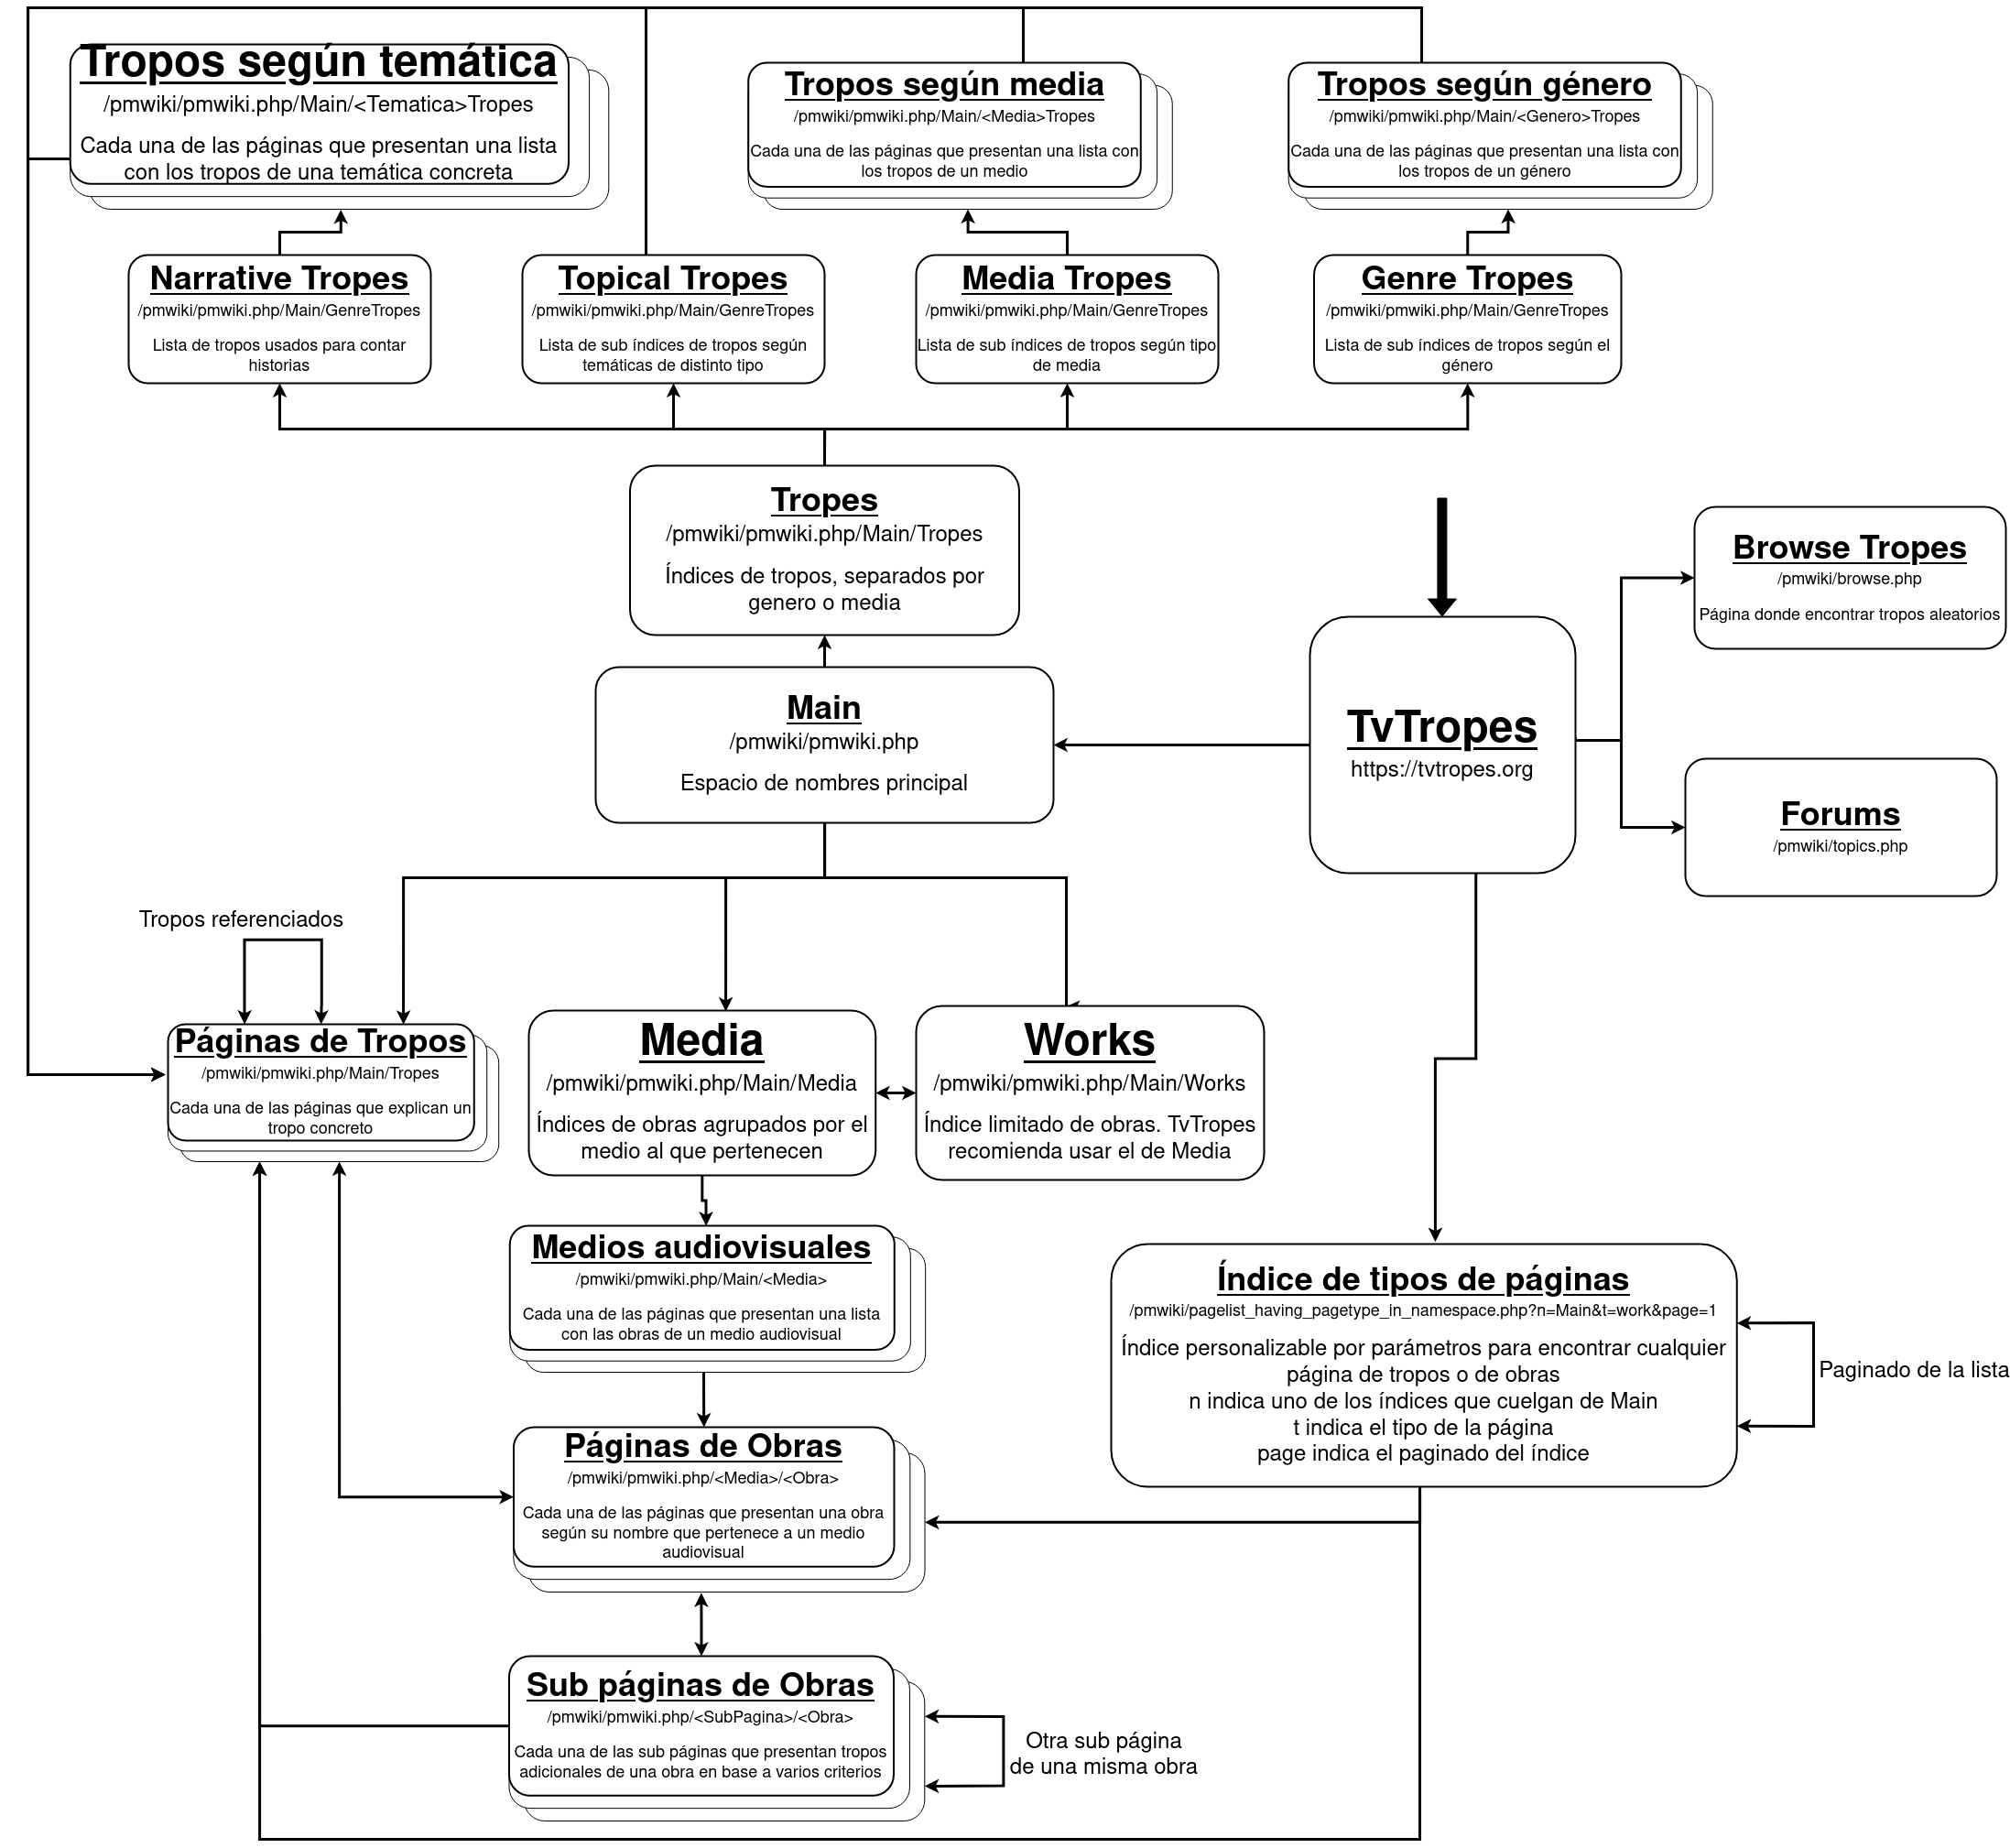
\includegraphics[width=\textwidth]{img/sitemap.png}
  \caption{Mapa del sitio de TvTropes.}
  \label{fig:sitemap}
\end{figure}

Las relaciones más destacables que se pueden observar en el mapa del sitio son
las siguientes:
\begin{itemize}
  \item De \textit{Main} cuelgan la gran mayoría de páginas e índices que debe
  explorar la araña. Existen muchas páginas individuales sin relación entre
  otras y con información que no se han representado al no ser necesaria para
  este trabajo, representando diversos aspectos de la web como la comunidad,
  guías de estilo, información, etc. Estas páginas siguen la misma filosofía que
  las de obras, presentándolas de la misma manera e incluso asociando
  \textit{tropos} a aspectos como el funcionamiento de la propia web, que da a
  ver aún más lo centrales que son estos recursos en esta web.
  \item Existen páginas que, si bien son del mismo tipo, tienen contenidos
  distintos según el contexto, como las páginas de \textit{tropos}, de obras, de
  los distintos índices de \textit{tropos} o de los distintos índices de obras.
  Se han representado como tres rectángulos uno encima de otro para simplificar
  el diagrama, pero todos ellos hacen referencia a que existen muchas páginas de
  esa clase, y no es posible representarlas todas con sus nombres específicos.
  Por ejemplo, la página de una obra dependerá de qué obra represente, y lo
  mismo con los \textit{tropos}. Los índices de \textit{tropos} según temática,
  medio, género o tópico incluyen páginas como \textit{tropos} del género de
  acción o de aventuras, de miedo, de películas, videojuegos o de cualquier otro
  método de organización.
  \item Como se ha explicado antes, existen índices para explorar todos los
  tropos o las obras por tipo de medio. Los índices que aparecen en el mapa del
  sitio, que dependen de \textit{Main}, no son fiables, debido a que no suelen
  contener todas las obras existentes en la web y muchas veces enlazan a índices
  que no tienen que ver. Por ejemplo, es bastante común ir al índice de
  animación asiática y encontrarse con multitud de películas o series que caen
  en la categoría de animación general o en algo completamente distinto como
  animación occidental. Esto hace que sea más fiable saber el índice al que
  pertenece una obra desde dentro de la misma obra y teniendo en cuenta el
  índice principal visto.
  \item Por tanto, el índice más fiable es el que se representa con el nombre de
  índice de tipos de páginas, que es el que se ha visto en la sección anterior.
  Es el más ideal para encontrar todas las páginas porque nos permite listar
  todos los \textit{tropos} u obras según los distintos índices a los que
  pertenecen sin perder ninguno, y navegar hacia cualquiera de ellos, como
  indica la flecha unidireccional. Para navegar dentro del índice hay que tener
  en cuenta que la lista que presenta está paginada, de ahí la flecha de
  navegación hacia sí mismo, ya que, para que la araña explore todo el índice
  debe explorar en profundidad esa página, utilizando el enlace de pasar a la
  siguiente parte de la lista que hay abajo del todo.
  \item Hay relaciones que no se representan al no ser necesarias, como por
  ejemplo que desde la página principal se puede navegar directamente a
  cualquiera de las páginas relevantes de \textit{tropos} u obras, ya sea
  mediante la barra de búsqueda o mediante enlaces que van cambiando
  dinámicamente, ya que, la página destaca cada día nuevas páginas relevantes de
  rápido acceso.
  \item Los \textit{tropos} se están referenciando entre sí constantemente por
  lo que navegar desde uno hacia otro puede ser un proceso interminable. La
  araña puede encontrar otros \textit{tropos} explorando las distintas sub
  páginas de una obra. Las sub páginas, como pueden ser Trivia o YMMV, están
  también representadas como un conjunto genérico, ya que, pueden tomar muchos
  nombres y temáticas. Es importante saber que están siempre enlazadas a la obra
  sobre la que hablan, y no se puede navegar a la de otra obra distinta. Desde
  ellas solo se puede navegar o a otra sub página (siempre de la misma obra en
  la que nos encontramos), a la página principal de la obra o a la página de un
  \textit{tropo} que tiene referenciado en cualquier sub página. Sin embargo,
  cuando desde una página de un \textit{tropo} se referencia a una obra, es
  siempre a la principal.
\end{itemize}

En resumen, desde el índice principal se puede navegar a cualquiera de las
páginas de obras, que pertenecen a un índice de medio audiovisual. Estos medios
audiovisuales se pueden encontrar en el índice principal en \textit{Main}, y
todas las obras están relacionadas únicamente con uno de ellos. Desde la obra se
puede acceder a dos tipos de páginas: sub páginas de la obra y páginas de
\textit{tropos}. Las sub páginas, a su vez, también están relacionadas con los
\textit{tropos}, por lo que se puede navegar hacia ellos desde ahí. Por último,
dentro de una página de \textit{tropos} también se puede navegar hacia otras que
están referenciadas. En general existen una relación casi bidireccional entre
obras y \textit{tropos} al estar referenciándose continuamente. 

\subsection{Estructura de las páginas de TvTropes}
Por último, se analiza la estructura que tiene cada página de TvTropes, tanto de
un \textit{tropo} como de una obra audiovisual, ya sea película, serie,
videojuego, etc. al ser lo que piden las historias de usuario principales
\href{https://github.com/jlgallego99/TropesToGo/issues/6}{[HU01]} y
\href{https://github.com/jlgallego99/TropesToGo/issues/7}{[HU02]}. Se intentan
definir los tipos de páginas más comunes e importantes, pero no todos los que
puedan existir. Es imposible predecir todas las formas que puede tomar una
página, y además eso haría que el \textit{scraper} no supiese adaptarse y fuese
demasiado rígido \cite{nishalscraping}. En general, en esta última sección se
busca identificar las partes más destacables del código HTML de las páginas para
que el \textit{scraper} sepa dónde tiene que buscar la información que necesita
sin redundancia. Este análisis del código HTML se realiza usando las
herramientas de desarrollador presentes en cualquier navegador web, que permiten
observar todo el código HTML de la página, activar o desactivar el JavaScript
para observar los cambios en ella, y demás funcionalidades útiles que sirven en
el ámbito del \textit{scraping} y para sacar conclusiones de las páginas.

Las páginas de obras audiovisuales, independientemente del tipo, se tratan
esencialmente igual y podrían presentar las mismas diferencias que dos del mismo
tipo, sin embargo, suelen tener secciones adicionales. Por ejemplo, si la página
es de una película, es probable que contenga la lista de actores, cosa que por
ejemplo no pasará en un libro o videojuego generalmente, no obstante, en general
entre los cambios que se pueden observar al buscar dos páginas que hacen
referencia a un mismo tema como puede ser dos obras audiovisuales el propósito
es el mismo: describir la obra y sus \textit{tropos}.

Por ejemplo, la página de la serie Los
Soprano\footnote{\url{https://tvtropes.org/pmwiki/pmwiki.php/Series/TheSopranos}}
presenta varias características interesantes, como por ejemplo que el
\textit{tropo}
\begin{otherlanguage}{english}\textit{GenreDeconstruction}\end{otherlanguage}\footnote{\url{https://tvtropes.org/pmwiki/pmwiki.php/Main/GenreDeconstruction}}
no está presente en la sección de \textit{tropos}, que está organizada en cuatro
carpetas según el rango alfabético, sino que se encuentra referenciado en la
propia descripción de la serie. También se pueden encontrar otros
\textit{tropos} que, si bien no están en la propia lista, se les hace referencia
en la descripción de un \textit{tropo} concreto que sí que está en la lista. Al
entrar en otra página, como la de la película El Viaje de
Chihiro\footnote{\url{https://tvtropes.org/pmwiki/pmwiki.php/Anime/SpiritedAway}},
podemos ver que la información ha cambiado por completo de forma y ahora los
\textit{tropos} no se presentan en carpetas y no están organizados por género o
cualquier otra idea, simplemente están en una lista ordenada alfabéticamente.
Por último, es interesante observar una página más, la de la serie
Hannibal\footnote{\url{https://tvtropes.org/pmwiki/pmwiki.php/Series/Hannibal}},
que aunque inicialmente puede parecer que tiene la misma estructura que la de
Los Soprano con cuatro carpetas por rango alfabético, observamos que esos rangos
son distintos. Esta última serie también evidencia otro problema de estructura
que es necesario resolver, y es que existen otras entradas en TvTropes que
también se llaman Hannibal, haciendo referencia o al personaje o a la novela, y
que tienen distinta manera de presentar sus tropos. Sin embargo, cada una de
estas páginas tienen un tipo definido en la web (personaje, serie, libro,
película, etc.) por lo que son más fácilmente identificables.

Como se ha explicado antes, estos cambios estructurales y de organización están
presentes también entre páginas con distintos propósitos, como por ejemplo, en
la página de un \textit{tropo} y de una obra. La página de una obra concreta
muestra los \textit{tropos} organizados en carpetas o listas con distintas
organizaciones, mientras que una página de un \textit{tropo} concreto como el
visto anteriormente de
\begin{otherlanguage}{english}\textit{GenreDeconstruction}\end{otherlanguage} da
la información inversa, es decir, todas las obras que tienen ese \textit{tropo}.
Sin embargo, en este caso la información está presentada de una forma
completamente distinta, esta vez requiere de una mayor exploración a fondo,
puesto que, se dan una serie de géneros con un hipervínculo a sub páginas que
cuelgan de la principal del \textit{tropo} y que ya sí que listan las obras.

En la figura \ref{fig:tvtropes-work} se representan las partes de una página de
una obra en TvTropes que el \textit{scraper} debe saber identificar, ya que
contienen la información que necesitamos. En color azul se muestran las
secciones donde se encuentra información relevante, en verde se muestran las
partes en las que posiblemente se quiera extraer el enlace y/o deban explorarse
más en profundidad y, por último, en rojo se destacan partes no importantes o
que sirven para separar otras que sí son relevantes. Varias de estas partes se
pueden identificar fácilmente en el HTML, puesto que, usan unas etiquetas,
clases e identificadores que siempre son los mismos al ser parte de cómo
funciona internamente la wiki y no contenido que escriben la comunidad. A
continuación se describen estas partes y cómo el \textit{scraper} puede
tratarlas:

\begin{figure}[!h]
  \centering
  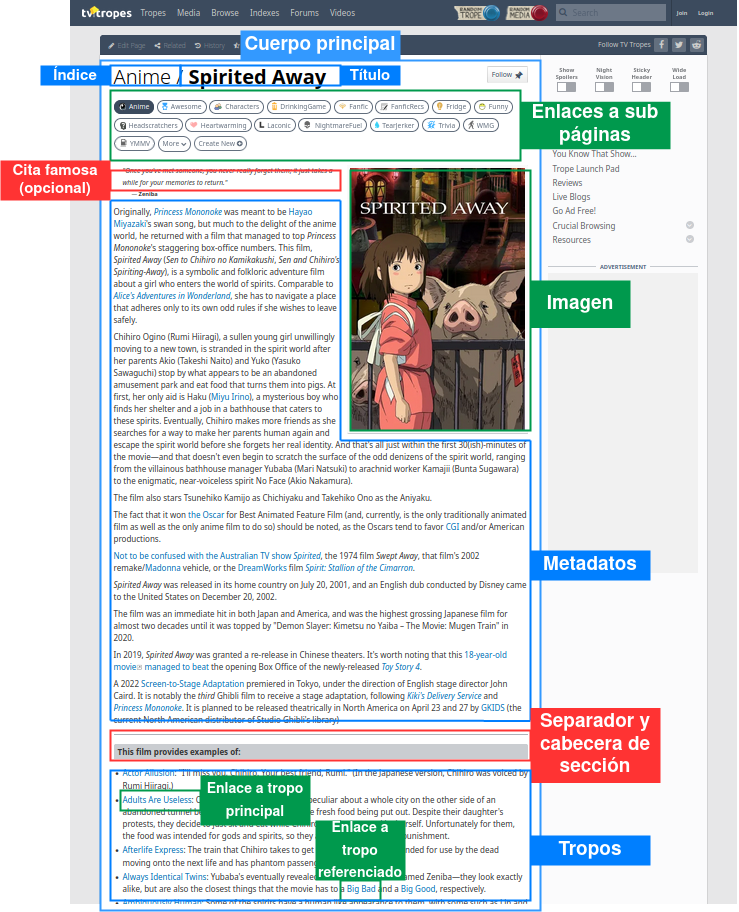
\includegraphics[width=\textwidth]{img/esquema-obra.png}
  \caption{Esquema de las secciones de la página de una obra en TvTropes.}
  \label{fig:tvtropes-work}
\end{figure}

\begin{itemize}
  \item El cuerpo principal es siempre un elemento
  \begin{otherlanguage}{english}\texttt{<article
  id=``main-entry''>}\end{otherlanguage} que nos permite identificar fácilmente
  el cuerpo principal independientemente del tipo de página.
  \item La primera parte del cuerpo principal es siempre una cabecera de sección
  \begin{otherlanguage}{english}\texttt{<h1
  class=``entry-title''>}\end{otherlanguage}. La cabecera contiene en el mismo
  texto el nombre del índice y el título de la obra separados por una barra. El
  nombre del índice siempre está marcado con énfasis, contenido en una etiqueta
  \texttt{<strong>} que lo diferencia del título. Esta diferenciación permite
  conocer a qué índice pertenece cualquier obra.
  \item La sección de enlaces a sub páginas es un poco más compleja; está
  siempre contenida en un elemento de navegación
  \begin{otherlanguage}{english}\texttt{<nav
  class=``body-options''>}\end{otherlanguage} que tiene dentro una lista sin
  ordenar \begin{otherlanguage}{english}\texttt{<ul
  class=``subpage-links''>}\end{otherlanguage}. Dentro de la lista, cada
  etiqueta \texttt{<li>} contiene un hipervínculo a la sub sección de la obra,
  que contendrá otros \textit{tropos} referenciados. En el caso de que una
  página tenga muchos enlaces a sub páginas, no todos se mostrarán directamente,
  y el último botón será un desplegable con el resto. No hace falta usar
  JavaScript para interaccionar con esta parte, ya que, el resto de sub
  secciones que no cabían siguen contenidas ahí. Concretamente, están contenidas
  en el último elemento de lista, que tendrá dentro una etiqueta
  \texttt{<select>} donde cada opción tiene como valor una cadena de texto con
  la ruta URI de la sub página.
  \item A veces, entre las sub páginas y el resumen con metadatos aparece una
  sección con una cita de la obra que se puede ignorar.
  \item Cada obra tiene un resumen, a veces más largo y a veces más corto, que
  cuenta las características principales que tiene. Esta sección es una fuente
  de metadatos difícil de identificar al ser un texto en lenguaje natural, sin
  embargo, también suele contener \textit{tropos} referenciados mediante un
  elemento de hipervínculo. Es posible que parte de los metadatos se encuentren
  separados del resumen, en otro elemento que contenga el texto distinto o
  dentro de una carpeta. Esa carpeta, al igual que con la de \textit{tropos},
  simplemente cambia el texto a visible, por lo que, está en el HTML base y no
  hace falta sacarla de ninguna manera. El resumen está delimitado por un
  elemento \begin{otherlanguage}{english}\texttt{<div
  id=``main-article''>}\end{otherlanguage}, cuyo contenido suele ser muy diverso
  no solo en texto sino en elementos HTML que contiene. Generalmente, los
  distintos párrafos del texto están contenidos en etiquetas \texttt{<p>} o de
  otros tipos. Lo importante aquí es extraer el texto, independientemente de
  dónde esté contenido.
  \item La sección que más interés tiene en cada página de una obra es la de sus
  \textit{tropos}. Antes de esta parte suele aparecer una cabecera que, como se
  vio en \cite{nishalscraping}, tiene un texto que suele cambiar, pero siempre
  suele ser una etiqueta \texttt{<h2>} precedida de una barra horizontal
  \texttt{<hr>} que lo separa del resumen. La sección de los \textit{tropos}
  suele cambiar de forma. A continuación se estudiará más en profundidad cómo
  encontrar los \textit{tropos} en una página de este tipo.
  \item Los marcadores que indican que empieza una sección de \textit{tropos}
  (la línea horizontal y la cabecera) no siempre están presentes. Además, en
  otros casos de páginas, pueden introducir una sección que no contenga
  \textit{tropos}, como pueden ser los actores de una película. En este caso,
  habrá que analizar correctamente las listas e hipervínculos, buscando solo
  aquellos que se sepa que hacen referencia a un \textit{tropo}, que es de la
  página \textit{Main} de TvTropes.
\end{itemize}

En general, los \textit{tropos} pueden aparecer en casi cualquier parte dentro
de la página de una obra y estar organizados de distintas maneras. Algunas los
tienen organizados en una lista o por carpetas en orden alfabético, de géneros o
cualquier otro método de diferenciarlas. También puede haber información de
\textit{tropos} anidada dentro de otros, referenciados en la descripción de la
obra, o incluidos en sub páginas de distinta índole.

En la figura \ref{fig:tropelist} se pueden ver los tres tipos más comunes para
presentar la lista de \textit{tropos} de una obra que se pueden encontrar en
TvTropes. En el primero de la figura \ref{fig:tropelist1} se tiene simplemente
una lista en la cual el primer elemento de cada ítem de la lista es una etiqueta
llamada \texttt{<a class=``twikilink''>} con el nombre del \textit{tropo}, la
clase que ya se ha identificado anteriormente y un enlace a la página de ese
\textit{tropo}. También se puede observar como en la descripción aparecen
enlaces a otros \textit{tropos} que no salen en la lista. El segundo tipo, en la
figura \ref{fig:tropelist2}, es muy parecido al primero solamente que esta vez
están separados en distintas listas, que suelen cambiar el rango alfabético
según la página. Estas carpetas se abren haciendo clic sobre ellas y, mediante
un \textit{script} de JavaScript, aparece la lista de \textit{tropos}, sin
embargo, lo único que hace ese \textit{script} es mostrar la lista modificando
el parámetro CSS de visibilidad. La lista no se inserta dinámicamente, sino que
se pone visible o invisible, por lo que el código HTML base tiene todas las
listas ya definidas independientemente de si están visibles o no. Por último, la
figura \ref{fig:tropelist3} muestra el tipo más complejo y que no es tan común.
Suele aparecer en las obras más famosas, que por lo general tienen un gran
número de \textit{tropos} que hacen que la lista esté contenida en una sub
página y se acceda mediante un enlace en la principal. La dificultad en este
tipo está en que la araña tiene que profundizar en la búsqueda, accediendo a sub
páginas. La ruta de estas será del tipo \texttt{/<NombreDeLaObra>/Tropes<XtoY>}
al final de la URL de TvTropes. En ella, \texttt{<XtoY>} representa un rango
alfabético, siempre precedido por la palabra \textit{Tropes}. Además, estos
enlaces son siempre elementos de primer nivel en la lista, ya que, pueden
aparecer otros que no tienen que ver directamente con los \textit{tropos} y se
pueden ignorar. Una vez entrado en el enlace, la forma de presentar la lista
puede ser de cualquiera de los otros dos tipos vistos.

En el caso concreto de que estén organizados en carpetas, cada una de ellas está
contenida en una etiqueta \texttt{<div>} con un identificador \texttt{folderX}
donde \textit{X} a veces es un número y otras veces puede ser cualquier otra
cosa, generalmente la palabra \textit{label}. En general no siguen una
nomenclatura muy uniforme, pero sí es común que sean etiquetas del mismo tipo y
que empiecen por \textit{folder}. 

Independientemente de cómo se presenten, al final todas las listas que contienen
\textit{tropos} son listas en el lenguaje HTML. Siempre empiezan con una
etiqueta \texttt{<ul>} y cada uno de sus elementos se presentan primero con el
elemento \texttt{<li>} y luego con el enlace que incluye el nombre del
\textit{tropo}. Es bastante usual que, incluso si no están presentados por
carpetas y visualmente parecen una sola lista uniforme, internamente sean varios
elementos \texttt{<ul>} distintos. Las listas siempre están precedidas de una
etiqueta \texttt{<hr>} que pone una línea horizontal y un título \texttt{<h2>}
en el que, como se vio en \cite{nishalscraping}, varía el texto, aunque es
bastante frecuente que contenga las palabras
\begin{otherlanguage}{english}\textit{provides examples of}\end{otherlanguage}.

\begin{figure}[!h]
    \centering
    \begin{subfigure}{\textwidth}
      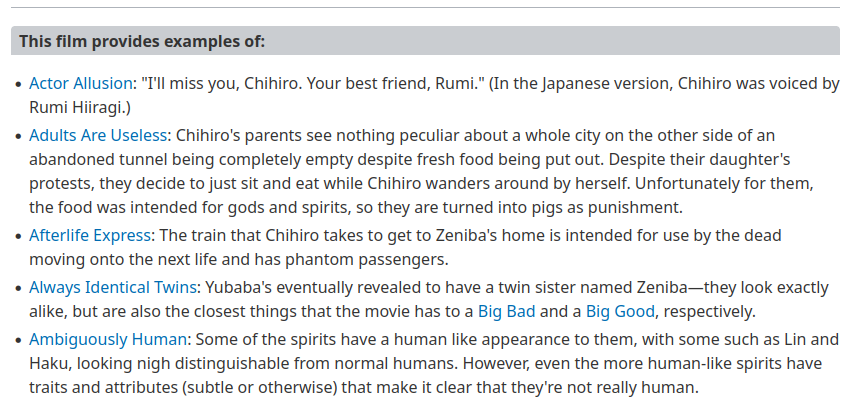
\includegraphics[width=\linewidth]{img/tropes1.png}
      \caption{Lista alfabética de \textit{tropos}.}
      \label{fig:tropelist1}
    \end{subfigure}
    \begin{subfigure}{\textwidth}
      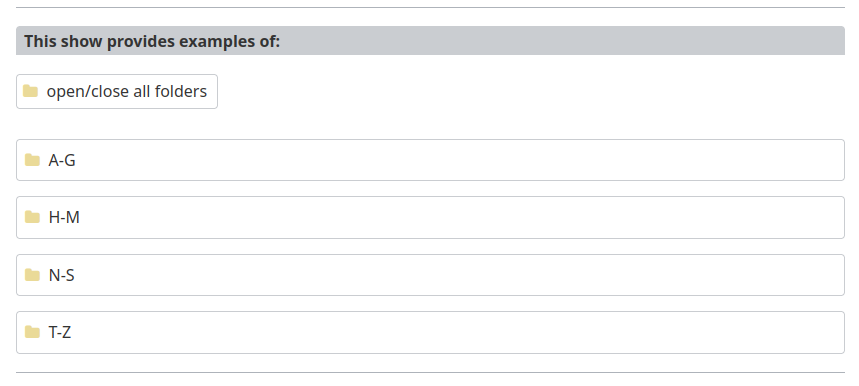
\includegraphics[width=\linewidth]{img/tropes2.png}
      \caption{\textit{Tropos} listados en carpetas.}
      \label{fig:tropelist2}
    \end{subfigure}
    \begin{subfigure}{\textwidth}%
      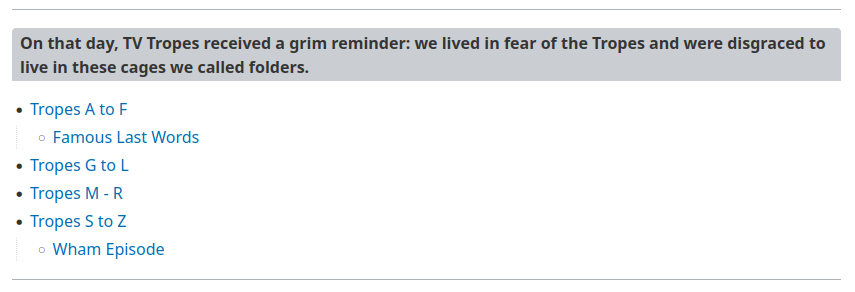
\includegraphics[width=\linewidth]{img/tropes3.png}
      \caption{\textit{Tropos} listados en sub páginas.}
      \label{fig:tropelist3}
    \end{subfigure}
    \caption{Formas más comunes de presentar los \textit{tropos}
    de una obra en TvTropes.}
    \label{fig:tropelist}
\end{figure}

En cuanto a las sub páginas dentro de una obra, estas pueden ser muchas o pocas
según la obra, ya que, también las crea la comunidad. Cualquiera de estas sub
páginas busca dar información interesante relacionada con una obra. En este
caso, están centradas en distintas temáticas o con distintos objetivos y, por
tanto, presentan información que puede ser novedosa. Existen varias muy
frecuentes, como \textit{Laconic}, que da una descripción muy breve de la obra
referenciando varios \textit{tropos} que generalmente no suelen aparecer en la
lista principal, \textit{TearJerker}, que referencia mediante \textit{tropos}
aspectos tristes de la obra, o \textit{Trivia}, que presenta curiosidades sobra
la obra y \textit{tropos} que tienen que ver con esas curiosidades. Otra de las
sub páginas más destacables es la llamada
YMMV\footnote{\url{https://tvtropes.org/pmwiki/pmwiki.php/YMMV/HomePage}}, la
cual contiene otros \textit{tropos} que no toda la comunidad identifica como
correctos o con el mismo significado y, por tanto, no corresponden en la página
principal, que lista los que no tienen diferencias de opinión. Definir todas las
sub páginas de cada obra es imposible, por lo que el \textit{scraper} debe saber
identificar la sección en la que aparecen todas estas páginas, explorarlas y
buscar enlaces de \textit{tropos}. En cualquier caso, en todas ellas la
prioridad es identificar el elemento \texttt{<div>} principal que contiene la
información de la sub página y buscar todas las etiquetas de enlace a
\textit{tropos}. Salvo \textit{Laconic}, que es un pequeño texto, el resto
suelen ser todas siempre del mismo tipo: dos secciones separadas de un pequeño
resumen de la sección (que también incluye referencias a \textit{tropos}) y
varias listas con otros ejemplos nuevos de \textit{tropos}. Esas listas están
separadas generalmente por elementos de \textit{header} que cambian según la
obra, pero donde el \textit{tropo} está incluido en el propio texto y no al
principio de él. Se pueden ignorar los \textit{headers} y simplemente buscar los
elementos de lista. Se puede ver, de forma general, un esquema de cómo son las
sub páginas de una obra en la figura \ref{fig:subpage}.

\begin{figure}[!h]
  \centering
  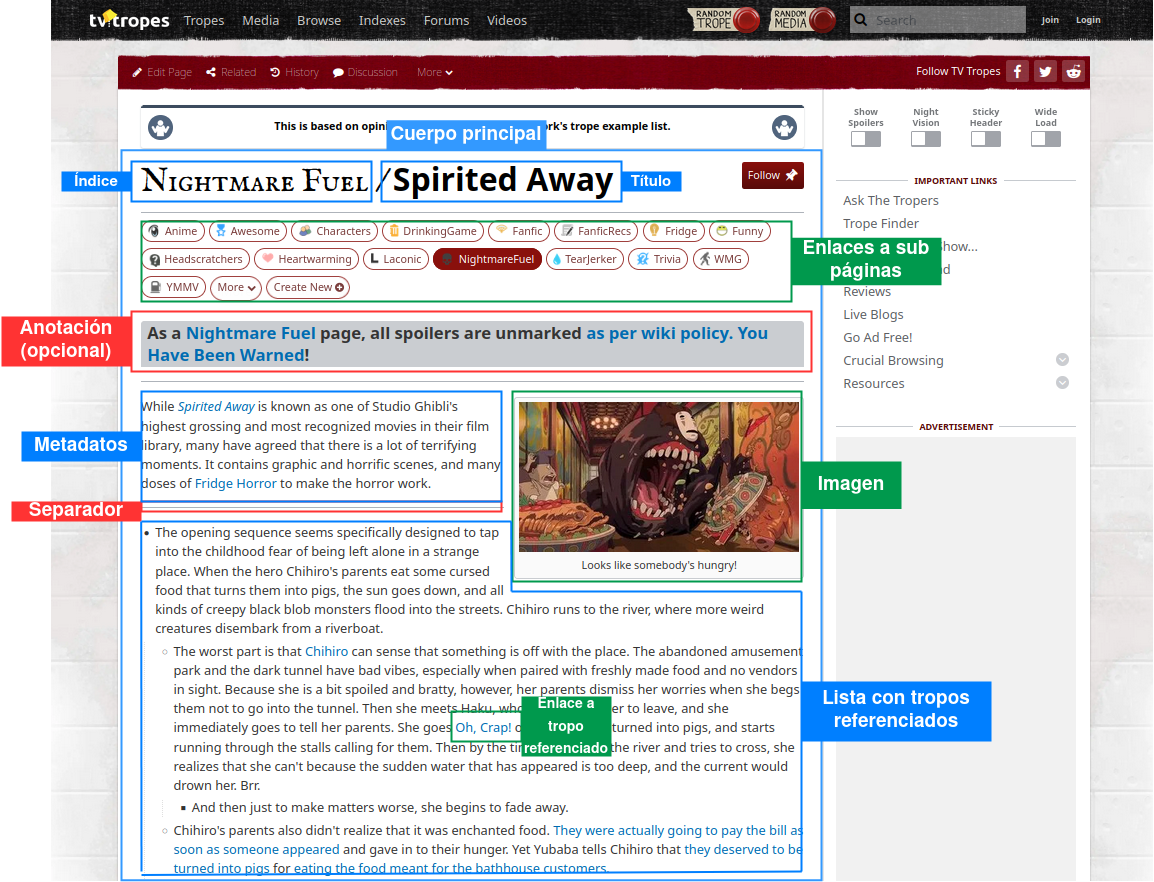
\includegraphics[width=\textwidth]{img/esquema-subpagina.png}
  \caption{Esquema de las secciones de una sub página de una obra en TvTropes.}
  \label{fig:subpage}
\end{figure}

Identificar cuándo se hace referencia a un \textit{tropo}, independientemente de
la página, es sencillo puesto que siempre son hipervínculos con la clase CSS
``\textit{twikilink}'' que, además, siguen el mismo estilo de URL que se ha
visto anteriormente. El \textit{scraper} debe buscar, siempre dentro de la misma
página de la obra, todas las secciones y sub páginas que puedan contener un
hipervínculo de tipo ``\textit{twikilink}'', extraer el nombre del
\textit{tropo} y añadirlo sin repetir.

Finalmente, se resumen los puntos principales que se deducen de este análisis de
TvTropes:
\begin{itemize}
    \item Se considera que todos los \textit{tropos} de una obra audiovisual son
    la suma de todos los que aparecen listados en la página principal, los que
    aparecen referenciados en las distintas sub páginas dentro de la propia obra
    y los que aparecen referenciados en cualquier texto, ya sea el resumen de la
    obra o la descripción de otro \textit{tropo}.
    \item Un \textit{tropo} se identifica al ser una etiqueta HTML \texttt{<a
    class=``twikilink''>}. Su URL es del tipo
    \texttt{https://tvtropes.org/pmwiki/pmwiki.php/Main/} más su nombre en
    estilo \textit{CamelCase}, sin embargo, no todas las páginas con este tipo
    de URL son necesariamente \textit{tropos}.
    \item Existen índices que contienen completamente todos los tropos y obras
    audiovisuales separadas por tipo, listados alfabéticamente y sin confusión
    de pertenecer a cualquier otra categoría. Por tanto, se sabe sin lugar a
    dudas si una página es un \textit{tropo} si está contenido en ese índice.
    \item Se respetarán los nombres que usa TvTropes para almacenar cada obra
    según su tipo de \textit{media}. Extraer dentro de la página de una obra el
    índice al que pertenece permitirá distinguir obras con mismo nombre que son
    de distinto tipo.
    \item La información a extraer en una página de una obra se encuentra
    contenida en el cuerpo principal (figura \ref{fig:tvtropes-work}), punto de
    partida del \textit{scraper}, que contiene varias etiquetas, clases e
    identificadores fácilmente identificables al ser siempre los mismos
    independientemente de la página. De la página de una obra se puede sacar, en
    orden: el índice al que pertenece, su título, un resumen con metadatos y
    \textit{tropos} referenciados, una lista principal de sus \textit{tropos} y
    sub páginas a las que habrá que acceder para identificar otros
    \textit{tropos} listados. Esta información de metadatos sirve para
    satisfacer la historia de usuario
    \href{https://github.com/jlgallego99/TropesToGo/issues/8}{[HU03]},
    eliminando la ambigüedad entre obras, y la historia
    \href{https://github.com/jlgallego99/TropesToGo/issues/9}{[HU04]} y
    \href{https://github.com/jlgallego99/TropesToGo/issues/46}{[HU07]}, para
    saber si la página ha tenido cambios y actualizar los datos.
    \item No es necesario entrar dentro de la página de un \textit{tropo} y
    explorar su código HTML, puesto que, esta solo contiene una descripción de
    este y algunos ejemplos de obras que lo contienen. No es necesario explorar
    esas obras porque ya se encontrarán desde los índices.
    \item No es necesario el uso de un motor de JavaScript en ninguna de las
    páginas, puesto que, toda la información que nos interesa está ya contenida
    en el HTML. En las páginas en las que aparecen contenidos al interaccionar
    con botones o menús desplegables, ese contenido está ya codificado en el
    HTML y el código JavaScript únicamente lo pone visible o invisible.
\end{itemize}

Todas estas características que se han analizado en las páginas de TvTropes
permitirán poder orientar una estrategia de extracción de información con el
\textit{scraper} y que este sepa identificar cuándo una página es extraíble, ya
que sabrá si la estructura de la página que está analizando se adapta a la
información que tiene codificada. Hay que tener en cuenta que todo lo analizado
en este capítulo son generalidades que comparten gran parte de las páginas de
TvTropes. Existen muchas excepciones que se irán encontrando durante el propio
proceso de desarrollo y que se estudiará en el próximo capítulo cómo proceder
con ellas.

	% Desarrollo bajo sprints: 
	% 	1. Permitir registros y login de usuarios
	% 	2. Desarrollo del sistema de incidencias
	% 	3. Desarrollo del sistema de denuncias administrativas y accidentes
	% 	4. Desarrollo del sistema de croquis
	%   5. Instalación de la aplicación de manera automática
	\chapter{Implementación}
\label{chapter:6}

Este capítulo relata el proceso completo de desarrollo del \textit{scraper} para
TvTropes que resuelve los problemas y cumple los objetivos definidos en el
\autoref{chapter:2}. Se siguen uno a uno los distintos hitos que se han ido
alcanzando, explicando por qué son necesarios y las decisiones que se han tomado
en cada uno de ellos para cumplir las historias de usuario, que guían todo el
desarrollo con agilidad.

En este capítulo se irá describiendo el proceso de desarrollo ágil que se ha
llevado a cabo para poder entender cómo se ha llegado a cada uno de los
sucesivos productos mínimamente viables. A lo largo del proceso se justificarán
una serie de decisiones tomadas, buenas prácticas, recomendaciones y
herramientas que permitirán ir refinando el producto hasta llegar a una solución
final de calidad. Esto implica que todos los hitos se desarrollan con el
principal objetivo de satisfacer al usuario y asegurar la calidad, por lo que
conforme se justifiquen las decisiones tomadas para avanzar en cada uno de
ellos, se relacionarán con las historias de usuario definidas, que son las que
confirman qué se debe implementar para cumplir con las expectativas del usuario.

\section{Comienzo del desarrollo}
Con el primer modelado del problema que se ha realizado en el
\autoref{chapter:5}, tenemos definido todo lo necesario para poder comenzar con
el desarrollo y dar una primera versión de un \textit{scraper} que sea capaz de
extraer la información de \textit{tropos} contenida en páginas individuales de
películas de TvTropes. El primer \textit{milestone} de desarrollo es el
\href{https://github.com/jlgallego99/TropesToGo/milestone/3}{M2}, que resuelve
la parte previa a la extracción. Antes de que el \textit{scraper} extraiga la
información que necesita el usuario, que es el objetivo del siguiente hito,
tiene que determinar si la página sobre la que está trabajando es extraíble, es
decir, pertenece a una página de TvTropes que describe una obra con sus
\textit{tropos} y tiene una estructura HTML conocida. Esto permite determinar,
antes de llevar a cabo el proceso de extracción, que el wiki de TvTropes no ha
cambiado demasiado, lo suficiente para saber si el \textit{scraper} programado
sigue funcionando y así evitar procesamiento innecesario. 

Puesto que se está construyendo un producto mínimo, este hito se centra en que
las páginas de obras que se analicen sean solamente de películas, teniendo un
\textit{milestone} futuro dedicado a ampliarlo a otros tipos de medios
audiovisuales. Solo es necesario comprobar y extraer páginas de un tipo de medio
audiovisual concreto para determinar que el \textit{scraper} completa
correctamente sus tareas, ya que el resto de medios consisten en explorar otras
páginas con una estructura similar y que se obtendrán una vez se tenga una araña
que encuentre ese tipo de páginas. Se han elegido páginas de películas por ser
el medio en el que se centran la mayoría de trabajos de investigación estudiados
en la introducción y el estado del arte, y son las que más interés tienen para
una primera versión funcional.

\subsection{Flujo de integración continua para pruebas y compilación}
En este hito se empieza a programar código funcional con lógica de negocio, así
que se comienzan también a desarrollar conjuntamente los tests, concretamente
antes de la propia funcionalidad, tal y como se especifica en el desarrollo
dirigido por pruebas \cite{beck2002driven} y se definió en el
\autoref{chapter:4}. Por tanto, uno de los objetivos de este hito es tener
integrado en el código del proyecto el \textit{framework} de pruebas Ginkgo, que
es el que permitirá desarrollar los tests en Go, para que en los próximos hitos
se puedan desarrollar todas las pruebas para testear las nuevas funcionalidades.
Además, al estar en un entorno de desarrollo ágil la ejecución de las pruebas
estará automatizada, de forma que se tenga un flujo de integración continua que
ejecute automáticamente todos los tests definidos y se pueda comprobar desde el
repositorio de GitHub. 

En cada uno de los hitos, cuando se desarrolla nueva funcionalidad, se abre un
\textit{pull request} en GitHub con los cambios realizados en el proyecto para
saber qué incremento en el producto se está haciendo y qué \textit{issues}
pretende resolver para avanzar en completar el hito. Cada \textit{issue}
representa uno de los sucesivos problemas que surgen durante el desarrollo y que
se intentan resolver para avanzar en completar una historia de usuario. Estos
son los problemas que se justifican y resuelven a lo largo de este capítulo. Los
nuevos flujos de CI que se añaden en este hito permiten automatizar la ejecución
de las pruebas y compilar todo el proyecto, para cumplir que todo el código sea
funcional y asegurar su calidad. Si cualquiera de estos flujos de CI fallan, no
se podrá aceptar el \textit{pull request} y añadir los cambios a la rama
principal. La integración continua en este proyecto se configura mediante
\textit{GitHub Actions}, que automatizan los procesos apoyándose en nuevas
tareas definidas mediante el gestor de tareas \textit{Mask}. Estas tareas
ejecutan los tests para todo el proyecto, ambas usando por debajo la propia
utilidad del lenguaje Go: \texttt{go test} para las pruebas y \texttt{go build}
para comprobar que todos los paquetes del código compilan correctamente. Esto
permite que no haga falta modificarlos en el futuro; servirán para todo el
desarrollo de ahora en adelante y ejecutarán automáticamente todas las nuevas
pruebas que se programen. En el caso de necesitar algún cambio en la ejecución
de los tests o la compilación, bastará con cambiar las tareas del gestor de
tareas, sin necesidad de tocar la configuración de la integración continua.

Por tanto, para poder cumplir con la automatización de las pruebas y la
compilación se configura un nuevo \textit{GitHub Action} en el que se prepara
Go, se instala el gestor de tareas \textit{Mask} y se ejecutan las tareas
definidas para la compilación y el testeo. En un principio se probó a instalar
\textit{Mask} mediante \textit{cargo}, el gestor de paquetes del lenguaje Rust,
ya que la máquina virtual que utiliza el \textit{Action} es de Ubuntu y su
gestor de paquetes no tiene disponible este gestor de tareas en su repositorio
para instalarlo. Sin embargo, esta manera de instalar el gestor de tareas
suponía una gran sobrecarga en el flujo de trabajo al tener que instalar todo el
lenguaje Rust únicamente para instalar un paquete, tardando casi 2 minutos en
ejecutarlo por completo, gastando la mayoría de recursos en instalar el gestor
de tareas. Para solucionar esto se acabó optando por introducir los comandos en
el flujo de CI necesarios para descargar directamente el binario de
\textit{Mask}; esto hizo que se mejorase el tiempo en más de la mitad, ahorrando
los recursos de GitHub y teniendo el resultado del flujo de CI mucho antes.
Adicionalmente, una de las ventajas que tiene el usar Go es que, al ejecutar
cualquier comando de compilación, testeo o ejecución del código, comprueba
automáticamente si las dependencias definidas en el fichero \texttt{go.mod}
están instaladas, y si no lo están las descarga automáticamente, por lo que no
hace falta especificar explícitamente qué dependencias hay que instalar para que
el código funcione.

\subsection{Comprobación de la estructura de una página de TvTropes}
En este hito se modifica el servicio \textit{scraper} añadiendo la funcionalidad
necesaria para cumplir su objetivo: verificar que una página de una obra de
TvTropes no ha cambiado y se puede extraer. Un servicio en DDD hace referencia a
un paquete de código que ejecuta cierta lógica de negocio para un cliente y en
este caso el cliente sería el usuario que necesita los datos. 

El objetivo de este hito se alcanza implementando la función \texttt{CheckValidWorkPage} que 
encapsula la funcionalidad de revisar toda la estructura de una página de
película de TvTropes y validar si el \textit{scraper} podrá extraerla. Recibe
una entidad \textit{Page}, de la cual el \textit{scraper} extrae lo principal
que necesita, que es el URL de la página para poder hacerle una petición y
obtener su código HTML. La razón de recibir la página por referencia se debe a
que la página es mutable, es posible que se haya actualizado y el
\textit{scraper} necesite en el futuro cambiar su atributo de última
modificación, además de que será más eficiente para el \textit{scraper} el
obtener las páginas por referencia que previamente habrá creado el
\textit{crawler} en hitos posteriores. En general, en DDD se tratan las
entidades siempre como referencias, puesto que son mutables, mientras que los
objetos valor se tratarán como variables instanciadas.

Esta función se ha modularizado en distintas subfunciones que realizan
revisiones de distintos tipos, cumpliendo la propiedad de única responsabilidad
de cada una de las funciones y haciéndolas más legibles. Esto facilita que, en
caso de que se necesitasen analizar nuevas partes, se modifiquen las sub
funciones ya existentes o se añada una nueva, que simplemente se llamaría desde
el método principal. Según \textit{clean code} no se deben tener funciones que
mezclen llamadas a otras funciones de alto nivel con lógica más compleja, por lo
que el método principal \texttt{CheckValidWorkPage} se encarga de llamar a las
distintas subfunciones que llevan a cabo verificaciones de distintos tipos y
trata sus resultados para determinar finalmente si la información de la página
es extraíble o no.

Estas comprobaciones se efectúan en orden de menor a mayor complejidad y de
mayor a menor nivel, intentando que el filtrado se lleve a cabo cuanto antes
para evitar entrar en análisis complejos de páginas innecesarias. Se busca poder
validar la página lo antes posible, sin perder mucho tiempo en el proceso para
cumplir la \href{https://github.com/jlgallego99/TropesToGo/issues/45}{[HU06]} lo
mejor posible y que el usuario obtenga cuanto antes el resultado. Primero se
determina si la página pertenece a TvTropes, luego se analiza la estructura
general del artículo principal de la página y finalmente se comprueba la sección
donde deberían estar contenidos los \textit{tropos}.
\begin{itemize}
    \item Para verificar que la página es de TvTropes se extrae el URL de la
    página y se compara si el \textit{host} es \url{tvtropes.org} y si el URI
    corresponde a lo que entendemos como una página de película, es decir,
    pertenece a \textit{Main} y está bajo el índice \textit{Film}. La penúltima
    parte de la ruta tiene que ser el índice al que pertenece la obra, en este
    caso \textit{Film}, y la última parte será el nombre de la película. Esto es
    lo primero que se debe hacer; si la página que se está analizando no es de
    TvTropes y/o no pertenece a una obra, no tiene sentido seguir adelante con
    ella. Sin embargo, puede ser que su estructura interna haya cambiado, por lo
    que es necesario estudiarla más a fondo.
    \item Una vez se sabe que la página es de TvTropes, es necesario ver si
    pertenece a una página de obra y su HTML interno no ha cambiado, ya que es
    de donde luego el \textit{scraper} extraerá la información. Principalmente,
    se revisa en el árbol DOM si la página tiene las partes vistas en el
    análisis de la Figura \ref{fig:tvtropes-work}: un artículo principal con sus
    identificadores y clases conocidas y si el índice, dentro del título del
    artículo, pertenece al de películas. Todas las páginas de obra,
    independientemente de si son películas o no, siguen esta misma estructura,
    por lo que esto basta para confirmar si este tipo de páginas siguen igual.
    \item Por último, se realizan las verificaciones más complejas relacionadas
    con la principal sección que se querrá analizar: la sección de
    \textit{tropos}. Debido al estudio de la Figura \ref{fig:tropelist} del
    \autoref{chapter:5} sabemos que existen tres formas comunes que toma la
    sección de \textit{tropos}, y esto es lo que el \textit{scraper} verifica,
    para asegurarnos de que podemos entender la sección. En este primer hito
    solo se tienen en cuenta los tres tipos, ya que bastan para conformar un
    producto mínimo que sea capaz de analizar la mayoría de páginas de TvTropes,
    sin embargo, en futuros hitos se tendrán en cuenta casos más extremos.\\
    Se sigue la misma estrategia de buscar primero lo más relevante, que en este
    caso es encontrar la sección donde se encuentran los \textit{tropos}, la
    cual está conformada por una lista sin ordenar dentro del artículo principal
    y que está siempre después del resumen y precedida de una etiqueta de
    \textit{header}. Se ignora el comprobar el texto de la cabecera de la
    sección de \textit{tropos}, ya que como se vio en \cite{nishalscraping} el
    contenido cambia mucho y es poco fiable, siendo lo único fiable el hecho de
    que la sección está separada por una cabecera cualquiera. Una vez confirmado
    que la página tiene esa sección, toca ver si se adapta a uno de los tres
    tipos que se conocen. Para probar si los \textit{tropos} están contenidos en
    carpetas basta con buscar el botón de abrir carpetas, que sabemos su
    etiqueta, clase y función JavaScript que utiliza para abrirlas, al estar
    generado siempre igual por el motor del wiki. En todos los casos se valida
    si el primer elemento de la lista es un enlace a una página de
    \textit{tropos} o a una subpágina de ellos. Para este último caso, que
    pertenecería al tercer tipo, se ha hecho uso de una expresión regular que
    confirma si el URI al que redirigen sigue un patrón concreto. Si la última
    parte del URI está codificada como la cadena
    \texttt{/<NombreDeLaObra>/Tropes<XtoY>} entonces se acepta como algo
    conocido. Si la lista contiene cualquier otro elemento inesperado, se
    considera que la página tiene una estructura desconocida y no se puede
    extraer su información.
\end{itemize}

La función de comprobación devuelve un valor booleano, que indica si la página
es extraíble o no, y un error que indica el por qué no es extraíble en caso de
no serlo. En general, es idiomático en Go que todas las funciones devuelvan
siempre un error como último valor para que el código sea autoexplicativo y se
tenga un completo y correcto control de los errores tanto para que las funciones
de testing puedan comprobar todos los casos como para que cualquier cliente que
llame a la función del servicio entienda exactamente qué ha pasado en caso de
error \cite{effective_go}.

Finalmente, en este hito se toma la decisión de que los selectores CSS, los
cuales son una cadena de \textit{string} que hacen referencia a varias etiquetas
HTML y clases, se encapsularán en valores constantes. Esto sigue las guías de
\textit{clean code} sobre evitar los literales, facilitando la legibilidad del
código y evitando la repetición. De este modo, el \textit{scraper} pasará como
parámetro estas constantes a las funciones de Goquery que encuentran los nodos
del árbol DOM de la página que se está explorando. A estas constantes se les da
un nombre lo más semántico posible de forma que el código sea legible y limpio.
Por ejemplo, la constante \texttt{TropeTag} contiene el selector \texttt{a.twikilink} que 
hace referencia a todos los \textit{anchor} de HTML cuya clase es
\textit{twikilink}, que sabemos debido al análisis del capítulo anterior que
hacen referencia a enlaces hacia páginas de \textit{tropos}. El tener constantes
con selectores importantes para lo que quiere buscar el \textit{scraper} también
implica otras ventajas como el poder combinar distintos selectores de modo que
se entienda su significado completo con solo leerlo o el poder adaptarse a los
futuros y posibles cambios que pueda sufrir TvTropes. En el caso de que cambie
alguna clase o etiqueta con la que encontrar alguna sección valiosa de una
página, baste con cambiar la constante y no cambiarlo en cada parte del código
en la que aparezca. En general, al usar constantes semánticas para los
selectores se facilita mucho la legibilidad de algo que de otro modo requeriría
de un análisis más exhaustivo para entender qué significa el selector utilizado,
ya que pueden volverse muy complejos al unir varias reglas.

Se le da en el repositorio de GitHub a esta primera versión del
\textit{software} un etiquetado de versión 0.1.0 que, según las reglas de
versionado semántico\footnote{\url{https://semver.org/}}, hace referencia a que
se añade nueva funcionalidad sin romper lo anteriormente establecido. El primer
número, que indica la versión principal del \textit{software}, se aumentará
cuando se tenga una primera versión completa y funcional de TropesToGo.

\section{Extracción de información en la página principal de una película}
Una vez desarrollada toda la funcionalidad necesaria para comprobar si una
página es de TvTropes y es entendible por el \textit{scraper}, el siguiente paso
lógico es comenzar con el propio proceso de \textit{scraping}, al ser la parte
principal que necesita resolver TropesToGo. La estrategia a seguir en el proceso
de desarrollo es la de centrarse primero en la construcción de uno o más
productos mínimamente viables que culminen en un \textit{scraper} que pueda
sacar toda la información que piden los usuarios según la
\href{https://github.com/jlgallego99/TropesToGo/issues/6}{[HU01]} y
representarlos en un conjunto de datos apto para su uso en procesos de ciencia
de datos, según las historias de usuario
\href{https://github.com/jlgallego99/TropesToGo/issues/30}{[HU05]} y
\href{https://github.com/jlgallego99/TropesToGo/issues/46}{[HU07]}, que
especifican que el usuario necesita acceder al resultado de la extracción en
cualquier momento, de forma offline y en un formato estandarizado. Lo que
produce el \textit{scraper} es el \textit{dataset}; el resultado final que
ofrece TropesToGo al usuario para cumplir sus necesidades, el cual podrá estar
representado en más de un formato ampliamente utilizado por investigadores. Una
vez se tenga un \textit{scraper} totalmente funcional, se podrá avanzar en
futuros \textit{milestones} en el desarrollo de la araña que generalice el
proceso de \textit{scraping} a toda la web de TvTropes completa. 

Por tanto, en este \textit{milestone}
\href{https://github.com/jlgallego99/TropesToGo/milestone/3}{M2} se pretende
ampliar el servicio \textit{scraper} para que pueda extraer los datos presentes
en el artículo principal de varias páginas de prueba. En un principio se tenía
pensado un único hito donde desarrollar el \textit{scraper} completo, capaz de
extraer toda la información necesaria de cualquier película. Sin embargo, al
observar la complejidad que tienen algunas páginas y a lo dispersos que están
los \textit{tropos} de una obra, esa primera idea se dividió en dos productos
mínimos, que son el desarrollado en este hito y en el siguiente. Por tanto, en
este \textit{milestone} el principal objetivo es extraer la información
contenida en la página principal de una película, es decir: su título, año de
salida, índice al que pertenece (el tipo de \textit{media}, o medio audiovisual,
que en este caso será \textit{Film} (película)) y su lista principal de
\textit{tropos}. Existe más información que no se encuentra en el artículo
principal y que se analizará en el siguiente hito, principalmente de
\textit{tropos} adicionales, que está en otras subpáginas de la obra o en
páginas de otros tipos.

Como lista principal entendemos los \textit{tropos} que aparecen directamente
listados al final del artículo, como se podía ver en la figura
\ref{fig:tvtropes-work}, que se consideran los más importantes de la obra al
estar en primer plano. Puesto que este \textit{milestone} está centrado en
extraer información del artículo principal únicamente, se extraerán solo los
\textit{tropos} que están contenidos en listas o carpetas, tal y como se ve en
los dos primeros tipos de la Figura \ref{fig:tropelist}, ignorando por lo pronto
el tercer tipo que, aunque también tiene los \textit{tropos} principales de la
obra, implicaría ahondar en subpáginas. En el próximo \textit{milestone} se
navegará a estas subpáginas y se discutirán las distintas fuentes donde se
pueden encontrar otros \textit{tropos} que no sean los principales.

\subsection{Ampliación del \textit{scraper} para la extracción en el artículo
principal} 

Antes de desarrollar la funcionalidad del \textit{scraper} ha sido necesario
construir la factoría encargada de crear los objetos \textit{Media}, cada uno de
los cuales representa toda la información de una obra de cualquier medio
audiovisual de TvTropes, incluido sus \textit{tropos}. El patrón factoría es uno
de los recomendados en \textit{Domain Driven Design} para la creación de
agregados, y se encarga de formar correctamente el objeto para cumplir la
propiedad de única responsabilidad. Es imprescindible poder generar este tipo de
objetos correctamente, ya que los utilizará el \textit{scraper} para rellenarlos
con los datos extraídos. Por supuesto, de la mano de la creación de la factoría \texttt{Media} 
vienen los tests necesarios, que prueban con varios objetos
válidos e inválidos para comprobar que se cumplen todos los casos definidos y el
manejo de errores es correcto. La factoría, como es común en Go, gestiona una
serie de errores que devuelve como segundo argumento para asegurar siempre que
se conoce el estado de lo que devuelve cualquier método.

En cuanto a la implementación de los métodos que amplían el \textit{scraper}
para darle la funcionalidad de extracción de datos sobre una página web de
TvTropes, se ha seguido una estrategia muy parecida a la seguida en el
\textit{milestone} anterior y según las guías de código limpio
\cite{clean_code_rules}. Se tiene un método principal de \textit{scraping},
encargado de extraer la información relevante de una página de TvTropes
individual, con una separación clara entre la función de alto nivel y las sub
funciones de más bajo nivel a las que llama, encargadas de analizar y extraer
datos de distintas partes de la página.

En general, en el ámbito del \textit{scraping} las tres herramientas más
imprescindibles son: los selectores CSS, que dan operaciones y reglas para
encontrar rápidamente elementos en el HTML de una
página\footnote{\url{https://developer.mozilla.org/es/docs/Web/CSS/CSS_Selectors}};
las expresiones regulares, para identificar patrones y poder tratar mejor las
cadenas de texto fruto de aplicar un selector CSS; y, por último, las
herramientas de desarrollo del navegador web, para analizar el HTML interno de
una página, encontrar las partes fundamentales que se quieren extraer y probar los
selectores CSS en ella para comprobar que apuntan justo a los recursos deseados.

Para extraer el título, el índice y el tipo de medio audiovisual de la página de
una obra (en este caso, solo obras que son películas) se han empleado los mismos
selectores que en la comprobación de la página y que se vieron en el análisis de
la estructura de TvTropes, que apuntan directamente al \textit{header} del
artículo que tiene toda esta información. En este caso, puesto que queremos la
información y no basta con verificar, se ha hecho uso de una expresión regular
que separa las tres partes que queremos, que es capaz de identificar cualquier
año en mitad de una cadena de texto. Sin embargo, el principal problema a la
hora de extraer información en el artículo principal ha estado relacionado con
los \textit{tropos}. En un principio se tenía ideado el extraer solamente los
\textit{tropos} que figuran en la lista, como cabeza de cada uno de los
elementos de ella, y también aquellos a los que se hace referencia en las
descripciones de ellos y en el resumen de la película. El problema de esto es
que se han encontrado casos de \textit{tropos} que, cuando están referenciados
en mitad de un texto y no como un elemento principal de la lista, no pertenecen
necesariamente a la obra. En algunos casos se referencian como ejemplo de
\textit{tropo} contrario o cualquier otra razón, lo que hace que no se pueda
determinar si pertenecen como tal a la obra o no, así que se descartan. Por
tanto, se hace un cambio de estrategia en el que se considera que, para este
\textit{milestone}, los \textit{tropos} que se extraen son únicamente los que
aparecen en cada elemento de la lista o carpetas, que se consideran
``principales''.

Ha sido necesario construir dos selectores CSS nuevos, apoyándose en las guías
de Mozilla para selectores, que permitan seleccionar fácilmente y de manera
exclusiva los \textit{tropos} principales, tras un proceso de análisis de la
página mediante el inspector de elementos HTML del navegador. Cada uno de estos
selectores condensan en una sola instrucción todo lo necesario para encontrar
cada uno de los enlaces a \textit{tropos} que encabezan cada elemento de la
lista, tanto para una lista simple como para el caso de que estén en carpetas.
Como se vio en la figura \ref{fig:tvtropes-work}, cuando TvTropes define los
\textit{tropos} de una obra, siempre los muestra en una lista donde cada primer
elemento es un hipervínculo con estructura conocida y fácilmente identificable.
Por supuesto, al igual que en el hito anterior, se construyen los selectores
como \textit{strings} constantes con un nombre legible, de forma que se eviten
utilizar literales en el código y sea más legible.

Por tanto, se obtienen inequívocamente los \textit{tropos} de una lista simple
en el artículo principal de una obra de TvTropes mediante el selector CSS de la
Figura \ref{fig:selector-lista}.

\begin{figure}[ht]
    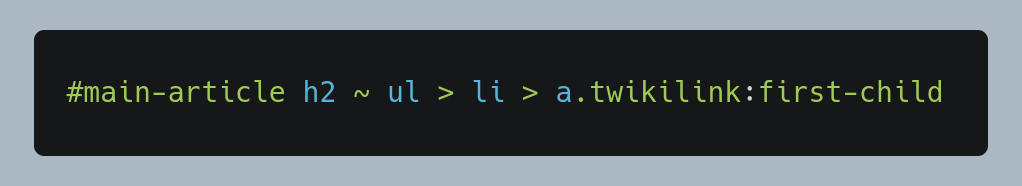
\includegraphics[width=\textwidth]{img/selector-tropes.png}
    \caption{Selector CSS para extraer todos los \textit{tropos} principales de
    la lista simple.}
    \label{fig:selector-lista}
\end{figure}

La primera parte es común en otras funciones del \textit{scraper}, ya que busca
el artículo principal, que es donde siempre va a estar toda la información que
necesitamos, y luego busca el \textit{header} que siempre precede a la sección de
\textit{tropos} independientemente de la página. Una vez hecho esto, se hace uso
del combinador general de hermanos
\begin{otherlanguage}{english}(representado por el símbolo
\textasciitilde)\end{otherlanguage} para seleccionar los elementos HTML que
están al mismo nivel; en este caso, identifica todos los primeros elementos de
lista \texttt{<ul>} que son hermanos de la cabecera que da inicio a la sección
de \textit{tropos}. Se recuerda que, aunque visualmente en la página parezca una
sola lista, internamente suele estar partida en distintos elementos \texttt{<ul>} 
al mismo nivel, por lo que esto nos permitiría seleccionar todos
ellos. Con esto ya tenemos identificada sin lugar a equivocaciones la sección de
\textit{tropos}. A continuación, se emplea dos veces el combinador de hijo
\begin{otherlanguage}{english}(representado por el símbolo
\textgreater)\end{otherlanguage}, que escoge aquellos elementos que sean hijos
directos del primer elemento. Partiendo de que se tiene seleccionada la lista
principal, en la primera combinación se buscan todos sus hijos directos, que son
cada uno de los elementos \texttt{<li>} de la lista, y en la segunda se busca el
siguiente hijo directo, que es la primera etiqueta que encabeza cada punto de la
lista. Esta etiqueta es ya el hipervínculo al \textit{tropo} que queremos. Al
final, se indica la pseudo clase \texttt{:first-child} para indicar que
únicamente queremos el primer enlace de \textit{tropos} \texttt{a.twikilink} que
aparezca. De esta manera se ignoran aquellos enlaces que no queremos, que son
los que aparecen referenciados en la descripción de cada \textit{tropo}
principal, y solo nos quedamos con el que encabeza cada punto de la lista.

Este selector completo también resuelve uno de los principales problemas que se
han encontrado al intentar extraer los \textit{tropos}. Existen muchos casos en
los que un elemento de la lista de \textit{tropos} contiene sublistas con
descripciones adicionales y \textit{tropos} que no queremos, al ser
referenciados en la descripción y no principales. En primeras versiones del
selector se llegaba a meter en esas sublistas, sin embargo, se pudo resolver
gracias al combinador general de hermanos, que únicamente selecciona las listas
que estén al mismo nivel, evitando meterse en sublistas. 

En cuanto al selector para los \textit{tropos} que se encuentran en carpetas, en
la \ref{fig:selector-folder}, es muy parecido al anterior pero con una ligera
diferencia necesaria. Aunque dentro de las carpetas lo que se tenga es una
estructura HTML idéntica al caso en el que no haya carpetas, distintos elementos \texttt{<ul>} separados 
arbitrariamente donde cada elemento es un \textit{tropo}, el que es hermano de
la cabecera de la sección de \textit{tropos} en este caso no es un elemento \texttt{<ul>} sino 
la carpeta. Por eso, en este caso, el selector se simplifica,
buscando únicamente los hijos directos de la carpeta, sin necesidad del selector
de hermanos. Esto también evita las sublistas, porque no son hijos directos de
la carpeta.

\begin{figure}[ht]
    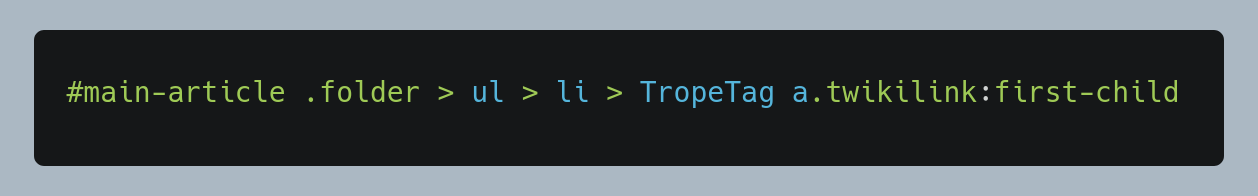
\includegraphics[width=\textwidth]{img/selector-tropes-folders.png}
    \caption{Selector CSS para extraer todos los \textit{tropos} principales en
    carpetas de listas.}
    \label{fig:selector-folder}
\end{figure}

El resultado final de ambos selectores es, por tanto, todas las etiquetas de
hipervínculo que indican un \textit{tropo} principal. Estas tienen los dos datos
necesarios para el \textit{scraper}: el nombre del \textit{tropo}, dentro de la
propia etiqueta, y su URI en el elemento \texttt{href} para poder dirigirse a
esa página si fuese necesario.

Con esto ya estaría desarrollada la parte del \textit{scraper} correspondiente a
este hito, que se encarga de extraer toda la información de una página y
construir el objeto con la información de la página con sus \textit{tropos}.
Cabe destacar que para implementar la estructura de datos que maneja los
\textit{tropos} de una obra se ha utilizado un set, ya que es una estructura de
datos en la que todos sus elementos son únicos, y en una obra no tiene sentido
que existan \textit{tropos} repetidos. Finalmente, se desarrollan sin problema
los tests que comprueban que el resultado de la extracción es correcto,
comprobando si el título, año y URL son los esperados y si en el set todos los
objetos hacen referencia a \textit{tropos} reales y no están repetidos. Estos
tests se realizan con varias páginas de TvTropes de prueba que tienen los
\textit{tropos} en listas y en carpetas. Una vez hecho esto, el próximo paso
para completar este hito es poder trasladar esta información a un
\textit{dataset}.

\subsection{Implementación de repositorios para manejar los \textit{datasets}}
Finalmente, la última parte que resta para completar este hito es el
almacenamiento de uno o varios objetos \texttt{Media} en un conjunto de datos
con un formato estandarizado. Recordamos que estos objetos son agregados que
representan una obra con sus \textit{tropos}. Los repositorios son los
encargados en DDD de persistir los agregados y, como se vio en el modelado
inicial del problema, se modela un repositorio para este tipo de objetos.

En la interfaz repositorio de \texttt{Media} se describen únicamente aquellos métodos
genéricos que cumplan las necesidades del usuario. La principal funcionalidad es
la de poder añadir objetos \texttt{Media} al \textit{dataset}, ya que según la
\href{https://github.com/jlgallego99/TropesToGo/issues/6}{[HU01]} y la
\href{https://github.com/jlgallego99/TropesToGo/issues/30}{[HU05]}, el usuario
quiere la totalidad de los datos extraídos en un único \textit{dataset}, y que
según la \href{https://github.com/jlgallego99/TropesToGo/issues/46}{[HU07]}
quiere poder tenerlo en cualquier momento, por lo que tiene que ser un conjunto
de datos persistido en memoria, en un fichero al que pueda acceder. Además de
esto, también se debe poder actualizar el conjunto de datos debido a la
naturaleza cambiante de los datos en TvTropes, y el usuario pide tener la
versión más reciente de la información, tal y como indica la
\href{https://github.com/jlgallego99/TropesToGo/issues/9}{[HU04]}. Por otro
lado, métodos que suelen ser típicos de implementaciones CRUD, como la lectura
del repositorio, no tienen sentido que las ofrezca el \textit{scraper}. El
usuario no va a utilizar este \textit{software} para leer los datos, sino para
que le genere un conjunto con ellos que ya utilizará en la manera que crea
necesario y, por tanto, solo son necesarias funcionalidades de creación, borrado
y actualización.

Esta definición genérica de la interfaz repositorio permite poder implementar en
cualquier momento \textit{structs} que, implementando todos los métodos de la
interfaz, definan una nueva forma de persistencia de los datos extraídos. Esto
garantiza la propiedad de extensibilidad del código y está en consonancia con la
\href{https://github.com/jlgallego99/TropesToGo/issues/30}{[HU05]}, donde se
especifica que el usuario quiere poder elegir el formato en el que se represente
el conjunto de datos de entre los más comunes en ciencia de datos. El
representar los repositorios del conjunto de datos como algo genérico, con una
misma definición, permite tener en cuenta en todo momento esta historia de
usuario para añadir nuevos formatos soportados por TropesToGo en caso de
necesitarlos y luego poder reutilizarlos fácilmente. Para seguir esta HU y
cumplir este hito, se implementan dos repositorios de \texttt{Media} para
\textit{datasets} en formato CSV y JSON. El formato CSV es el más frecuente en
cualquier tarea de ciencia de datos y tiene la ventaja de que es independiente
del lenguaje. Por su parte, el JSON tiene las mismas ventajas, estando presente
en multitud de ámbitos como formato para representación de datos, como por
ejemplo en API REST, y es el formato de los datos de Tropescraper.

En cuanto a la información que tiene que contener el \textit{dataset}, ya la
conocemos, puesto que son todos los campos que contiene cada objeto \texttt{Media} 
en los que, sin embargo, la forma de representación varía entre
los formatos de datos. En general, en el fichero de datos tienen que figurar una
serie de entradas, una detrás de otra, que representen una obra y toda su
información relevante. Esta información es: tanto el título como el año de la
obra, para identificarla inequívocamente
(\href{https://github.com/jlgallego99/TropesToGo/issues/8}{[HU03]}), su URL de
TvTropes, la fecha en la que se actualizaron sus datos por última vez, el tipo
de medio audiovisual al que pertenece (para este hito, de momento solo
películas) y su lista de \textit{tropos}, donde cada \textit{tropo} es una tupla
de su nombre y su índice. 

El índice al que pertenece un \textit{tropo} hace referencia al tipo o
papel que tiene en la narrativa de una historia; pueden ser narrativos, de
género, sobre temas específicos, etc. y es una decisión guiada por la
\href{https://github.com/jlgallego99/TropesToGo/issues/57}{[HU08]}. El usuario
necesita esta información para poder realizar análisis más complejos en los que
se entiendan las relaciones entre \textit{tropos} al conocer de forma objetiva
para qué se utilizan. La extracción de esta información no se hace en este
hito, se delega a un \textit{milestone} posterior, ya que es información de
metadatos secundaria que no es imprescindible para construir este producto
mínimo, sin embargo, el hecho de que exista se tiene en cuenta desde el
principio.

Los repositorios para JSON y CSV se implementan en paquetes separados, para
preservar el principio de única responsabilidad, y definen únicamente las
funciones necesarias. Por tanto, se tienen módulos de repositorio completamente
desacoplados, que únicamente reciben un objeto \texttt{Media} con el cual
efectuar sus operaciones. Se puede ver un ejemplo de cómo estaría representada
la información completa de una obra en la Figura \ref{fig:json-dataset} para el
\textit{dataset} JSON y en la Figura \ref{fig:csv-dataset} para el conjunto de
datos CSV. En el caso de JSON se tiene una clave principal ``tropestogo'', que
contiene un array con todos los resultados del \textit{scraping}. Cada uno de
los objetos contiene toda la información principal en el mismo nivel, y los
\textit{tropos} son un array cuya información anidada contiene su título y su
índice. En el fichero CSV cada dato es una columna, sin embargo, para
representar los tropos y sus índices se ha tenido que separar en dos columnas
distintas. Dentro de esas columnas se tiene de igual manera un array, donde cada
elemento está separado por punto y coma (un delimitador distinto que el que
separa entre columnas, que es la coma), y la posición en un array se corresponde
con la del otro, para relacionar el nombre del \textit{tropo} con su índice.

\begin{figure}[ht]
    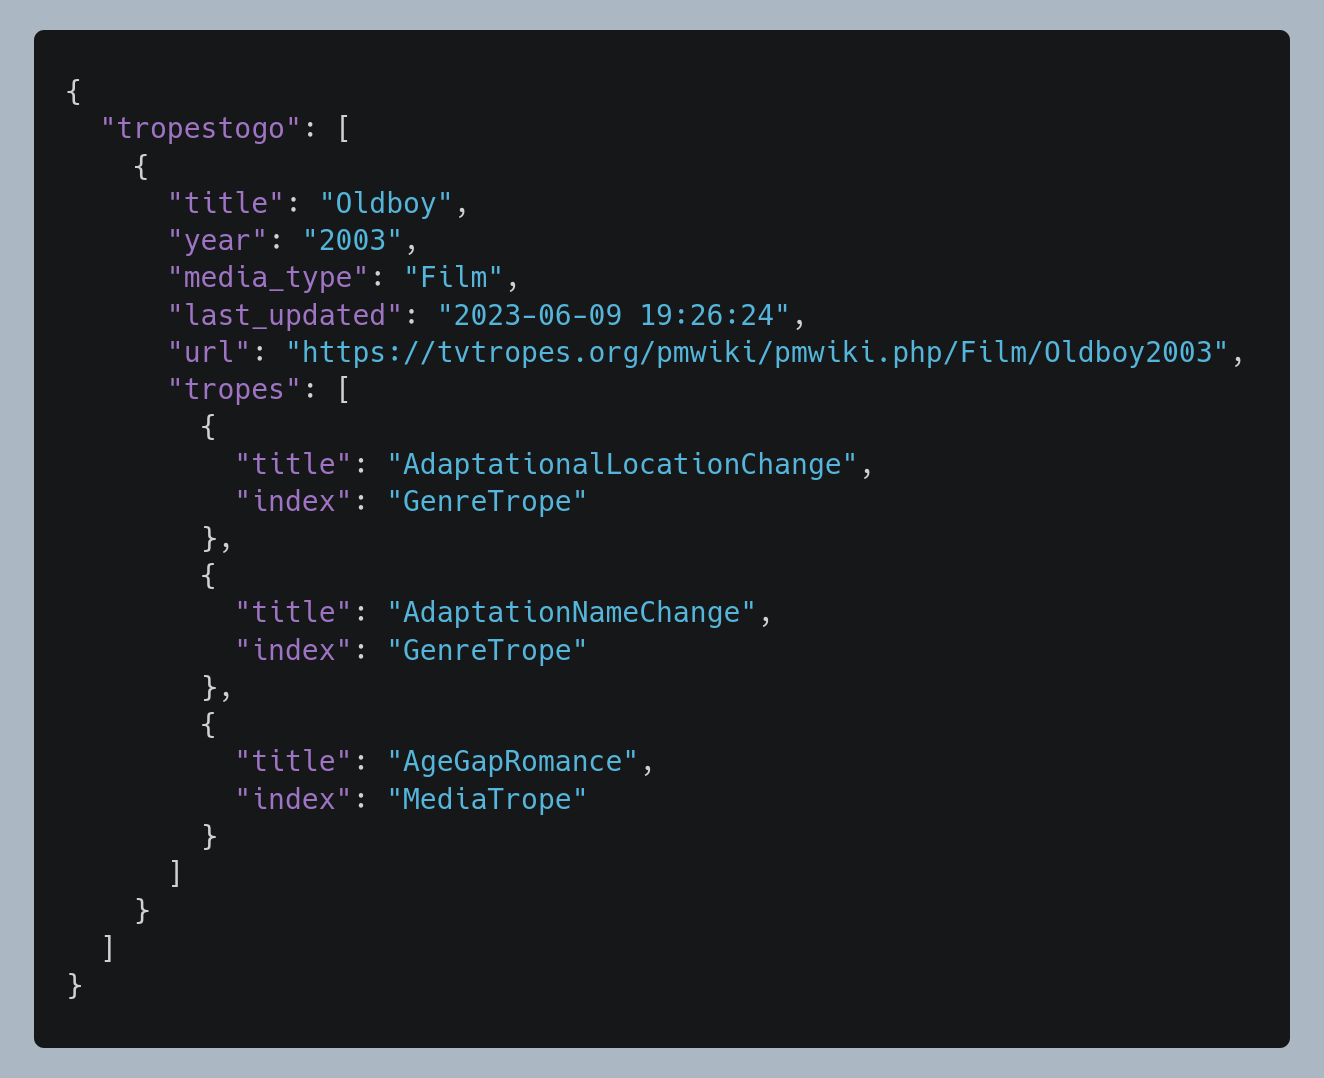
\includegraphics[width=\textwidth]{img/dataset-json.png}
    \caption{Ejemplo de representación de los datos de una película de TvTropes en JSON.}
    \label{fig:json-dataset}
\end{figure}

\begin{figure}[ht]
    \begin{table}[H]
        \begin{tabular}{|l|l|l|}
        \hline
        title         & year & lastupdated         \\ \hline
        Oldboy (2003) & 2003 & 2023-06-09 19:26:24 \\ \hline
        \end{tabular}
    \end{table}
    \begin{table}[H]
        \begin{tabular}{|l|l|}
        \hline
        url                                                    & mediatype \\ \hline
        https://tvtropes.org/pmwiki/pmwiki.php/Film/Oldboy2003 & Film      \\ \hline
        \end{tabular}
    \end{table}
    \begin{table}[H]
        \begin{tabular}{|l|}
        \hline
        tropes                                                        \\ \hline
        AgeGapRomance;AdaptationalLocationChange;AdaptationNameChange \\ \hline
        \end{tabular}
    \end{table}
    \begin{table}[H]
        \begin{tabular}{|l|}
        \hline
        tropes\_index                    \\ \hline
        MediaTrope;GenreTrope;GenreTrope \\ \hline
        \end{tabular}
    \end{table}
    \caption{Ejemplo de los campos que tiene un \textit{dataset} de TvTropes en CSV.}
    \label{fig:csv-dataset}
\end{figure}

Para tratar con los ficheros en JSON ha sido necesario implementar la interfaz
\textit{Marshaler} de la biblioteca estándar de Go, ya que es obligatorio si se
quieren codificar y descodificar objetos complejos a JSON. Con esto ya se tiene
una forma sencilla de transformar objetos entre el fichero JSON y las
estructuras internas del código. En el caso de CSV es más sencillo debido a que
la biblioteca estándar de CSV de Go contiene una función para escribir sobre
este tipo de ficheros. En general, el CSV es más fácil de tratar, puesto que es
un formato muy sencillo que consta únicamente de líneas una detrás de otra, más
fáciles de tratar con los métodos convencionales de escritura y lectura de
ficheros. 

Se sigue una misma estrategia en ambos repositorios para facilitar la gestión de
los datos y para reducir lo máximo posible el número de lecturas y escritas en
ficheros, que pueden comprometer bastante la eficiencia (en relación con la
\href{https://github.com/jlgallego99/TropesToGo/issues/45}{[HU06]}). El flujo
general de funcionamiento de los repositorios consiste en que, al añadir un
nuevo objeto \texttt{Media} correctamente formado, no se persiste directamente,
sino que se almacena en un vector de objetos \texttt{Media} como parte del
objeto \textit{scraper}. Este vector se va rellenando con las sucesivas llamadas
de añadir objetos \texttt{Media} hasta que finalmente se decida llamar a un
método que se encarga de volcar (persistir) todos los datos de la variable en
memoria al fichero, vaciando la memoria y construyendo todo el \textit{dataset}
en una sola vez.

Los métodos de borrado y actualización siguen una filosofía muy parecida en
ambas implementaciones. El borrado se ha implementado como una limpieza completa
del dataset, para ayudar en la regeneración de conjuntos de datos al testear,
eliminando todo registro, tanto en memoria como en el \textit{dataset}, y
dejando únicamente la cabecera de las columnas en el CSV o la clave principal
con un array vacío en el JSON. La actualización por su parte consiste en un
proceso de carga de todo el \textit{dataset} del fichero en una variable
temporal, lo cual permite tratar más fácilmente los datos en términos propios
del lenguaje. Para esto, en el caso de JSON basta con realizar una
decodificación del JSON a las estructuras de datos de Go que contienen los
datos, haciendo la actualización como una búsqueda simple en el array de objetos \texttt{Media} 
y modificando lo necesario. Al llevar a cabo las modificaciones sobre los
objetos internos, se vuelve a escribir todo el conjunto de datos, terminando la
actualización. Este es un proceso que está pensado solamente en el caso de que
el \textit{scraper} encuentre datos más actualizados, para no tener que volver a
generar todo el conjunto, sino únicamente actualizar el objeto que se quiere.

Por su parte, el añadir datos nuevos consiste únicamente en añadir de forma
intermedia el objeto \texttt{Media} al vector en memoria, comprobando
previamente que no es repetido, quedándose ahí hasta que se decida persistirlo.

Adicionalmente, en este hito se ha tomado la decisión de replantear un poco el
modelado DDD de las páginas de TvTropes. Modelar una única página como una
entidad es insuficiente para hacer relaciones correctas y tiene más sentido como
un objeto valor que, además de su URL, que es lo principal, describa también qué
tipo de página de TvTropes es. Saber si la página es de una obra, \textit{tropo}
o índice permitirá al \textit{scraper} y al \textit{crawler} en el futuro
trabajar de una manera más rápida y sencilla. Ahora, para representar todas las
páginas de TvTropes, se utiliza una entidad \texttt{TvTropesPages} que se
encarga de gestionar la creación y mantenimiento del conjunto de todas las
páginas encontradas en TvTropes, donde el objeto valor \texttt{Page} es el
identificador de cada página, que están relacionados directamente por hash (en
una estructura \textit{map}) con su fecha de última actualización. Esta entidad
controla la creación de las páginas y da la posibilidad de modificar su fecha de
actualización. 

Por último, a lo largo del desarrollo de este \textit{milestone} se detecta un
problema importante que es necesario resolver para terminar este PMV: los tests
del \textit{scraper} del hito anterior funcionaban haciendo peticiones HTTP
directamente a TvTropes. Esto interfiere directamente con cómo deberían ser las
pruebas unitarias, que deberían únicamente confiar y usar los recursos
propios del proyecto. Que los tests dependan de si TvTropes está funcionando, de
la velocidad de la red, o incluso de arriesgarse a ser vetado de la página o con
peticiones limitadas por tiempo, puede dificultar los tests de la lógica interna
del \textit{scraper}, que deben poder ejecutarse y funcionar independientemente
de si TvTropes está disponible en ese momento o no.

Para resolver esto, se realizan pequeños cambios en el planteamiento del
\textit{scraper}, dejando el análisis de la página como una subfunción de la
que recibe una entidad página y realiza una petición HTTP a TvTropes. A partir
de ahora se emplearán, únicamente para los tests, ficheros HTML descargados
directamente de TvTropes y guardados en el repositorio. Esto supone una
consideración adicional que ya se discutió en el \autoref{chapter:3}; los
contenidos de TvTropes están bajo una licencia
\begin{otherlanguage}{english}\textit{Creative Commons
Attribution-NonCommercial-ShareAlike 3.0
Unported}\end{otherlanguage}\footnote{\url{https://CreativeCommons.org/licenses/by-nc-sa/3.0/}},
la cual permite redistribuir sus contenidos siempre que sea de forma no
comercial, con la misma licencia y dando crédito al autor original. Puesto que
descargar y trabajar directamente con el HTML de algunas páginas TvTropes entra
dentro del uso de esta licencia, se añade al repositorio de GitHub, se informa
de su uso y se da crédito a TvTropes como los autores de ese contenido.
 
Ahora el análisis de una página de TvTropes trabaja directamente sobre cualquier
objeto genérico que contenga el HTML de la página, siendo el cómo se obtiene ese
objeto un paso previo que se queda encapsulado en una función previa que realiza
peticiones HTTP y llama a esta función de análisis. Por tanto, los tests pueden
directamente llamar a esta función de análisis cargando desde el test el fichero
HTML que se tiene en disco. Esta nueva manera de enfocar los tests nos permite
evitar los problemas de red poder testear más en profundidad los contenidos de
una página, ya que al estar persistida en disco sabemos que no va a cambiar, y
confirmar así que la lógica del \textit{scraper} es correcta.

Se le da en el repositorio de GitHub a esta nueva versión del \textit{software}
un etiquetado de versión 0.2.0 que, según las reglas de versionado
semántico\footnote{\url{https://semver.org/}}, hace referencia a que se añade
nueva funcionalidad sin romper lo anteriormente establecido. En general, lo que
se hace es aumentar y mejorar la funcionalidad del \textit{scraper}.

\section{Extracción de información en las subpáginas de una película}
En TvTropes las páginas se organizan en espacios de nombres, y uno de esos
espacios de nombres son las sub
wikis\footnote{\url{https://tvtropes.org/pmwiki/pmwiki.php/Main/SubWiki}}, o sub
páginas de una obra, que presentan información más centrada en un tema concreto.
Cada obra tiene una serie de subpáginas temáticas muy variadas; no todas tienen
las mismas, pero siempre se hacen referencia en ellas a \textit{tropos} que, en
muchos casos, no están en la parte principal. En muchos casos estos
\textit{tropos} se consideran demasiado subjetivos y dependen del criterio del
miembro de la comunidad que los ha identificado, como por ejemplo los del
espacio de nombres YMMV. Por estas razones, podemos hacer una distinción entre
los \textit{tropos} de una obra que son principales, al estar listados en el
artículo principal, y secundarios, al pertenecer a una o más subpáginas
temáticas dentro de una obra. A continuación, se resuelve el segundo producto
mínimamente viable relacionado con la extracción de \textit{tropos} de una obra,
que tendrá ya el desarrollo mínimo de un \textit{scraper} para TvTropes con el
que poder pasar a trabajar en la araña. Por tanto, en este hito se abordará el
proceso de desarrollo y ampliación del \textit{software} para la extracción de
\textit{tropos} en subpáginas. Esto aumentará el número de \textit{tropos} que
TropesToGo es capaz de identificar, organizando cada vez más la información tan
distribuida que tiene TvTropes. Todo este desarrollo sigue motivado
principalmente por la
\href{https://github.com/jlgallego99/TropesToGo/issues/6}{[HU01]}, que nos pide
obtener todos los \textit{tropos} de todas las obras de la web, y se tendrá una
solución que mejore la extracción que realizaba Tropescraper, que se centraba
únicamente en los \textit{tropos} principales.

\subsection{Ampliación del \textit{scraper} para extraer todos los \textit{tropos} principales en subpáginas}
Antes de pasar a la extracción en los subwikis, es necesario ampliar el
\textit{scraper} con lo último necesario para que sea capaz de obtener los
\textit{tropos} principales de todo tipo de páginas. En el hito anterior se
obtuvieron aquellos ordenados en cualquier tipo de lista o carpetas, y quedaba
por ver el último tipo de la Figura \ref{fig:tropelist} en el que, cuando los
\textit{tropos} principales son demasiados, se dejan fuera del artículo
principal y es necesario explorar subpáginas que los dividen y ordenan
alfabéticamente.

Estas subpáginas con \textit{tropos} principales siempre siguen las mismas
reglas, que han facilitado su extracción:
\begin{itemize}
    \item Los enlaces a ellas se encuentran siempre donde está la sección de
    \textit{tropos}. En este caso, la lista contiene únicamente enlaces a sub
    páginas de diversos tipos, pero no necesariamente principales, sino también
    temáticas con \textit{tropos} secundarios. En la Figura \ref{fig:tropelist3}
    se puede ver un ejemplo de esto, donde se dan enlaces a dos subwikis
    distintas de lo principal. 
    \item Se identifica cuándo un enlace es a una subpágina de \textit{tropos}
    principales con una simple expresión regular que compruebe que las dos
    últimas partes del URI son: primero, el título de la obra, y segundo, una
    cadena del tipo
    \begin{otherlanguage}{english}``TropesXtoY''\end{otherlanguage}, donde X e Y
    son cualquier letra mayúscula, que indican el rango alfabético de
    \textit{tropos} que presentan.
    \item La estructura de cada una de estas subpáginas es idéntica a la de una
    página típica de obra, solo que únicamente conteniendo la parte de
    \textit{tropos}.
    \item Los \textit{tropos} se presentan en cualquiera de las dos formas
    vistas anteriormente: listas o carpetas, con el \textit{tropo} principal
    encabezando cada elemento de la lista.
\end{itemize}

Por tanto, para realizar esta extracción se ha utilizado una estrategia simple
reutilizando el método que extrae los tropos del anterior milestone. Este método
era capaz de, como sabemos, extraer todos los tropos presentes en cualquier
artículo principal siempre que estuviesen en listas o carpetas. Puesto que esta
misma estructura de a veces carpetas a veces listas. Por tanto, para solucionar
esto basta con lanzar esta función general de tropos tantas veces como sub
páginas se encuentren, formando listas parciales de \textit{tropos} por cada sub
página y formando una lista final sumando todas ellas. Ahora, cuando el
\textit{scraper} extrae información de una página de obra y llega a la sección
de \textit{tropos}, comprueba si estos están en subpáginas o no, y según eso
sigue una de las dos estrategias.

\subsection{Responsabilidad única del \textit{scraper} y uso de \textit{readers}
para testing} 

Adicionalmente, se llevan a cabo varios retoques del servicio \textit{scraper}
para hacerlo más funcional, que sus métodos estén más centrados en una única
funcionalidad y en general tener el código más limpio, claro y documentado.

Para poder tener un producto mínimo viable más adecuado, y garantizar la propiedad de
única responsabilidad del \textit{scraper}, se vuelve a dar un pequeño
cambio, pero importante, a la entidad \texttt{TvTropesPages} que modela todas las
páginas que se encuentren en TvTropes. El \textit{scraper} debe encargarse
únicamente de extraer información de páginas que se le ofrezcan, es decir, la
responsabilidad de buscar las páginas y sus subpáginas no recae en él, sino en
el \textit{crawler}. Todas las funciones del \textit{scraper} deben, por tanto,
trabajar con esta entidad o con objetos valor página de forma individual,
únicamente sacando datos, formando objetos \texttt{Media} correctos y manejando
sus repositorios (los \textit{datasets}) para que los clientes hagan lo
pertinente con ellos.

Se crea una entidad \texttt{TvTropesSubpages} que relaciona mediante un
\textit{map} una serie de subpáginas con sus respectivas fechas de última
actualización para satisfacer la
\href{https://github.com/jlgallego99/TropesToGo/issues/9}{[HU04]}. De igual
manera, para poder modelar cada página con sus subpáginas, se relacionan
mediante un \textit{map} en la entidad \texttt{TvTropesPages} cada página
(objeto valor \texttt{Page} que representa una página de cualquier tipo), con la
entidad de las subpáginas. De esta manera, se modela una entidad que
gestiona y relaciona todas las páginas, sus subpáginas y las fechas de última
actualización de todas ellas. Esta es la principal entidad con la que se quiere
que trabaje el \textit{crawler}, al encontrar las páginas que luego se quiere
que extraiga el \textit{scraper}.

Adicionalmente, se modifican todos los métodos de extracción para que trabajen
con objetos \textit{reader} de la biblioteca de entrada/salida de Go. Un
\textit{reader}\footnote{\url{https://pkg.go.dev/io}} representa cualquier flujo
de datos de lectura, y es el tipo de datos que acepta Goquery para formar el
árbol DOM con el que trabaja el \textit{scraper}. La ventaja de definir los
parámetros de las funciones del \textit{scraper} como \textit{readers} es que el
contenido HTML puede venir de cualquier fuente, ya sea de haberlo obtenido tras
una petición HTTP o de leer un fichero local en disco. Por tanto, ahora se tiene
un método general que se encarga de realizar todas las llamadas a los distintos
métodos que hacen el \textit{scraping} de las distintas partes de una página,
para todas las páginas, pero donde el reader es el HTML obtenido de hacer una
petición HTTP a TvTropes. Para los tests, se llama directamente a cada uno de
los métodos para testearlos, dándoles como parámetro un \textit{reader} con el
contenido de la página HTML que se tiene guardada en disco, para seguir
garantizando que los tests funcionen en cualquier ámbito y sin depender de
factores externos.

Esto conforma una nueva versión del \textit{software} funcional, con 0.3.0 como
número de versión, indicando que ha habido una mejora con nueva funcionalidad.
Concretamente, esta nueva funcionalidad es la posibilidad de extraer
\textit{tropos} principales en subpáginas.

\subsection{Extracción general de \textit{tropos} en los subwikis para todos los espacios de nombres}
Previo a esta extracción, se modifica el objeto valor \texttt{Trope} para
reflejar dos nuevos campos: si es principal y, si no lo es, a qué subwiki (o
espacio de nombres) pertenece. Esto pone de manifiesto aún más la ventaja de
tener los \textit{tropos} modelados como objetos valor, ya que pueden
representar más sencillamente estos campos. Puesto que los objetos valor son
inmutables y se instancian, un mismo \textit{tropo} puede estar instanciado dos
veces en dos obras distintas, porque en una puede ser principal y en otra no,
por ejemplo. En general, los \textit{tropos} se modelan como algo que siempre
nos dice lo mismo, pero siempre dentro del contexto de cada obra. Este modelado
nos permitirá organizar y representar mejor los \textit{tropos} que se extraen
con esta ampliación del \textit{scraper}.

El \textit{scraper} no debe realizar ninguna tarea de \textit{crawling}; sus
métodos reciben páginas y subpáginas en la que todo lo que necesita es la URL
para acceder a ellas y buscar datos. Por tanto, su cometido es extraer toda la
información de \textit{tropos} de cualquiera de las subpáginas que reciba,
tanto de \textit{tropos} principales como de subwikis. Para poder reflejar el
nuevo cambio en la representación del objeto \textit{tropo}, el \textit{scraper}
debe comprobar en qué tipo de subpágina está. Esto se hace con una simple
comprobación mediante expresiones regulares como ya se vio en la sección
anterior con las subpáginas de \textit{tropos} principales. En este caso, los
subwikis tienen siempre las dos mismas partes al final del URI: el espacio de
nombres y el título de la película. Por tanto, basta con una simple extracción
del espacio de nombres del título de la página y validar si la forma del URI
coincide. El \textit{scraper} construirá el \textit{tropo} como principal o
secundario en relación con la página de donde los esté extrayendo, y al crearlo
indicará el espacio de nombres al que pertenece.

El conjunto de todos los \textit{tropos}, como se vio en el modelado del
problema, se implementa mediante un set, que garantiza que todos sus elementos
son únicos. Existe la posibilidad de que un mismo \textit{tropo} aparezca en dos
espacios de nombres distintos, y esto no se considera como duplicado, ya que
aunque el título de este sea el mismo, el espacio de nombres no lo es, por lo
que son dos elementos distintos. Esto permite que los \textit{tropos} tengan más
información interesante que pueda permitir relacionarlos entre sí, siguiendo la
\href{https://github.com/jlgallego99/TropesToGo/issues/57}{[HU08]}, y en general
garantizar la propiedad de que los \textit{tropos} existen dentro de un
contexto.

La entidad \texttt{Media} es la encargada de formar la película con toda su
información, por lo que también se encarga de organizar las listas de
\textit{tropos} en dos categorías: principales y secundarios. Estos
cambios también se reflejan en los \textit{datasets} JSON y CSV, añadiendo un
nuevo \textit{array} para los \textit{subtropos} en el JSON y dos nuevas
columnas en el CSV, que representan respectivamente todos los sub
\textit{tropos} y todos los espacios de nombres de ellos.

La estrategia a seguir para la extracción en subwikis es muy parecida a la
seguida en la parte anterior. Se lanza el método de \textit{scraping} general de
\textit{tropos} por cada uno de los subwikis, con la diferencia de que en este
caso los \textit{tropos} están ordenados de formas muy diversas. Los
\textit{tropos} principales se suelen presentar en los tipos vistos, pero en los
subwikis es más común ver mucho texto y pocos \textit{tropos}, que generalmente
no están ni ordenados en listas ni carpetas; en general depende mucho de la sub
wiki. Por esta razón, se ha seguido una estrategia de extraer cualquier
referencia que aparezca en cualquier parte del artículo principal de la sub
wiki, por supuesto siempre comprobando que lo que se extrae es efectivamente un
\textit{tropo}. Este hito, además, ha motivado la simplificación de los métodos
de \textit{scraping} de las páginas y de garantizar su única responsabilidad y
encapsulamiento. Se ha podido reducir su funcionamiento a lo más importante,
teniendo ahora un método de extracción de \textit{tropos} que funciona para
cualquier tipo de página, dependiendo del selector CSS elegido. El
\textit{scraper} simplemente recibe todas las subpáginas y determina el
selector más adecuado para cada una de ellas, realizando todo el proceso de
extracción con una interfaz única y sencilla que facilita la reutilización y
ampliación a más casos, algo imprescindible al diseñar para una página tan
cambiante como TvTropes.

Con este incremento, en el que además se termina este PMV por completo, se tiene
la versión 0.4.0, en la que finalmente se tiene una versión bastante completa
del \textit{scraper}. TropesToGo es ahora capaz de extraer cualquier tipo de
\textit{tropo}, tanto principal como secundario, que aparezca en la página de
una obra y todas sus subpáginas asociadas. Por tanto, se tiene un
\textit{scraper} lo suficientemente completo como para satisfacer en gran medida
lo pedido en la
\href{https://github.com/jlgallego99/TropesToGo/issues/6}{[HU01]}, por lo que
los siguientes esfuerzos de desarrollo se centrarán en ampliar el
\textit{scraping} a un mayor número de páginas. Es decir, el siguiente paso es
el desarrollo del \textit{crawler} o araña, que permitirá evolucionar el
\textit{software} para que, en lugar de extraer páginas individuales, llegue a
extraer y representar la información de todas las películas de TvTropes.

\section{Desarrollo de la araña}
Teniendo desarrollada la funcionalidad que permite extraer todos los datos
de cualquier página de película y asociarla con varios metadatos y
\textit{tropos}, el próximo paso es poder aplicar esa funcionalidad de
extracción a todas las películas y sus \textit{tropos} que han sido registrados
en TvTropes. Según la
\href{https://github.com/jlgallego99/TropesToGo/issues/6}{[HU01]}, el usuario
necesita obtener todas las obras posibles, lo que le permitirá poder realizar
estudios más completos y actuales al tener un mayor conjunto de datos. Para
poder conseguir esto es necesario desarrollar otro componente esencial en la
extracción de datos en páginas web: el \textit{crawler} o araña.

El principal objetivo de este \textit{sprint} de desarrollo es el de dar una
versión mínima y funcional de un \textit{crawler} que opere concretamente con lo
pedido en este problema; debe ser capaz de encontrar todas las páginas
relevantes de TvTropes para que el \textit{scraper} pueda extraer, limpiar y
persistir sus datos. Para garantizar la separación entre los dos servicios, y la
única responsabilidad de cada uno, el \textit{crawler} se ocupa únicamente de
buscar URL valiosos, construir el objeto \texttt{Page} correcto y almacenarlo
en la entidad \texttt{TvTropesPages} sin ninguna tarea de extracción
de metadatos, ya que no es su cometido. El \textit{scraper} únicamente necesita el
contenido HTML de cada página para buscar los datos necesarios, contenido al que
accede gracias a conocer previamente las páginas de las que lo tiene que
extraer.

El \textit{crawler} debe mantenerse simple en su implementación, para dar una
versión con todo lo necesario para avanzar, pero siendo lo suficientemente
escalable para poder ampliarlo en función de si fuese necesario. Esto es algo
esencial en el ámbito del \textit{scraping}, y más en una página como TvTropes
en la que sus contenidos son muy complejos y están distribuidos en múltiples
lugares; se pueden encontrar nuevas fuentes de datos o páginas que
requieran de un \textit{crawling} adicional. En línea con los objetivos de este
trabajo y las historias de usuario planteadas, su principal objetivo debe ser el
de conseguir todas las páginas importantes de TvTropes de la forma más eficiente
posible, ya que será la parte de todo el \textit{software} que tratará con un
mayor volumen de datos. Adicionalmente, se deben tener muy en cuenta los
aspectos éticos y de eficiencia del \textit{scraping}, porque en este punto del
desarrollo se comienza a trabajar con un gran número de páginas de una web que
no queremos sobrecargar ni que nos limite o deniegue el acceso, lo que
imposibilitaría completar el desarrollo.

\subsection{Estrategia general para la búsqueda y extracción de todas las páginas relevantes de TvTropes}
El \textit{crawler} es el segundo servicio que se implementa en TropesToGo. Un
servicio implica una unidad de \textit{software} con una funcionalidad concreta
y encapsulada que pueda trabajar individualmente, sin embargo, su último fin
en el contexto general de este trabajo es funcionar junto al servicio
\textit{scraper} para dar un resultado final que cumpla las necesidades de los
usuarios. El \textit{crawler} primero buscará e indexará todas las páginas en
una entidad común, utilizable por cualquier cliente del \textit{crawler}. Ese
cliente será el \textit{scraper}, que usará esas páginas para extraer los datos
y generar el \textit{dataset} con el resultado final. 

Tener el \textit{crawler} y el \textit{scraper} como dos servicios separados que
funcionarán en conjunto permite poder modificarlos sin afectar al resto del
código, algo imprescindible al resolver un problema de este tipo, ya que como
nos indica la \href{https://github.com/jlgallego99/TropesToGo/issues/9}{[HU04]}
TvTropes es muy propensa a cambiar. En general, esta es la filosofía que se
sigue a lo largo del desarrollo; todos los artefactos del código (los dos
servicios, los repositorios para los \textit{datasets} o las entidades que
representan los datos de TvTropes) están encapsulados en distintos paquetes que
se pueden modificar sin propagar errores al resto, haciendo muy sencilla la
escalabilidad.

Las páginas relevantes dependen de la información que se quiera y de dónde se
obtenga. Una buena estrategia de \textit{crawling} tiene que tener en cuenta un
buen punto de partida y cómo encontrar desde ahí exactamente el tipo de páginas
que necesita. No es necesario extraer cualquier URL, ya que pueden resultar
inútiles y ocupar espacio en memoria innecesario, además de dificultar el propio
proceso de extracción. En nuestro caso, el principal objeto son las películas (y
más adelante, cualquier obra), aquellas de dónde luego el \textit{scraper}
extraerá toda su información: metadatos y \textit{tropos} asociados.

En la figura \ref{fig:crawling} se puede ver un diagrama de flujo que detalla la
estrategia que se sigue para encontrar y extraer todas las páginas de
TvTropes que queremos; en este primer caso, todas las películas, pero en el próximo hito se
ampliará para cualquier otro medio audiovisual que presente obras con
\textit{tropos}. Esta estrategia está basada en el algoritmo básico de
\cite{olston2010web} modificado y aplicado a este problema en concreto. Las
características principales de este proceso son las siguientes:
\begin{itemize}
    \item La estrategia de extracción en TvTropes en este incremento consiste en
    la indexación de páginas y subpáginas de obra, es decir, aquellas que están
    en un espacio de nombre distinto a \textit{Main}, que es el de
    \textit{tropos}. Cada espacio de nombres corresponderá a un tipo de medio
    audiovisual. La mayoría de los \textit{tropos} están presentes en la página
    principal de la obra y/o en cualquiera de sus subpáginas.
    \item Se utilizan como semillas todas las páginas del índice estudiado en el
    \autoref{chapter:5}, el cual es un script interno de TvTropes que nos
    asegura encontrar todas las páginas del espacio de nombres que se le
    indique. Para este hito, se indica el espacio de nombres \textit{Film}, en
    el que se encuentran las películas. El \textit{crawler} encuentra en ese
    índice las páginas principales de obra, para luego profundizar en la
    búsqueda dentro de cada una de esas páginas buscando cualquier enlace a sub
    páginas de cualquier tipo.
    \item Una vez extraídos y almacenados los URL de cada página en una
    variable intermedia, se construye y se añade el objeto \texttt{Page} a
    la entidad \texttt{TvTropesPages} final que conformará el resultado del
    \textit{crawling}. Se comprobará al añadir cada obra si se ha alcanzado el
    límite para detener el proceso o no.
\end{itemize}

\begin{figure}
    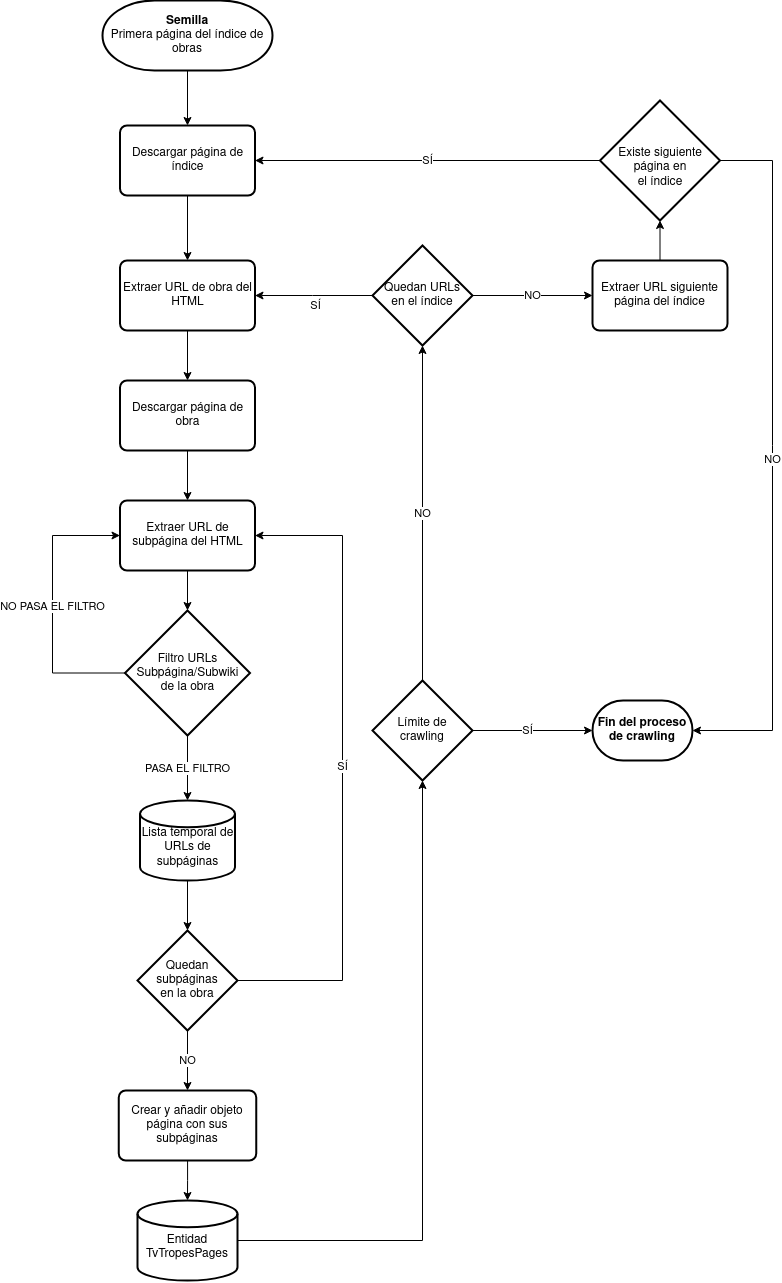
\includegraphics[width=\textwidth]{img/flujo_crawler.png}
    \caption{Diagrama de flujo del funcionamiento del \textit{crawler}.}
    \label{fig:crawling}
\end{figure}

Esto mejora la estrategia de Tropescraper, que encontraba las páginas de
películas a través de referencias en las de \textit{tropos}. En TvTropes no se
puede confiar que una página, de cualquier tipo, liste todos los ejemplos
relacionados. Existen numerosos casos de películas que tienen un \textit{tropo}
concreto, pero que luego no aparecen referenciadas al entrar en la página de ese
\textit{tropo}. Esta relación bidireccional a la cual se ha hecho alusión
en ocasiones anteriores no siempre es cierta, porque aunque técnicamente estén
relacionados, no se puede esperar que los redactores humanos de TvTropes hayan
tenido en cuenta todas las relaciones y referencias en ambas direcciones y las
hayan escrito. Con este índice no solo se mejora por completo el
\textit{crawling} de TvTropes, asegurando que se obtienen todas las obras
registradas sin lugar a duda, sino que simplifica enormemente el proceso al
estar todo organizado en un índice. Además, el \textit{scraping} de Tropescraper
solamente extraía los que están en la sección principal, ignorando los subwikis.

Con este desarrollo se produce un incremento en el valor del producto, teniendo
ya un \textit{crawler} de TvTropes completamente funcional para cumplir
principalmente la
\href{https://github.com/jlgallego99/TropesToGo/issues/6}{[HU01]}. Se libera con
esto una versión 0.5.0 de TropesToGo, ya que se añade nueva funcionalidad sobre
el mismo API.

\subsection{Limitación de la carga al servidor de TvTropes}
Como se ha introducido al inicio de este hito, llegados a este punto del
desarrollo es imprescindible tener en cuenta ciertas cuestiones relativas a la
relación entre el bot y la página web y empezar a seguir varias políticas de
cortesía en la implementación. El objetivo es tener una ejecución más eficiente
y que suponga una carga mínima sobre TvTropes, realizando solamente las
operaciones necesarias y sin repetir nada ya extraído, lo cual es imprescindible
al estar ya trabajando con grandes volúmenes de datos. Esto además limitará el
riesgo de que TvTropes ejerza mecanismos anti-\textit{scraping}, como pueden ser
el retraso de peticiones, la denegación de acceso temporal o, lo que sería aún
peor, bloquear el acceso por completo. Se necesitan de mecanismos que permitan
que el programa funcione como un usuario más sin llamar la atención.

Todo este proceso de mejora del \textit{crawler} se basa en las
\href{https://github.com/jlgallego99/TropesToGo/issues/7}{[HU02]} y
\href{https://github.com/jlgallego99/TropesToGo/issues/45}{[HU06]}, que nos
indican que el usuario quiere poder obtener los datos de la forma más rápida
posible y pudiendo elegir no tener la totalidad de los datos existentes. Como
paso previo, se permite elegir limitar el proceso de \textit{crawling} a un
número de obras limitado en lugar de encontrarlas todas. Esto facilitará la
creación de demos y satisfará a aquellos usuarios que necesiten solo de un
subconjunto reducido de los datos, que además reducirá enormemente el tiempo que
el bot tenga que estar trabajando.

\subsubsection{Reutilización de páginas extraídas}
Con la primera versión del \textit{crawler} construida, se realizó una pequeña
demo real sobre TvTropes para comprobar su efectividad. Se consiguieron extraer
más de 500 películas, sin embargo, pasado ese umbral el programa paró de dar
resultados. Al entrar a TvTropes desde un navegador se pudo ver la razón: la web
mostraba una única página con un mensaje indicando que TvTropes detectó un
número alto de peticiones y que esperase unos pocos minutos antes de volver a
intentarlo de nuevo, lo cual puso de manifiesto la necesidad de controlar mucho
mejor las peticiones HTTP enviadas.

Una de las principales razones por las que se llegó a este caso se debía a que
el \textit{crawler} necesita extraer el HTML, teniendo que llevar a cabo, por
tanto, una petición HTTP a la página para ello. Y luego el \textit{scraper}, que
solo tenía los URL de las páginas encontradas por el \textit{crawler}, volvía a
repetir peticiones a esas páginas para volver a obtener sus contenidos, por lo
que cada página de obra se llamaba dos veces, sobrecargando la red más de lo
necesario.

Existen varias soluciones para esto, que pasan por la idea de tener una caché
(temporal o persistida) de los contenidos de las páginas extraídas. Esto se
puede hacer de múltiples maneras: mediante variables en el código,
descargándolas y guardándolas en disco (con la consiguiente pérdida en
eficiencia que supondría escribir y leer tantos ficheros constantemente) o, la
más sofisticada, mediante un servidor \textit{proxy} que redirija las
peticiones, permitiendo a la vez ocultar la fuente de las peticiones y utilizar
la caché de páginas del servidor para no repetir llamadas a TvTropes
\cite{apress2018scraping}.

Como opción mínima viable se decide tener una caché temporal como un campo
adicional en la entidad \texttt{TvTropesPages} la cual es el principal punto de
unión entre \textit{crawler} y \textit{scraper}. Tal y como funciona el
\textit{crawler}, necesita descargar las páginas de cada obra para encontrar las
subpáginas que tengan. En este proceso entra primero una petición HTTP a la
página y luego una transformación a documento Goquery, que es la biblioteca
encargada de poder iterar sobre el árbol de elementos para encontrar lo que se
necesita. Este objeto Goquery es el recurso con el que ambos servicios
encuentran lo que necesitan, ya sea enlaces o metadatos, y es siempre un objeto
referenciado. Por tanto, la solución a este problema se basa en que toda la
carga de realizar las peticiones al servidor recaiga sobre el \textit{crawler},
que al crear cada uno de los objetos \texttt{Page} y añadirlos a la entidad \texttt{TvTropesPages} realizan 
directamente la petición HTTP y transforman el
contenido al documento Goquery, liberando al \textit{scraper} de cualquier tarea
de red. Esto supone una gran mejora en eficiencia del código, escalabilidad y
simplicidad, puesto que basta con reutilizar el documento. El
\textit{scraper} se ahorra dos operaciones bastante costosas y que hasta ahora
se estaban haciendo de forma duplicada: la descarga del HTML y su transformación
a un documento Goquery, con el consiguiente duplicado de variables y desperdicio
de espacio en memoria que suponía. Ahora, una vez que se ha visitado una página,
no se volverá a visitar durante la misma ejecución, ya que ya está descargada.

Estas mejoras para intentar limitar la carga de TvTropes constituyen un parche
que mejora la eficiencia y protege al \textit{scraper} contra posibles
denegaciones por parte de TvTropes, por lo que siguiendo el versionado semántico
se aumenta la última versión, teniendo al final de este PMV una versión 0.5.1 de
TropesToGo.

\subsubsection{Limitación de la tasa de crawling}
La solución anterior ya supone una gran mejora en eficiencia y en controlar
mejor las peticiones, sin embargo, aún quedan consideraciones a tener en cuenta
en el ámbito del \textit{scraping} para poder limitar y esconder mejor el bot.
Se deben tener en cuenta políticas de cortesía con respecto a las peticiones que
se hace a la web, y la más común y efectiva de ellas es limitar la tasa de
\textit{crawling} aleatoriamente \cite{apress2018scraping}. Esto consiste
simplemente en dejar el programa en esperas aleatorias entre petición y
petición, pero no demasiado largas como para que sean negativas para el
desempeño del bot. Se implementa una espera aleatoria de máximo 1 segundo entre
cada petición, lo suficiente para que el bucle de peticiones no sobrecargue de
peticiones al servidor en un corto periodo de tiempo, y también para que no sean
predecibles y sufrir el riesgo de ser bloqueados. También se estudian
los códigos de error que devuelve TvTropes, y si son códigos como 403, que
indican que se ha denegado el acceso como en la demo que se hizo, se realiza una
espera mayor hasta que se levante la restricción y poder continuar.

Con estos cambios, ambos servicios son ya capaces de ejecutar un gran número de
peticiones y extracciones de datos más eficientemente y respetando al
servidor de TvTropes. Sin embargo, en el ámbito del \textit{scraping} es
necesario tener siempre una capa extra de seguridad, por lo que es muy
recomendable hacer más robusto al bot para que pase desapercibido. Uno de
los aspectos que más debe tener en cuenta cualquier \textit{scraper}, como se
dijo en el \autoref{chapter:3}, es modificar las cabeceras de las peticiones
HTTP con información típica que contienen los navegadores para evitar ser
rechazados al instante por no ser un usuario humano \cite{apress2018scraping}.
Las más importantes son la cabecera \texttt{User-Agent} con la información de un
navegador o la cabecera \texttt{Referer} con la URL de donde se supone que
procede la petición. Se opta por poner que las peticiones proceden de un
navegador Firefox, que es bastante común, y referidas desde Google, ya que es
bastante común e improbable que se bloquee una petición que provenga desde ahí
\cite{bettenbuk_10_2019}.

También es recomendable añadir otras cabeceras adicionales que suelen añadir los
navegadores, las cuales son de muchos tipos. Se utilizan las proporcionadas por
la web \texttt{HTTPBin} en uno de sus
ejemplos\footnote{\url{https://httpbin.org/anything}}, una web recomendable para
hacer pruebas HTTP de cualquier tipo \cite{bettenbuk_10_2019}.

TvTropes no es una página que tenga demasiados mecanismos en contra de los
\textit{scrapers} por completo, más allá de poner limitaciones cuando les
llueven muchas peticiones desde una misma IP, sin embargo, nunca sobra tener un
poco más de precaución.

Esta nueva mejora del \textit{crawler} se presenta como un \textit{pull request}
adicional que intenta hacer que el bot pase aún más desapercibido y no suponga
una gran carga sobre TvTropes, evitando posibles impedimentos por parte de la
web al programa, por lo que siguiendo el versionado semántico se aumenta la
última versión, teniendo al final de este PMV una versión 0.5.2 de TropesToGo.

\section{Extracción de otros medios audiovisuales}
\section{Resultado final}

	% Presupuesto

	% Conclusiones
	\chapter{Conclusiones y trabajos futuros}

\section{Trabajo futuro}
Se dejan estos \textit{milestones} como trabajo futuro por falta de tiempo:
\subsection{M8. Aplicación de línea de comandos}
Este hito está enfocado en que el usuario final pueda usar el scraper. El
objetivo es obtener una aplicación de línea de comandos (CMD) que un usuario
pueda instalar y le facilite la interacción con el scraper, pudiendo obtener la
información de tropos completa o parcial según varias opciones y elegir entre
diferentes formatos de representación en los que obtener los datos.

\subsection{M9. Integración con fuentes de datos externas y extracción de metadatos}
Como producto de este hito el scraper será capaz de identificar qué medio
audiovisual de cualquier otra fuente de datos externa corresponde al que se ha
detectado en TvTropes, pudiendo sacar más información como el año de
lanzamiento, añadiendo a los datos obtenidos nuevos campos de metadatos.

\section{Conclusiones}

	% Trabajos futuros


	
	\newpage
	\bibliography{bibliografia}
	\bibliographystyle{plain}
	
\end{document}

